\PassOptionsToPackage{unicode=true}{hyperref} % options for packages loaded elsewhere
\PassOptionsToPackage{hyphens}{url}
\PassOptionsToPackage{dvipsnames,svgnames*,x11names*}{xcolor}
%
\documentclass[12pt,ngerman,a4paper,ignorenonframetext,]{beamer}
\usepackage{pgfpages}
\setbeamertemplate{caption}[numbered]
\setbeamertemplate{caption label separator}{: }
\setbeamercolor{caption name}{fg=normal text.fg}
\beamertemplatenavigationsymbolsempty
% Prevent slide breaks in the middle of a paragraph:
\widowpenalties 1 10000
\raggedbottom
\setbeamertemplate{part page}{
\centering
\begin{beamercolorbox}[sep=16pt,center]{part title}
  \usebeamerfont{part title}\insertpart\par
\end{beamercolorbox}
}
\setbeamertemplate{section page}{
\centering
\begin{beamercolorbox}[sep=12pt,center]{part title}
  \usebeamerfont{section title}\insertsection\par
\end{beamercolorbox}
}
\setbeamertemplate{subsection page}{
\centering
\begin{beamercolorbox}[sep=8pt,center]{part title}
  \usebeamerfont{subsection title}\insertsubsection\par
\end{beamercolorbox}
}
\AtBeginPart{
  \frame{\partpage}
}
\AtBeginSection{
  \ifbibliography
  \else
    \frame{\sectionpage}
  \fi
}
\AtBeginSubsection{
  \frame{\subsectionpage}
}
\usepackage{lmodern}
\usepackage{amssymb,amsmath}
\usepackage{ifxetex,ifluatex}
\usepackage{fixltx2e} % provides \textsubscript
\ifnum 0\ifxetex 1\fi\ifluatex 1\fi=0 % if pdftex
  \usepackage[T1]{fontenc}
  \usepackage[utf8]{inputenc}
  \usepackage{textcomp} % provides euro and other symbols
\else % if luatex or xelatex
  \usepackage{unicode-math}
  \defaultfontfeatures{Ligatures=TeX,Scale=MatchLowercase}
\fi
\usetheme[]{NPBT}
\usecolortheme{FOM}
\useoutertheme{FOM}
% use upquote if available, for straight quotes in verbatim environments
\IfFileExists{upquote.sty}{\usepackage{upquote}}{}
% use microtype if available
\IfFileExists{microtype.sty}{%
\usepackage[]{microtype}
\UseMicrotypeSet[protrusion]{basicmath} % disable protrusion for tt fonts
}{}
\IfFileExists{parskip.sty}{%
\usepackage{parskip}
}{% else
\setlength{\parindent}{0pt}
\setlength{\parskip}{6pt plus 2pt minus 1pt}
}
\usepackage{xcolor}
\usepackage{hyperref}
\hypersetup{
            pdftitle={Marketing Controlling},
            pdfauthor={FOM Dozent},
            colorlinks=true,
            linkcolor=blue,
            citecolor=Blue,
            urlcolor=blue,
            breaklinks=true}
\urlstyle{same}  % don't use monospace font for urls
\newif\ifbibliography
\usepackage{color}
\usepackage{fancyvrb}
\newcommand{\VerbBar}{|}
\newcommand{\VERB}{\Verb[commandchars=\\\{\}]}
\DefineVerbatimEnvironment{Highlighting}{Verbatim}{commandchars=\\\{\}}
% Add ',fontsize=\small' for more characters per line
\usepackage{framed}
\definecolor{shadecolor}{RGB}{248,248,248}
\newenvironment{Shaded}{\begin{snugshade}}{\end{snugshade}}
\newcommand{\AlertTok}[1]{\textcolor[rgb]{0.94,0.16,0.16}{#1}}
\newcommand{\AnnotationTok}[1]{\textcolor[rgb]{0.56,0.35,0.01}{\textbf{\textit{#1}}}}
\newcommand{\AttributeTok}[1]{\textcolor[rgb]{0.77,0.63,0.00}{#1}}
\newcommand{\BaseNTok}[1]{\textcolor[rgb]{0.00,0.00,0.81}{#1}}
\newcommand{\BuiltInTok}[1]{#1}
\newcommand{\CharTok}[1]{\textcolor[rgb]{0.31,0.60,0.02}{#1}}
\newcommand{\CommentTok}[1]{\textcolor[rgb]{0.56,0.35,0.01}{\textit{#1}}}
\newcommand{\CommentVarTok}[1]{\textcolor[rgb]{0.56,0.35,0.01}{\textbf{\textit{#1}}}}
\newcommand{\ConstantTok}[1]{\textcolor[rgb]{0.00,0.00,0.00}{#1}}
\newcommand{\ControlFlowTok}[1]{\textcolor[rgb]{0.13,0.29,0.53}{\textbf{#1}}}
\newcommand{\DataTypeTok}[1]{\textcolor[rgb]{0.13,0.29,0.53}{#1}}
\newcommand{\DecValTok}[1]{\textcolor[rgb]{0.00,0.00,0.81}{#1}}
\newcommand{\DocumentationTok}[1]{\textcolor[rgb]{0.56,0.35,0.01}{\textbf{\textit{#1}}}}
\newcommand{\ErrorTok}[1]{\textcolor[rgb]{0.64,0.00,0.00}{\textbf{#1}}}
\newcommand{\ExtensionTok}[1]{#1}
\newcommand{\FloatTok}[1]{\textcolor[rgb]{0.00,0.00,0.81}{#1}}
\newcommand{\FunctionTok}[1]{\textcolor[rgb]{0.00,0.00,0.00}{#1}}
\newcommand{\ImportTok}[1]{#1}
\newcommand{\InformationTok}[1]{\textcolor[rgb]{0.56,0.35,0.01}{\textbf{\textit{#1}}}}
\newcommand{\KeywordTok}[1]{\textcolor[rgb]{0.13,0.29,0.53}{\textbf{#1}}}
\newcommand{\NormalTok}[1]{#1}
\newcommand{\OperatorTok}[1]{\textcolor[rgb]{0.81,0.36,0.00}{\textbf{#1}}}
\newcommand{\OtherTok}[1]{\textcolor[rgb]{0.56,0.35,0.01}{#1}}
\newcommand{\PreprocessorTok}[1]{\textcolor[rgb]{0.56,0.35,0.01}{\textit{#1}}}
\newcommand{\RegionMarkerTok}[1]{#1}
\newcommand{\SpecialCharTok}[1]{\textcolor[rgb]{0.00,0.00,0.00}{#1}}
\newcommand{\SpecialStringTok}[1]{\textcolor[rgb]{0.31,0.60,0.02}{#1}}
\newcommand{\StringTok}[1]{\textcolor[rgb]{0.31,0.60,0.02}{#1}}
\newcommand{\VariableTok}[1]{\textcolor[rgb]{0.00,0.00,0.00}{#1}}
\newcommand{\VerbatimStringTok}[1]{\textcolor[rgb]{0.31,0.60,0.02}{#1}}
\newcommand{\WarningTok}[1]{\textcolor[rgb]{0.56,0.35,0.01}{\textbf{\textit{#1}}}}
\usepackage{longtable,booktabs}
\usepackage{caption}
% These lines are needed to make table captions work with longtable:
\makeatletter
\def\fnum@table{\tablename~\thetable}
\makeatother
\setlength{\emergencystretch}{3em}  % prevent overfull lines
\providecommand{\tightlist}{%
  \setlength{\itemsep}{0pt}\setlength{\parskip}{0pt}}
\setcounter{secnumdepth}{0}

% set default figure placement to htbp
\makeatletter
\def\fps@figure{htbp}
\makeatother

% ===========================================================================
% header.tex
% ==========-----------------------------------------------------------------
%
% (C) in 2017 by Norman Markgraf (nmarkgraf(at)hotmail(dot)com)
%
% ---------------------------------------------------------------------------
%%\AtBeginSection[]{\relax}

\def\logowidth{1.3cm}
\def\logoheight{1.3cm}
\def\logoxshift{-0.85cm}
\def\logoyshift{-0.85cm}

\newcommand\Sinnspruch{\relax}
\newcommand\SinnspruchReset{\renewcommand{\Sinnspruch}{\relax}}
\AtBeginSection[]{%
  %
  % New section, not section in headline
  %
  \setbeamertemplate{headline}[nosectioninhead]
  %
  \begin{frame}
    \frametitle{}
    \vspace*{1.2em}
    {\raggedleft\textit{\Sinnspruch}}
    \vspace*{7cm}
    \begin{tikzpicture}[remember picture, overlay]
      \putLogo%
      \node[% section title
          xshift=\logoxshift-6.6cm,
          %anchor=south east,
          yshift=3.8cm, 
          inner sep=0pt
      ] at (current page.south east){%
%          \fbox{
            \makebox[\sectiontitleboxwidth][r]{%
              {%
                \usebeamercolor{sectionnumber title}%
                \usebeamerfont{sectionnumber title}\insertsectionnumber\hspace*{0.15em}%
              }%
              {%
                \usebeamercolor[fg]{section title}%
                \usebeamerfont{section title}\NoHyper\insertsectionhead\endNoHyper%
              }
            }% makebox
%          }% fbox
    };% war mal -3pt
     \node[% 
        anchor=west, 
        inner sep=0pt, % 13pt 
        xshift=13pt,
        yshift=-\logoheight-12pt
      ] at (current page.north west){
            \logoline
          };
    \end{tikzpicture}%
  \end{frame}
  % Reset headline. Put section in head
  \setbeamertemplate{headline}[sectioninhead]
%  \addtocounter{framenumber}{-1}% If you don't want them to affect the slide number
}

\AtBeginSubsection[]{%
  %
  % New subsection, not section in headline
  %
  \setbeamertemplate{headline}[nosectioninhead]
  %
  \begin{frame}
    \frametitle{}
    \vspace*{1.2em}
    {\raggedleft\textit{\Sinnspruch}}
    \vspace*{7cm}
    \begin{tikzpicture}[remember picture, overlay]
%    \node[inner sep=0pt] at (current page.center){%
%              \includegraphics[width=\myPaperWidth,height=\myPaperHeight]{\backgroundimage}%
%      };%
      \node[% Logo
        shift={(\logoxshift,\logoyshift)},
        inner sep=0pt] at (current page.north east){%
              \includegraphics[%
                  width=\logowidth,
                  height=\logoheight
              ]{\logoimage}%
      };% ,xshift=-1cm,yshift=4cm
      \node[% section title
          xshift=\logoxshift-6.6cm,
          %anchor=south east,
          yshift=3.8cm, 
          inner sep=0pt
      ] at (current page.south east){%
%          \fbox{
            \makebox[\sectiontitleboxwidth][r]{%
              {%
                \usebeamercolor{sectionnumber title}%
                \usebeamerfont{sectionnumber title}\insertsectionnumber.%\insertsubsectionnumber\hspace*{0.15em}%
              }%
              {%
                \usebeamercolor{subsectionnumber title}%
                \usebeamerfont{subsectionnumber title}\insertsubsectionnumber\hspace*{0.15em}%
              }%
              {%
                \usebeamercolor[fg]{subsection title}%
                \usebeamerfont{subsection title}\NoHyper\insertsubsectionhead\endNoHyper%
              }
            }% makebox
%          }% fbox
    };% war mal -3pt
     \node[% 
        anchor=west, 
        inner sep=0pt, % 13pt 
        xshift=13pt,
        yshift=-\logoheight-12pt
      ] at (current page.north west){
            \logoline
          };
    \end{tikzpicture}%
  \end{frame}
  % Reset headline. Put section in head
  \setbeamertemplate{headline}[sectioninhead]
%  \addtocounter{framenumber}{-1}% If you don't want them to affect the slide number
}



\setbeamertemplate{section in toc}{%
    \leavevmode\leftskip=2.75ex%
  \llap{%
    \usebeamerfont*{section number projected}%
    \usebeamercolor[bg]{section number projected}%
    \vrule width2.50ex height2.05ex depth.4ex%
    \hskip-2.50ex%
    \hbox to2.50ex{\hfil\color{fg}\inserttocsectionnumber\hfil}}%
  \kern1.35ex\inserttocsection\par}

%
% BUGFIX für caption bug in 2018!
% 
% see: https://tex.stackexchange.com/questions/426088/texlive-pretest-2018-beamer-and-subfig-collide/426090#426090
% see: https://www.mrunix.de/forums/showthread.php?77329-Undefined-control-sequence-magyar-captionfix-beim-Laden-von-subfig-in-beamer
% see: https://gitlab.com/axelsommerfeldt/caption/issues?state=opened
%
\makeatletter
\let\@@magyar@captionfix\relax
\makeatother

\InputIfFileExists{include-notes.tex}{\relax}{\relax}
\InputIfFileExists{header_costums.tex}{\relax}{\relax}
% ===========================================================================
\ifnum 0\ifxetex 1\fi\ifluatex 1\fi=0 % if pdftex
  \usepackage[shorthands=off,main=ngerman]{babel}
\else
  % load polyglossia as late as possible as it *could* call bidi if RTL lang (e.g. Hebrew or Arabic)
  \usepackage{polyglossia}
  \setmainlanguage[]{german}
\fi

\title{Marketing Controlling}
\author{FOM Dozent}
\providecommand{\institute}[1]{}
\institute{FOM}
\date{}

\begin{document}
\frame{\titlepage}

% ===========================================================================
% before.tex
% ==========-----------------------------------------------------------------

%
% New section, not section in headline
%
\mode<beamer>
  \setbeamertemplate{headline}[nosectioninhead]
\mode<all>
\begin{frame}
  \frametitle{Inhaltsverzeichnis}
  %\vspace*{-1cm}%
  \flushcolumns % \raggedcolumns% 
  \setlength{\columnsep}{0.2cm}%
  \begin{multicols}{2}
    \tableofcontents[hideallsubsections]
  \end{multicols}
\end{frame}
\mode<beamer>
  \setbeamertemplate{headline}[sectioninhead]
\mode<all>
% Läuft nicht ... leider ...
%\makeatletter
%  \beamer@tocsectionnumber=-1\relax
%  setcounter{section}{-1}
%\makeatother

%
% Eigentlich sollte das Kapitel "0" nicht dargestellt werden. 
% Also "Organisatorische" sollte nicht wirklich eine Nummer tragen 
% oder wenn, dann die Nummer 0. --- FIX ME ---
%
%\mode<beamer>
%\addtocounter{section}{-1}
%\mode<*>
% ===========================================================================

\hypertarget{organisatorisches}{%
\section{Organisatorisches}\label{organisatorisches}}

\begin{frame}{Copyrighthinweis}
\protect\hypertarget{copyrighthinweis}{}

\textbf{© FOM Hochschule für Oekonomie \& Management gemeinnützige
Gesellschaft mbH (FOM), Leimkugelstraße 6, 45141 Essen}

Dieses Werk ist urheberrechtlich geschützt und nur für den persönlichen
Gebrauch im Rahmen der Veranstaltungen der FOM bestimmt. Die durch die
Urheberschaft begründeten Rechte \mbox{(u.\thinspace{}a.}\xspace{}
Vervielfältigung, Verbreitung, Übersetzung, Nachdruck) bleiben dem
Urheber vorbehalten.

Das Werk oder Teile daraus dürfen nicht ohne schriftliche Genehmigung
der FOM reproduziert oder unter Verwendung elektronischer Systeme
verarbeitet, vervielfältigt oder verbreitet werden.

\end{frame}

\begin{frame}{Lernergebnisse}
\protect\hypertarget{lernergebnisse}{}

Die Studierenden können nach erfolgreichem Abschluss des Moduls:

\begin{itemize}
\tightlist
\item
  auf einen strukturierten Überblick über den Stand von Theorie und
  Praxis auf dem Gebiet des Marketing-Controllings zugreifen.
\item
  Wertebeiträge des Marketings zum Unternehmenserfolg beurteilen und
  messen.
\item
  Verfahren des Marketing-Controllings anwenden.
\item
  verstehen, dass Effektivität und Effizienz im Marketing erklärtes Ziel
  der Unternehmensführung als Führungsfunktion des Marketing ist.
\item
  Marketingcontrolling als dynamisches Forschungs- und Anwendungsfeld
  gesehen wird, in das Erkenntnisse aus dem strategischen Management,
  der Marketing- und Verkaufsplanung, dem Marketing-Accounting, der
  Marktforschung sowie einem modernen Controlling- und
  Informationsmanagement-Verständnis einfließen.
\item
  evaluieren, dass ein integriertes, mit der Marketingplanung eng
  verknüpftes Marketingcontrolling maßgeblich hilft, das
  Marketingmanagement zu professionalisieren sowie profitables
  Unternehmenswachstum zu gewährleisten.
\end{itemize}

\end{frame}

\begin{frame}{Prüfungsleistung\thinspace{}/\thinspace{}Workload}
\protect\hypertarget{prufungsleistung-workload}{}

Prüfung:

\(100\%\) der Modulnote ist eine \textbf{Klausur} mit 90 Minuten.

Zur Vergabe von Credit Points muss die Klausur mit einer mindestens
ausreichenden Leistung bestanden werden.

Transferaufgabe in der Klausur (etwa \mbox{10\thinspace{}\%}\xspace{}
des Klausurumfangs):

In der Veranstaltung werden Arbeits- und/oder Rechercheaufgaben mit
explizitem Transferbezug zum praktischen Umfeld der Studierenden
gestellt. Im Rahmen der Klausur wird dann durch angelehnte (nicht
zwingend identische) Fragestellungen die Übertragung wissenschaftlicher
Inhalte und Methoden auf konkrete betriebliche oder gesellschaftliche
Probleme reflektiert.

\textbf{Beachten Sie die im OC hinterlegten Fristen!}

\end{frame}

\begin{frame}{Workload}
\protect\hypertarget{workload}{}

\textbf{Workload:}

\begin{itemize}
\tightlist
\item
  Präsenzstunden: 60,0 UE
\item
  Strukturiertes Eigenstudium 100,00 ZStd
\item
  Student Consulting/Praxistransfer: 55,00 ZStd
\item
  Workload gesamt: 200,0 ZStd
\item
  ECTS-Credit Punkte: 8
\end{itemize}

\end{frame}

\begin{frame}{Literatur}
\protect\hypertarget{literatur}{}

\textbf{Pflichtliteratur:}

Gansser, O.; Füller, S.\thinspace{}R. (2015): Präferenzprognosen mittels
Conjoint-Analyse - eine Fallstudie mit Choice-Based-Design, in: Gansser,
O.; Krol, B. (Hrsg.): Markt- und Absatzprognosen, Wiesbaden.

Chapman, C; McDonnell Feit, E. (2014): R for Marketing Research and
Analytics, Springer. (Kapitel 8 und Kapitel 12)

\textbf{Ergänzende Literatur:}

Halfmann, M. (2018): Marketing-Controlling, Wiesbaden.

Henneking, K-M. (1998): Marketing-Controlling im Einzelhandel, Wiesbaden

Reinke, S.; Tomczak, T. (2006): Handbuch Marketingcontrolling, 2. Aufl.,
Wiesbaden

Bruhn, M. (2014): Marketing. Grundlagen für Studium und Praxis,
Wiesbaden.

Meffert, H.; Burmann, C.; Kirchgeorg, M. (2014): Marketing. Grundlagen
marktorientierter Unternehmensführung, 12. Aufl., Wiesbaden. (S. 821 -
872)

Zerres, C.; Zerres M.\thinspace{}P. (2006): Handbuch
Marketing-Controlling, 3. Aufl., Wiesbaden

\end{frame}

\hypertarget{grundlagen-marketing-controlling}{%
\section{Grundlagen Marketing
Controlling}\label{grundlagen-marketing-controlling}}

\begin{frame}{Lernziele}
\protect\hypertarget{lernziele}{}

\begin{itemize}
\tightlist
\item
  Einorndung des Marketing Controlling in die Marketing Praxis
  verstehen.
\item
  Aufgaben des Marketing Controlling verstehen.
\item
  Die Rolle des Mrketing Controlling im Rahemen der
  Informationsversorgung der Marketers mit relevanten Marktdaten
  verstehen.
\end{itemize}

\end{frame}

\begin{frame}{Marketingenscheidungen}
\protect\hypertarget{marketingenscheidungen}{}

Aus entscheidungstheoretisch-normativer Perspektive versteht man unter
Marketingentscheidung eine rationale Auswahl einer zu realisierenden
Alternative von Aktionsparametern (Marketinginstrumenten) aus einer
definierten Alternativenmenge aufgrund einer vorgegebenen Zielfunktion
(Subentscheidung) und unter Berücksichtigung interner wie externer
Restriktionen (raumzeitlich nichtkontrollierbare Daten, z.\thinspace{}B.
Beschäftigtenstand, Kaufkraft).

Quelle:
\url{http://www.wirtschaftslexikon24.com/d/marketingentscheidungen/marketingentscheidungen.htm}

\end{frame}

\begin{frame}{Entscheidungsprozesse}
\protect\hypertarget{entscheidungsprozesse}{}

Entscheidungsprozessual (Abfolge von Neuentscheidungen niedrigerer
Ordnung) betrachtet, läßt sich diese Auswahlhandlung in die Phasen:

\begin{enumerate}
\tightlist
\item
  Entscheidungsanstoß (Impuls),
\item
  Problemdefinition (Quantifizierung der Soll-Ist-Diskrepanz),
\item
  problemabhängige Informationsbeschaffung,
\item
  Angabe eines Alternativen-Repertoires,
\item
  Bewertung der Alternativen und
\item
  Entschluss
\end{enumerate}

gliedern.

\end{frame}

\begin{frame}{Komplexität von Entscheidungen}
\protect\hypertarget{komplexitat-von-entscheidungen}{}

Die Kompexität von Marketing-Entscheidungen resultiert aus ihrer
Abhängigkeit von empirisch zu erhebenden Marktreaktionsfunktionen, die
i.\thinspace{}d.\thinspace{}R. nichtlinear, stochastisch und
zeitverzögert (z.\thinspace{}B. Werbemaßnahmen) verlaufen sowie aus der
Interdependenz einzelner Marketinginstrumente.

\end{frame}

\begin{frame}{Übung 1: Marketingentscheidungen}
\protect\hypertarget{ubung-1-marketingentscheidungen}{}

Welcher Aussage stimmen Sie am ehesten zu?

\begin{enumerate}
[A.]
\tightlist
\item
  Marketing kann jeder.
\item
  Marketing ist zum größsten Teil Werbung.
\item
  Marketing bedeutet Entscheidungen zu treffen auf Grundlage von
  Informatinen über den Markt.
\item
  Es gibt keine eindeutige Definition von Marketing, dewegen kann ich
  mich nicht festlegen.
\end{enumerate}

\note{\textbf{\emph{C}}}

\end{frame}

\begin{frame}{Überblick Marketing Controlling}
\protect\hypertarget{uberblick-marketing-controlling}{}

Die Ermittlung und Bewertung relevanter Daten für das Marketing ist für
den Marketing-Controller nicht unproblematisch.

\begin{itemize}
\tightlist
\item
  Klassische Controller werten vornehmlich quantitative
  Unternehmensdaten aus dem Rechnungswesen aus
\item
  Marketers richten sich aber stark auf verhaltenswissenschaftliche
  Erklärungsansätze aus.
\end{itemize}

Ein \textbf{Marketing-Controller} müsste also
verhaltenswissenschafltiche Erklärungsansätze mit Daten aus dem
Rechnugswesen verknüpfen.

Darüber hinaus konzentriert sich das Marketing-Controlling auf die
Gewährleistung der \textbf{Wirtschaftlichkeit} im Marketing.
Ansatzpunkte für diese Aufgabenstellung finden sich bei allen
Entscheidungen zur Preispolitik, Produktpolitik, Distributionspolitik
und Kommunikationspolitik, die durch Kosten- und Leistungsgrößen erfasst
werden können.

\end{frame}

\begin{frame}{Definition Marketing Controlling}
\protect\hypertarget{definition-marketing-controlling}{}

\begin{quote}
Marketingcontrolling umfasst die Identifikation und Bereitstellung
sämtlicher interner und externer Informationen, die zur Sicherung der
Rationalität, also der Effektivität (Wirksamkeit) und Effizienz
(Wirtschaftlichkeit), einer marktorientier- ten Unternehmensführung
entlang des gesamten Marketingmanagementprozesses benötigt werden (vgl.
Weber und Schäffer 2011, S.47; Reinecke und Janz 2007, S.47).
\end{quote}

\end{frame}

\begin{frame}{Einordung des Marketing Controlling}
\protect\hypertarget{einordung-des-marketing-controlling}{}

\begin{center}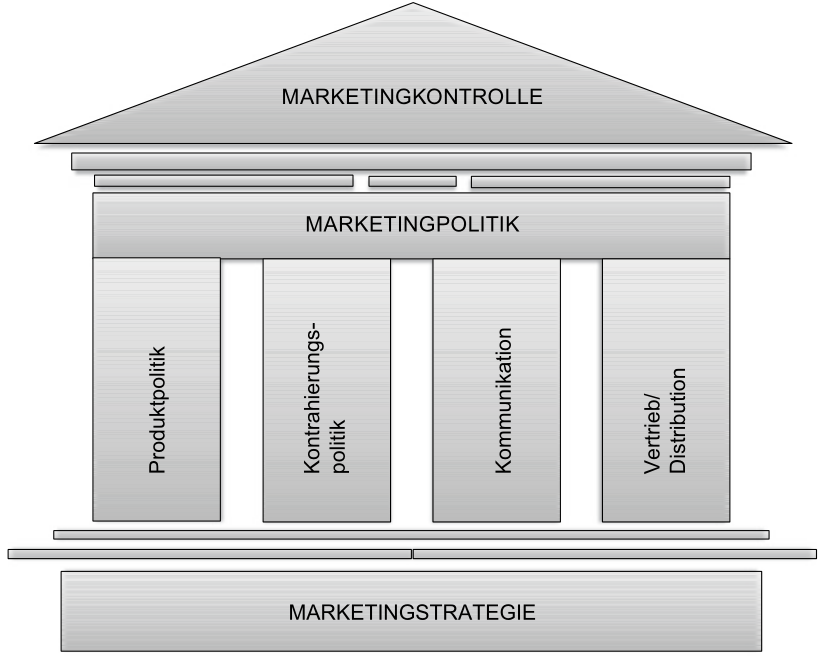
\includegraphics[width=0.7\linewidth]{./images/Marketingcontrolling/Marketingcontrolling} \end{center}

\end{frame}

\begin{frame}{Übung 2: Aufgaben}
\protect\hypertarget{ubung-2-aufgaben}{}

Welche zwei wesentlichen Aufgaben übernimmt das Marketing Controlling?

\begin{enumerate}
[A.]
\tightlist
\item
  Informationsfunktion
\item
  Steuerungsfunktion
\item
  Kontrollfunktion
\item
  Berichterstalltungsfunktion
\end{enumerate}

\note{\textbf{\emph{A und C}}}

\end{frame}

\begin{frame}{Gründe für das Marketing Controlling}
\protect\hypertarget{grunde-fur-das-marketing-controlling}{}

In Marketingpraxis und -wissenschaft nimmt das Thema
Marketingcontrolling eine zentrale Rolle ein.

Während in der Vergangenheit vor allem die bestmögliche Gestaltung der
verschiedenen Instrumente, also der \textbf{Inputfaktoren} des
Marketing, im Fokus stand, ist nun eine Verschiebung hin zum
\textbf{Output} festzustellen.

Hierfür gibt es verschiedene Gründe.

\end{frame}

\begin{frame}{Effizienz und Effektivität}
\protect\hypertarget{effizienz-und-effektivitat}{}

Nachweis von Effizienz und Effektivität des Marketing im Rahmen einer
wertorientierten Unternehmensführung

\begin{itemize}
\tightlist
\item
  Messung des Marketingoutputs
\item
  Transparenz der Ursache-Wirkungsbeziehungen zwischen Marketinginput
  und -output
\end{itemize}

\end{frame}

\begin{frame}{Neue Konzepte}
\protect\hypertarget{neue-konzepte}{}

\begin{itemize}
\tightlist
\item
  Target Costing
\item
  Total Quality Management
\item
  Benchmarking
\item
  Prozessorientierung und Prozesskostenrechnung
\item
  Wissensmanagement, Messung und Steuerung des „Intellectual Capital``
\item
  Performance Measurement, insbesondere Balanced Scorecards
\end{itemize}

\end{frame}

\begin{frame}{Informationssysteme und Technologie}
\protect\hypertarget{informationssysteme-und-technologie}{}

\begin{itemize}
\tightlist
\item
  steigende Integration der Informationssysteme
\item
  höhere Leistungsfähigkeit der Informationsauswertung und -aufbereitung
\item
  verbesserte Informationsverfügbarkeit
\item
  erhöhte Unsicherheit durch Möglichkeiten des E-Business
\end{itemize}

\end{frame}

\begin{frame}{Koordinations- und Umsetzungsdefizite des Marketing}
\protect\hypertarget{koordinations--und-umsetzungsdefizite-des-marketing}{}

\begin{itemize}
\tightlist
\item
  fehlende vertikale Durchgängigkeit ungenügende
\item
  horizontale Integration des operativen Marketing
\item
  Informationsüberflutung des Managements
\end{itemize}

\end{frame}

\begin{frame}{Einsatz von Marketingcontrollingverfahren in der Praxis}
\protect\hypertarget{einsatz-von-marketingcontrollingverfahren-in-der-praxis}{}

\begin{center}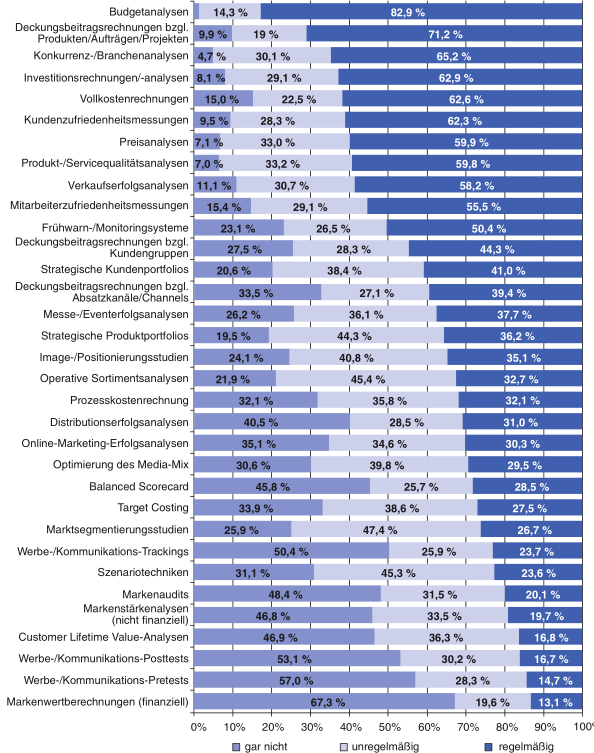
\includegraphics[width=0.48\linewidth]{./images/Marketingcontrolling/Einsatz} \end{center}

\end{frame}

\hypertarget{wirtschaftlichkeitsanalysen}{%
\section{Wirtschaftlichkeitsanalysen}\label{wirtschaftlichkeitsanalysen}}

\begin{frame}{Lernziele}
\protect\hypertarget{lernziele-1}{}

Folgende Wirtschaftlichkeitsanalyseinstrumente als Basisinstrumente
anwenden können:

\begin{itemize}
\tightlist
\item
  Pay-off-Rechnung
\item
  Deckungsbeitragsrechnung
\item
  Break-Even-Analyse
\item
  Kapitalwertmethode
\end{itemize}

\end{frame}

\begin{frame}{Pay-off-Rechnung}
\protect\hypertarget{pay-off-rechnung}{}

Methode zur Ermittlung des Zeitpunkts an dem sich eine Investition
amortisiert. Aussagen über die Rentabilität des Objekts sind damit
jedoch nicht möglich.

\end{frame}

\begin{frame}[fragile]{Vorgehensweise}
\protect\hypertarget{vorgehensweise}{}

Bestimmung des Pay-off-Zeitpunkts mit folgender Formel:

t = \(\frac{Investition}{Einnahmeüberschuss}\) =
\(\frac{ EI }{(p-k_{ v })\times x-(K_{ F }-A)}\)

mit:

\begin{verbatim}
EI: einmalige Investitionsauszahlung zu Beginn 
p:  Verkaufspreis 
kv: variable Stückkosten 
KF: jährliche Fixkosten 
x:  jährliche Absatzmenge 
A:  jährliche Abschreibung 
\end{verbatim}

\end{frame}

\begin{frame}{Übung 3: Pay-off Rechnung}
\protect\hypertarget{ubung-3-pay-off-rechnung}{}

Ende welchen Monats, in welchem Jahr, hat sich die folgende Investition
amortisiert?

geg: EI: 250.000; p: 51; kv: 30; KF: 30.000; x: 5.000; A: 25.000;

\begin{enumerate}
[A.]
\tightlist
\item
  Ende Mai des 2. Jahres
\item
  Ende Mai des 3. Jahres
\item
  Ende Juni des 2. Jahres
\item
  Ende Juli des 3. Jahres
\end{enumerate}

\note{\textbf{\emph{C}}}

\end{frame}

\begin{frame}{Deckungsbeitragsrechnung}
\protect\hypertarget{deckungsbeitragsrechnung}{}

\begin{itemize}
\tightlist
\item
  Methode zur Beurteilung der kurzfristigen Erfolgsträchtigkeit von
  absatzpolitischen Entscheidungen, wie z.\thinspace{}B. der Annahme
  eines Zusatzauftrags bei nicht voll ausgelasteten Kapazitäten.
\item
  Die Deckungsbeitragsrechnung wird als Teilkostenrechnung durchgeführt.
  Langfristig müssen alle Kosten gedeckt sein.
\item
  Vorgehensweise: Der Deckungsbeitrag ergibt sich als Differenz zwischen
  den Erlösen und den variablen Kosten. (Deckungsbeitrag = Betrag der
  zur Deckung der fixen Kosten zur Verfügung steht.)
\end{itemize}

\end{frame}

\begin{frame}[fragile]{Beispiel Deckungsbeitragsrechnung}
\protect\hypertarget{beispiel-deckungsbeitragsrechnung}{}

Ein Produktionswerk ist zu 90 Prozent ausgelastet. Bisher nur Produktion
von Produkt A

Daten: KF: 1.000.000

\begin{verbatim}
Produkt A:  
  kv:   200  
  p:    350  
  
Produkt B:  
  kv:   400  
  p:    490  
  
\end{verbatim}

Kapazität des Werks: 10.000

Wäre es lohnend, die freie Kapazität von 1.000 Stk. Zu nutzen und
Produkt B zu produzieren, wenn nicht mehr von Produkt A abgesetzt werden
könnte?

\end{frame}

\begin{frame}[fragile]{Lösung bei Vollkostenrechnung}
\protect\hypertarget{losung-bei-vollkostenrechnung}{}

Bei Vollkostenrechnung:

\begin{verbatim}
kv: 400  
KF: 1.000.000 / 10.000 =    100 (jährliche Fixkosten pro Stück)  
-------------------------------------------------------------  
Gesamtkosten pro Stück      500  
p: 490  
\end{verbatim}

\end{frame}

\begin{frame}[fragile]{Lösung bei Deckungsbeitragsrechnung}
\protect\hypertarget{losung-bei-deckungsbeitragsrechnung}{}

Bei Deckungsbeitragsrechnung:

\begin{verbatim}
kv: 400  
p:  490  
-------  
db:  90  
\end{verbatim}

db: Stückdeckungsbeitrag

\end{frame}

\begin{frame}{Offene Übung 4: Deckungsbeitragsrechnung}
\protect\hypertarget{offene-ubung-4-deckungsbeitragsrechnung}{}

Ein Mehrprodukt-Unternehmen mit einer jährlichen Produktionskapazität
von 10.000 Einheiten für das Produkt Z steht vor dem Problem, dass von
diesem im laufenden Jahr nur 8.000 Einheiten verkauft werden können. Es
liegen folgende Daten vor:

p:60, kv: 40, KF: 200.000

Ein Freund des Firmeninhabers führt ein Großhandelsunternehmen. Dieser
macht ihm folgendes Angebot: Für Euro 55 pro Stück würde ich auch noch
2000 Einheiten Deines Produkts Z abnehmen. Soll der Firmeninhaber dieses
Angebot annehmen? Führen Sie sowohl eine Vollkosten- als auch eine
Deckungsbeitragsrechnung durch.

\note{db = 55-40 = 15

Stückdeckungsbeitrag x Menge (Zusatzauftrag): 15 x 2.000 = 30.000

Der Zusatzauftrag ermöglicht es, 30.000 der Fixkosten des Produktes Z zu
decken}

\end{frame}

\begin{frame}{Break-Even-Analyse}
\protect\hypertarget{break-even-analyse}{}

Methode zur Berechnung der Gewinnschwelle für neue Produkte (oder auch
andere Investitionen).

Das Verfahren beruht auf folgenden, häufig kritisierten Annahmen:

\begin{itemize}
\tightlist
\item
  Der Preis und die var. Stückkosten sollen über die gesamte
  Analysedauer konstant bleiben (ist fragwürdig).
\item
  Es wird die Kenntnis des Kurvenverlaufs für allen benötigten Parameter
  unterstellt.
\item
  Zinseffekte (zeitlicher Anfall der Geldströme) werden nicht
  berücksichtigt.
\item
  Es wird eine eindeutige Trennbarkeit der Gesamtkosten in fixe und
  variable Bestandteile vorausgesetzt.
\item
  Umsatz- und Gewinninterdependenzen mit anderen Produkten werden nicht
  berücksichtigt.
\end{itemize}

\end{frame}

\begin{frame}{Vorgehensweise Break-Even-Analyse}
\protect\hypertarget{vorgehensweise-break-even-analyse}{}

Es wird die Ausbringungsmenge (bzw. der Zeitpunkt) ermittelt, bei dem
die Erlöse erstmals die Gesamtkosten (var. Kosten + Fixkosten)
übersteigen.

Mit anderen Worten, die Ausbringungsmenge bei der erstmals ein Gewinn
erwirtschaftet wird.

\begin{enumerate}
\tightlist
\item
  Bestimmung der var. Kosten und der Fixkosten sowie des
  Verkaufspreises.
\item
  Berechnung der Break-Even-Menge (Gewinnschwelle) nach folgender
\end{enumerate}

Formel:

M = \(\frac{ K_{ F } }{ p-k_{ v } }\)

\end{frame}

\begin{frame}{Grafische Verdeutlichung Break-Even-Analyse}
\protect\hypertarget{grafische-verdeutlichung-break-even-analyse}{}

\begin{center}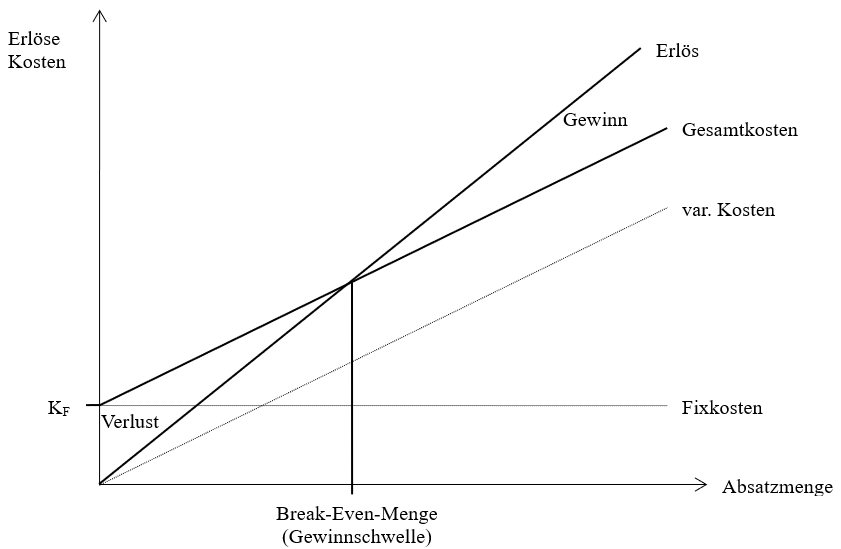
\includegraphics[width=0.7\linewidth]{./images/Marketingcontrolling/Breakeven} \end{center}

\end{frame}

\begin{frame}{Nutzen der Break-Even-Analyse}
\protect\hypertarget{nutzen-der-break-even-analyse}{}

Mit der Break-Even-Analyse lassen sich folgende Fragen beantworten:

\begin{itemize}
\tightlist
\item
  Wie wirkt sich ein Umsatzrückgang bzw. eine Umsatzzunahme auf den
  Gewinn aus?
\item
  Wie wirkt sich eine Kostensenkung bzw. eine Kostensteigerung auf den
  Gewinn aus?
\item
  können zusätzliche Marketing-Kosten den Umsatz steigern?
\item
  Kann eine Preiserhöhung (-senkung) aufgrund der Nachfragestruktur den
  Gewinn steigern?
\item
  Um wieviel muss der Umsatz steigen, um zusätzliche Kosten zu decken?
\item
  Wie groß ist der Deckungsbeitrag bei unterschiedlichen Absatzmengen?
\end{itemize}

\end{frame}

\begin{frame}{Beispiel Break-Even-Analyse}
\protect\hypertarget{beispiel-break-even-analyse}{}

geg:

KF: 20.000 pro Jahr\\
p: 150\\
kv: 100

Gewinnschwelle = M = \(\frac{ 20.000 }{ 150-100 }\) =
\(\frac{ 20.000 }{ 50 }\) = 400

Folgende Schätzungen liegen für den jährlichen Absatz vor:

\begin{itemize}
\tightlist
\item
  optimistisch: 500
\item
  pessimistisch: 350
\item
  relative sicher: 425
\end{itemize}

Bei 400 verkauften Stück sind die Fixkosten gedeckt.

\begin{itemize}
\tightlist
\item
  Relativ sicherer Gewinn = 25 x 50 = 1250
\item
  optimistischer Fall: Gewinn = 100 x 50 = 5000
\item
  pessimistischer Fall: Verlust = Unterdeckung = 50 x 50 = 2500
\end{itemize}

\end{frame}

\begin{frame}{Grafik zum Beispiel}
\protect\hypertarget{grafik-zum-beispiel}{}

\begin{center}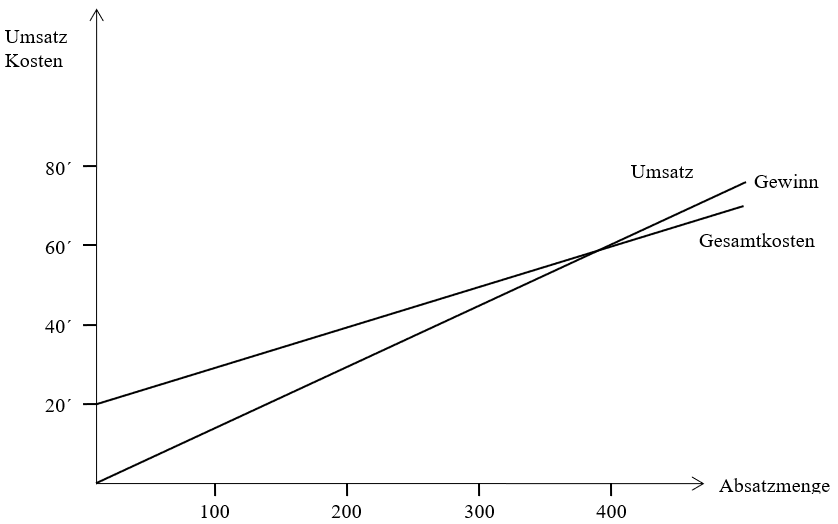
\includegraphics[width=0.7\linewidth]{./images/Marketingcontrolling/Breakeven2} \end{center}

\end{frame}

\begin{frame}{Offene Übung 5: Break-Even A}
\protect\hypertarget{offene-ubung-5-break-even-a}{}

Die Firma SUNSTAR stellt elektrische Gartengeräte her. Der
Entwicklungsabteilung des Unternehmens ist es gelungen einen marktreifen
Solarmäher zu konstruieren. Die Geschäftsleitung beauftragt Sie als
neuen Mitarbeiter der Marketingabteilung zu ermitteln, bei welcher
jährlichen Absatzmenge das neue Produkt die Gewinnzone erreicht. Sie
stellt ihnen folgende Daten zur Verfügung:

Name des Mähers: SolarCut 2000\\
Verkaufspreis: Euro 900\\
var. Kosten pro Stück: Euro 600\\
jährliche Fixkosten (für Abschreibungen, Werbung, etc.): Euro 2.400.000

Ermitteln Sie rechnerisch und graphisch den Break-Even-Point.

\note{Schwellenmenge = M = \(\frac{ 2.400.000 }{ 900 - 600 }\) = 8.000

\begin{center}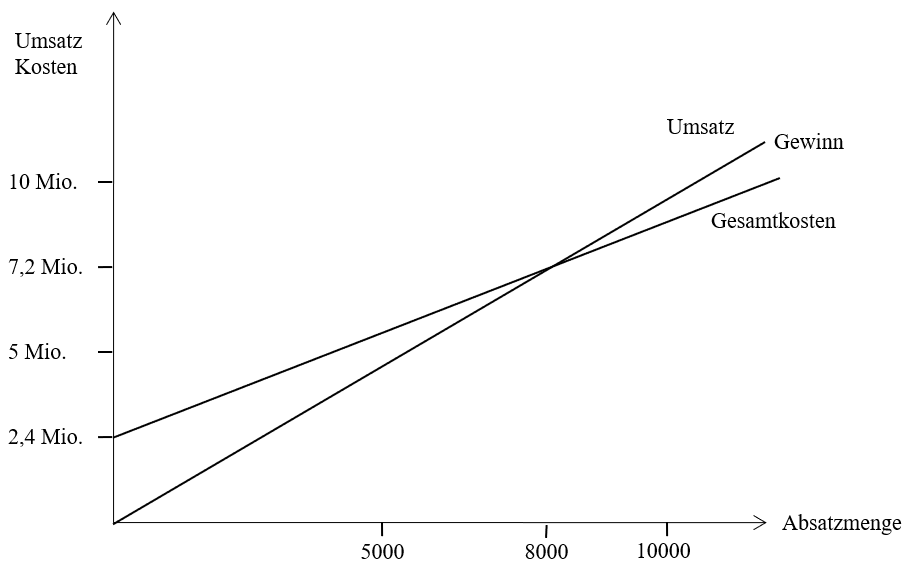
\includegraphics[width=0.7\linewidth]{./images/Marketingcontrolling/Breakeven3} \end{center}}

\end{frame}

\begin{frame}{Offene Übung 6: Break-Even B}
\protect\hypertarget{offene-ubung-6-break-even-b}{}

Da die Firma die Firma SUNSTAR als erster Anbieter der Branche einen
Solarmäher auf dem Markt anbieten kann, ist die Geschäftsleitung bzgl.
der Absatzchancen optimistisch und rechnet mit einem Absatz von 11.000
Stück pro Jahr. Gleichzeitig überlegt sie, die Werbekosten pro Jahr um
Euro 400.000 zu erhöhen. Da sich das Produkt in diesem Fall als
``echtes'' Markenprodukt in den Köpfen der Verbraucher festsetzen
sollte, geht man davon aus, dass auch bei einem Verkaufspreis von Euro
1000 noch 11.000 Mäher verkauft werden können.

Wie hoch wäre die Gewinnschwelle in diesem Fall? Welche Veränderungen
ergeben sich in der graphischen Lösung?

\note{Schwellenmenge = M =
\(\frac{ 2.400.000 + 400.000 }{ 1.000 - 600 }\) = 7.000

\begin{center}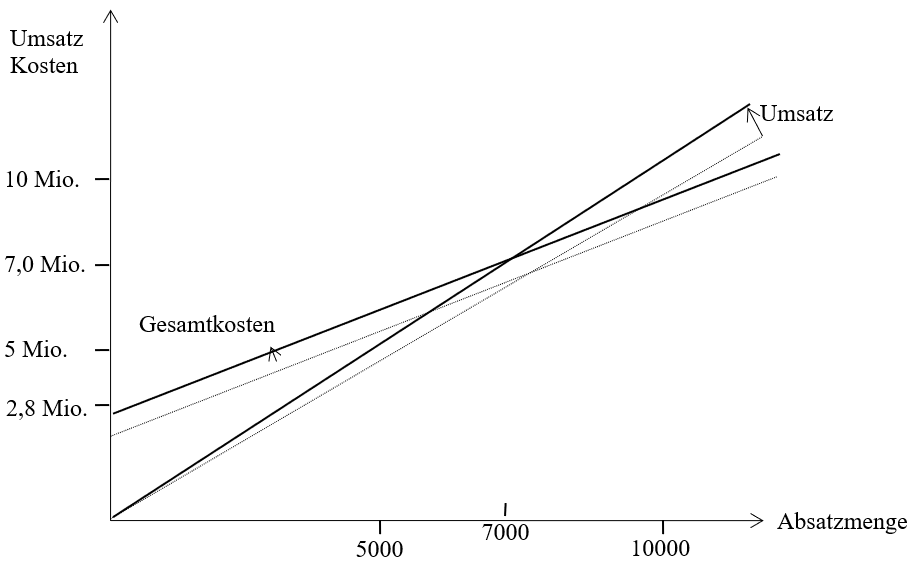
\includegraphics[width=0.7\linewidth]{./images/Marketingcontrolling/Breakeven4} \end{center}}

\end{frame}

\begin{frame}{Übung 7: Break-Even 2}
\protect\hypertarget{ubung-7-break-even-2}{}

Für welche der beiden Alternativen sollte sich das Unternehmen aufgrund
der vorliegenden Daten entscheiden?

\begin{enumerate}
[A.]
\tightlist
\item
  A
\item
  B
\end{enumerate}

\note{Gewinn (A) = (900 - 600) x 11.000 - 2.400.000 = 900.000

Gewinn (B) = (1.000 - 600) x 11.000 - 2.800.000 = 1.600.000

oder: 400 x 4.000 = 1.600.000

Entscheidung für Alt. 2.}

\end{frame}

\begin{frame}{Kapitalwertmethode}
\protect\hypertarget{kapitalwertmethode}{}

\begin{itemize}
\tightlist
\item
  Methode zur Beurteilung der Vorteilhaftigkeit einer Investition im
  Vergleich zu einer Geldanlage oder auch zu alternativen Investitionen.
\item
  Das Verfahren ist dynamisch und berücksichtigt Zinsen
  (Kalkulationszinssatz).
\end{itemize}

Vorgehensweise:

Unter der Zuhilfenahme von Umrechnungstabellen werden zukünftige
Einzahlungsüberschüsse auf den ``Startzeitpunkt'' der Investition
abgezinst. Die Summe dieser Beträge wird zu der Investitionsauszahlung
in Beziehung gesetzt.

\end{frame}

\begin{frame}{Kapitalwertmethode Beispiel(1)}
\protect\hypertarget{kapitalwertmethode-beispiel1}{}

Wieviel sind Euro 1.000 in einem Jahr, wenn ich sie zu 10 \% anlege?

1.000 x (1+i) = 1.000 x 1,1 = 1.100

i: Zinssatz

\end{frame}

\begin{frame}{Kapitalwertmethode Beispiel(2)}
\protect\hypertarget{kapitalwertmethode-beispiel2}{}

Wieviel sind Euro 15.000, die ich in einem Jahr erhalte, heute Wert,
wenn der Zinssatz auf dem Kapitalmarkt 10 \% beträgt?

\(\frac{ 15.000 }{ 1+i }\) = \(\frac{ 15.000 }{ 1,1 }\) = 15.000 *
\(\frac{ 1 }{ 1,1 }\) = 13.635

\end{frame}

\begin{frame}{Kapitalwertmethode Beispiel(3)}
\protect\hypertarget{kapitalwertmethode-beispiel3}{}

Wieviel sind Euro 15.000, die ich in zwei Jahren erhalte heute Wert,
wenn der Zinssatz auf dem Kapitalmarkt 10 \% beträgt?

\(\frac{ 15.000 }{(1+i)^{2} }\) = \(\frac{ 15.000 }{1,1^{2} }\) = 15.000
* \(\frac{ 1 }{1,1^{2} }\) = 12.390

Umrechnungsfaktor bei 3 Jahren: \(\frac{ 1 }{(1,1)^{3} }\)

\end{frame}

\begin{frame}{Übung 8: Kapitalwertmethode}
\protect\hypertarget{ubung-8-kapitalwertmethode}{}

Sie haben die Möglichkeit einen Betrag von Euro 20.000 bei einem
Zinssatz von 5 Prozent für 5 Jahre anzulegen oder diesen Betrag in ein
Projekt zu investieren. Für das Projekt werden folgende Ein- und
Auszahlungen in den nächsten 5 prognostiziert:

Zu Beginn des Projekts (t = 0): Investitionsauszahlung: -20.000

Jahre 1 bis 5 (t = 1, \ldots{}, 5):

Einzahlungen pro Jahr = 10.000\\
Auszahlungen pro Jahr = 5.000

Welche Alternative sollten Sie nach der Kapitalwertmethode wählen?

\begin{enumerate}
[A.]
\tightlist
\item
  Geldanlage
\item
  Projekt
\end{enumerate}

\note{Kapitalwerte des Projekt = 21.650 - 20.000

also \textgreater{} 0 und deshalb der Geldanlage vorzuziehen.}

\end{frame}

\hypertarget{operatives-marketing-controlling}{%
\section{Operatives Marketing
Controlling}\label{operatives-marketing-controlling}}

\begin{frame}{Lernziele}
\protect\hypertarget{lernziele-2}{}

\begin{itemize}
\tightlist
\item
  Funktion des operativen Marketing Controllings verstehen.
\item
  Zusammenhang zwischen Planung und Controlle verstehen.
\item
  Abweichungsanalyse anwenden können.
\item
  Das Konzept der Kundenzufriedenheit verstehen und evaluieren.
\item
  Kundenzufriedenheitsmessung durchführen können.
\item
  ABC-Analysen einordnen können.
\item
  Customer-Lifetime value verstehen und einordnen können
\end{itemize}

\end{frame}

\begin{frame}{Idee des operativen Marketing-Controllings}
\protect\hypertarget{idee-des-operativen-marketing-controllings}{}

\begin{itemize}
\tightlist
\item
  Da die strategische Marketingplanung den Orientierungsrahmen bildet,
  steht die operative Marketingplanung in einer instrumentellen
  Vollzugsfunktion.
\item
  Hierbei listet man zunächst alle Mittel und Massnahme auf, die zur
  Zielerreichung beitragen.
\item
  Daraufhin steht die Auswahl, Gewichtung und Ausgestaltung der
  marketingpolitischen Aktivitäten und deren Verzahnung zu einem
  zielführenden Mix im Blickpunkt.
\item
  Den Gegenstand des operativen Marketing-Controllings bildet eine
  Überprüfung, ob und inwieweit sich die realisierten Maßnahmen als
  richtig und effizient erweisen.
\end{itemize}

\end{frame}

\begin{frame}{Marketing-Kontrolle als Feedbackfunktion}
\protect\hypertarget{marketing-kontrolle-als-feedbackfunktion}{}

\begin{itemize}
\tightlist
\item
  Die Kontrolle erschöpft sich jedoch nicht darin, Differenzen zwischen
  geplanter und tatsächlich eingetretener Wirkung festzustellen, sondern
  umschließt darüber hinaus auch die Analyse der Abweichungsursachen.
\item
  Die gewonnenen Erkenntnisse geben dem Unternehmen Hinweise für eine
  Modifikation der Marketingplanung.
\item
  Die operative Marketingkontrolle übernimmt damit eine
  Feedback-Funktion, indem sie Anstöße für einen neuen Planungsprozess
  liefert.
\end{itemize}

\end{frame}

\begin{frame}{Vorgehensweise bei der Planung und Kontrolle}
\protect\hypertarget{vorgehensweise-bei-der-planung-und-kontrolle}{}

\begin{center}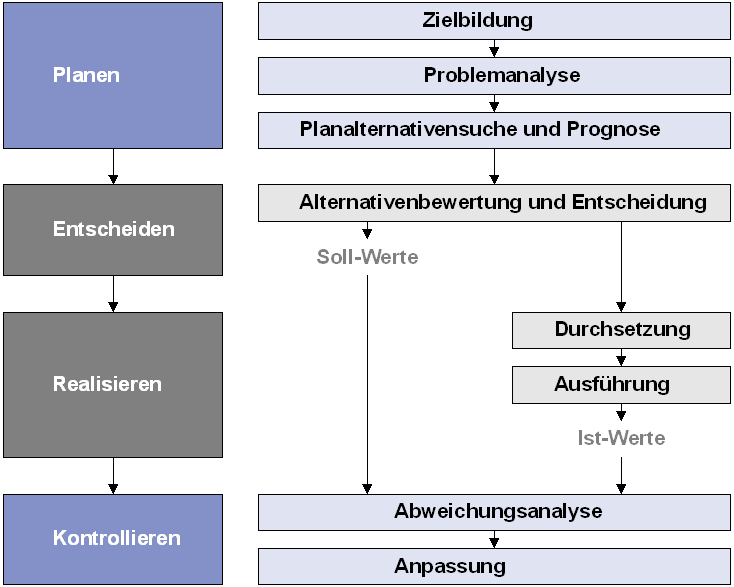
\includegraphics[width=0.7\linewidth]{./images/Marketingcontrolling/Vorgehensweise1} \end{center}

\end{frame}

\begin{frame}{Die Soll-Ist Abweichungsanalyse}
\protect\hypertarget{die-soll-ist-abweichungsanalyse}{}

\begin{center}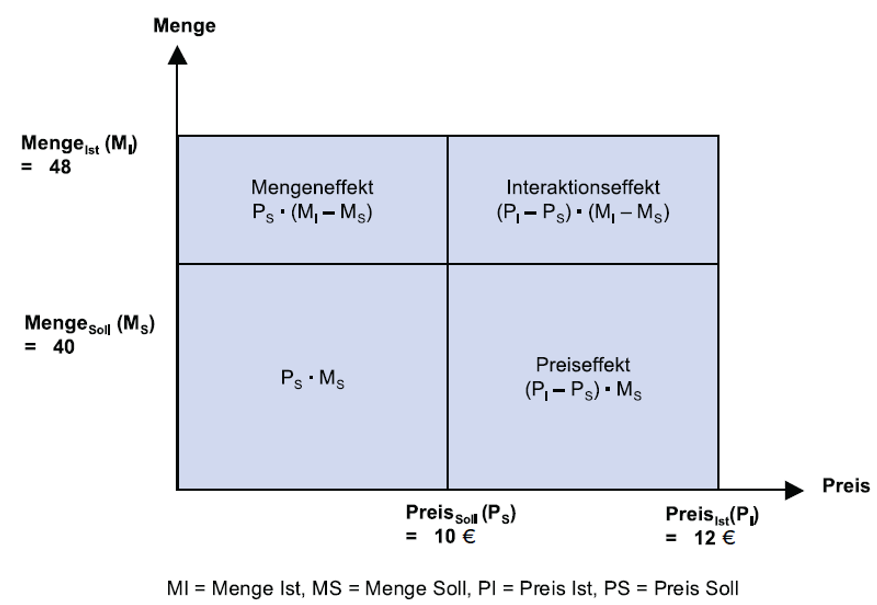
\includegraphics[width=0.7\linewidth]{./images/Marketingcontrolling/Abweichungsanalyse} \end{center}

\end{frame}

\begin{frame}{Grundidee der Abweichungsanalyse}
\protect\hypertarget{grundidee-der-abweichungsanalyse}{}

\begin{itemize}
\tightlist
\item
  Wie aus der voranstehenden Abbildung ersichtlich, sollte bei einem
  Preis von 10 eine Menge von 40 abgesetzt werden.
\item
  Tatsächlich konnten 48 Einheiten bei einem Preis von 12 abgesetzt
  werden.
\item
  Insofern wurde der geplante Umsatz von €400 um €176 überschritten.
\item
  Diese Umsatzabweichung von €176 lässt sich in verschiedene Effekte
  unterteilen.
\item
  Der am Markt durchsetzbare höhere Preis von €12 statt €10 führt zu
  einem Umsatzplus von €80 (Preiseffekt).
\item
  Zudem konnten 8 Einheiten mehr abgesetzt werden als geplant, was eben
  €80 zusätzlichen Umsatz generiert (Mengeneffekt).
\item
  Durch das gleichzeitige Wirksamwerden von Preis- und Mengeneffekt
  entsteht ein Interaktionseffekt, der zusätzlich €16 Umsatzsteigerung
  bringt.
\end{itemize}

\end{frame}

\begin{frame}[shrink]{Berechnung des Preis-, Mengen- und
Interaktionseffekts}
\protect\hypertarget{berechnung-des-preis--mengen--und-interaktionseffekts}{}

\begin{center}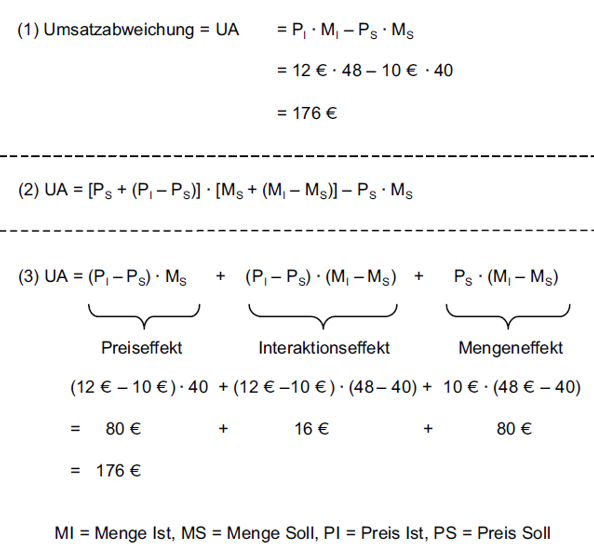
\includegraphics[width=0.7\linewidth]{./images/Marketingcontrolling/Preismengeneffekt} \end{center}

\end{frame}

\begin{frame}{Interpretation des Preis-, Mengen- und
Interaktionseffekts}
\protect\hypertarget{interpretation-des-preis--mengen--und-interaktionseffekts}{}

Der Preiseffekt entsteht aus einem durchgesetzten Preis, der über dem
Planpreis liegt. Der Mengeneffekt resultiert aus einer abgesetzten
Menge, die die Planmenge übertrifft. Der Interaktionseffekt ergibt sich
aus dem gleichzeitigen Wirksamwerden des Preis- und Mengeneffekts. Die
Zerlegung der Abweichung in diese drei Effekte erlaubt einen Rückschluss
auf die Wirksamkeit der verschiedenen absatzwirtschaftlichen
Instrumente.

\end{frame}

\begin{frame}{Abweichungsanalyse}
\protect\hypertarget{abweichungsanalyse}{}

\begin{itemize}
\tightlist
\item
  Für das Abweichungsgespräch zwischen dem Controller und dem
  Marketingmanager erweist es sich als hilfreich, nicht nur die
  einzelnen Effekte voneinander zu unterscheiden, sondern auch endogene
  und exogene Einflüsse zu trennen.
\item
  Hierbei umfassen die exogenen Einflüsse alle Einflussfaktoren, die auf
  den Markt wirken und nicht unmittelbar vom Unternehmen beeinflusst
  werden können.
\item
  Dagegen betreffen die endogenen Effekte das Unternehmen; zu ihnen
  zählen alle Einflüsse, die auf Kunden- und Konkurrenzreaktionen
  beruhen.
\end{itemize}

\end{frame}

\begin{frame}{Determinanten auf Preis- und Absatzmenge}
\protect\hypertarget{determinanten-auf-preis--und-absatzmenge}{}

\begin{center}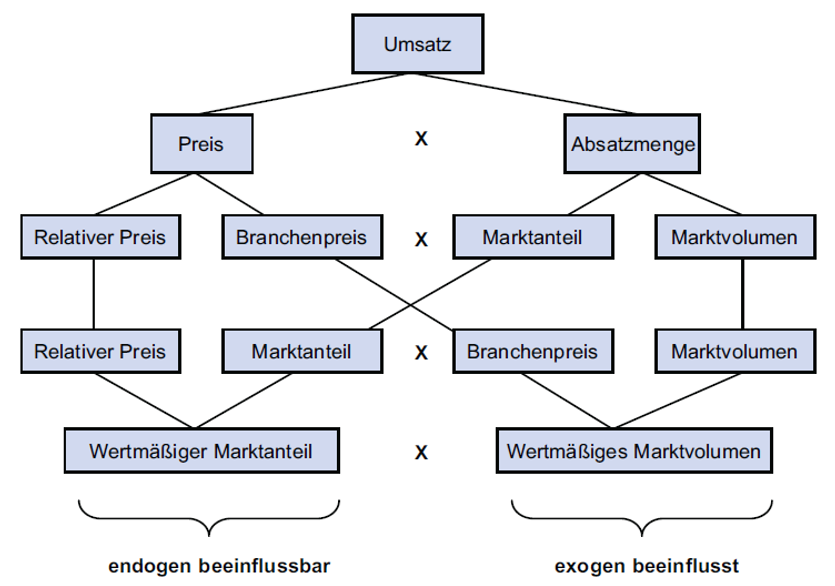
\includegraphics[width=0.7\linewidth]{./images/Marketingcontrolling/Abweichungsanalyse2} \end{center}

\end{frame}

\begin{frame}{Grundstruktur der Determinantenidentifikation}
\protect\hypertarget{grundstruktur-der-determinantenidentifikation}{}

\begin{itemize}
\tightlist
\item
  Zunächst erfolgt eine Aufspaltung des Umsatzes in den Preis und die
  Absatzmenge, die ihrerseits in den relativen Preis und den
  Branchenpreis bzw. den Marktanteil und das Marktvolumen zerfallen.
\item
  Marktvolumen und Branchenpreis sind durch den Marketingmanager nicht
  beeinflussbar.
\item
  Hingegen hängen der relative Preis und der Marktanteil von den
  marketingpolitischen Aktivitäten des Unternehmens ab.
\item
  Diese Analyse erlaubt eine Identifikation jener Größen, die vom
  Unternehmen beeinflussbar sind und solchen, die das Unternehmen nicht
  beeinflussen kann. Auf Basis einer solchen Auswertung lassen sich die
  marketingpolitischen Instrumente ausgestalten.
\end{itemize}

\end{frame}

\begin{frame}{Ansätze zur Messung der Kundenzufriedenheit}
\protect\hypertarget{ansatze-zur-messung-der-kundenzufriedenheit}{}

\begin{center}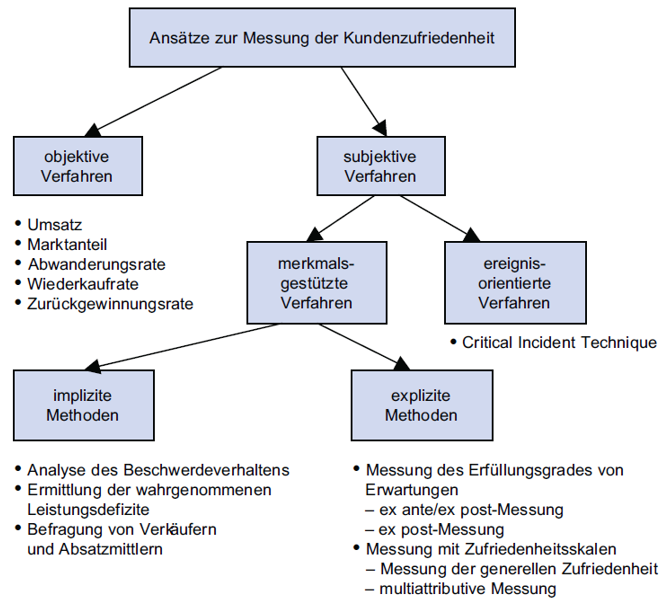
\includegraphics[width=0.7\linewidth]{./images/Marketingcontrolling/Zufriedenheit} \end{center}

\end{frame}

\begin{frame}{Die Techniken zur Erfassung der Kundenzufriedenheit im
Überblick}
\protect\hypertarget{die-techniken-zur-erfassung-der-kundenzufriedenheit-im-uberblick}{}

\begin{itemize}
\tightlist
\item
  In der Unternehmenspraxis finden objektive Verfahren die größte
  Beachtung. Diese Methoden erfassen Größen, die nicht auf der
  Einschätzung von Betroffenen basieren. Hierzu zählen insbesondere
  Umsatz- und Marktanteilszahlen sowie die Loyalitätsrate.
\item
  Da die individuelle Wahrnehmung des Verhaltens treibt, fordern viele
  Wissenschaftler und Praktiker subjektive Kriterien.
\item
  Diese lassen sich in merkmalsgestützte und ereignisorientierte
  Verfahren unterteilen.
\item
  Während man bei den merkmalsgestützten Verfahren itemweise befragt,
  zeichnet sich das ereignisorientierte Vorgehen durch eine Erfassung
  einer Episode auf.
\item
  In der Praxis bietet sich eine Kombination von merkmalsgestützten und
  ereignisorientierten Verfahren an, da sie unterschiedliche Facetten
  der Zufriedenheit erfassen.
\end{itemize}

\end{frame}

\begin{frame}{Formen der Zufriedenheit}
\protect\hypertarget{formen-der-zufriedenheit}{}

\begin{center}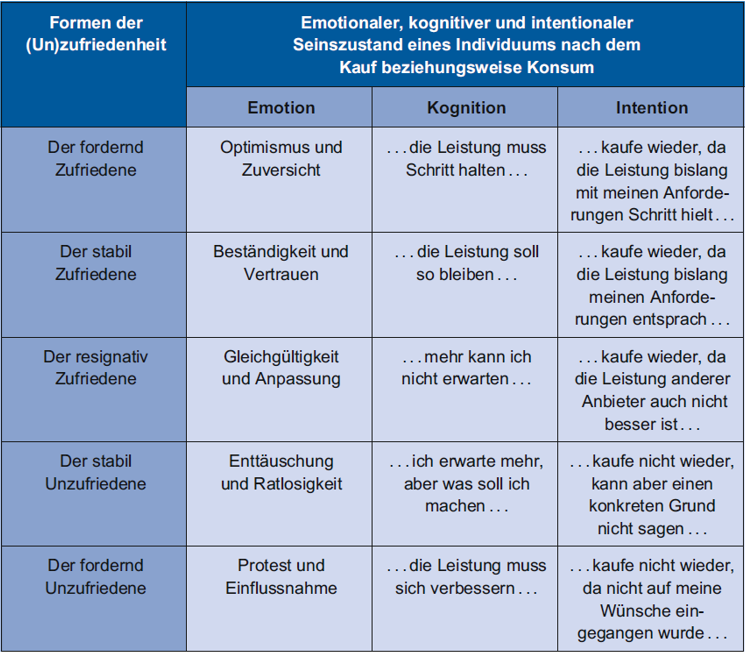
\includegraphics[width=0.7\linewidth]{./images/Marketingcontrolling/Zufriedenheitsformen} \end{center}

\end{frame}

\begin{frame}{Zufriedenheit und Unzufriedenheit und ihre Wirkung auf das
Verhalten}
\protect\hypertarget{zufriedenheit-und-unzufriedenheit-und-ihre-wirkung-auf-das-verhalten}{}

\begin{itemize}
\tightlist
\item
  Zumeist kennt das Unternehmen nur den fordernd Unzufriedenen und den
  fordernd Zufriedenen.
\item
  Der resignative Zufriedene äußert sich nicht mehr, da er keine
  Veränderungsmöglichkeiten sieht. Auch die stabil Zufriedenen wie
  stabil Unzufriedenen geben dem Unternehmen kaum Feedback.
\item
  Insofern sind die Marktinformationen, die das Unternehmen erhält, nur
  auf die Aussagen weniger Individuen zurückzuführen, die in keiner
  Weise die Kundenbasis repräsentieren.
\end{itemize}

\end{frame}

\begin{frame}{Die Kundenbewertung mit verschiednen Ansätzen}
\protect\hypertarget{die-kundenbewertung-mit-verschiednen-ansatzen}{}

\begin{center}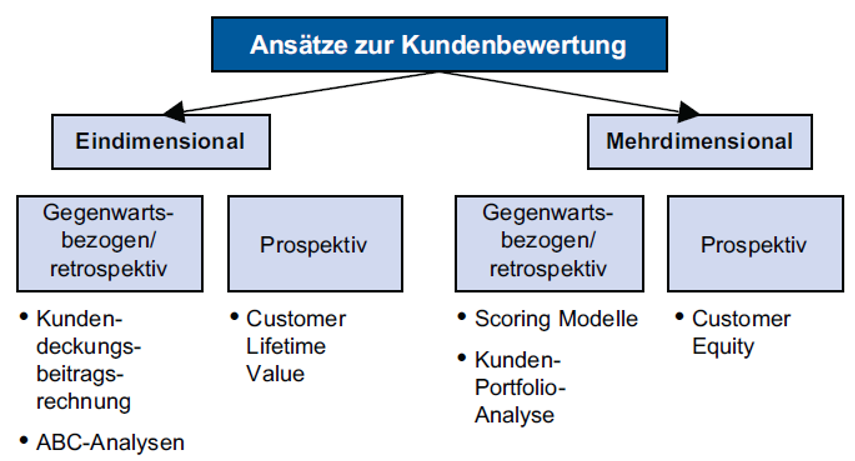
\includegraphics[width=0.7\linewidth]{./images/Marketingcontrolling/Kundenbewertung} \end{center}

\end{frame}

\begin{frame}{Kundenwertmessung als Marketingaufgabe}
\protect\hypertarget{kundenwertmessung-als-marketingaufgabe}{}

\begin{itemize}
\tightlist
\item
  Die Erfassung des Kundenwerts gehört zu den zentralen Aufgaben im
  Marketing.
\item
  Nur wenn die Kunden im Hinblick auf ihren Kundenwert bekannt sind,
  lassen sich die marketingpolitischen Aktivitäten kundenorientiert
  ausgestalten.
\item
  In Abhängigkeit des Werts eines Kunden, sind unterschiedliche
  marketingpolitische Aktivitäten einzusetzen. Durch die
  Kundenwertmessung lässt sich der Einsatz der marketingpolitischen
  Aktivitäten finanzwirtschaftlich rechtfertigen.
\end{itemize}

\end{frame}

\begin{frame}{Grundstruktur einer Kundendeckungsbeitragsrechnung}
\protect\hypertarget{grundstruktur-einer-kundendeckungsbeitragsrechnung}{}

\begin{center}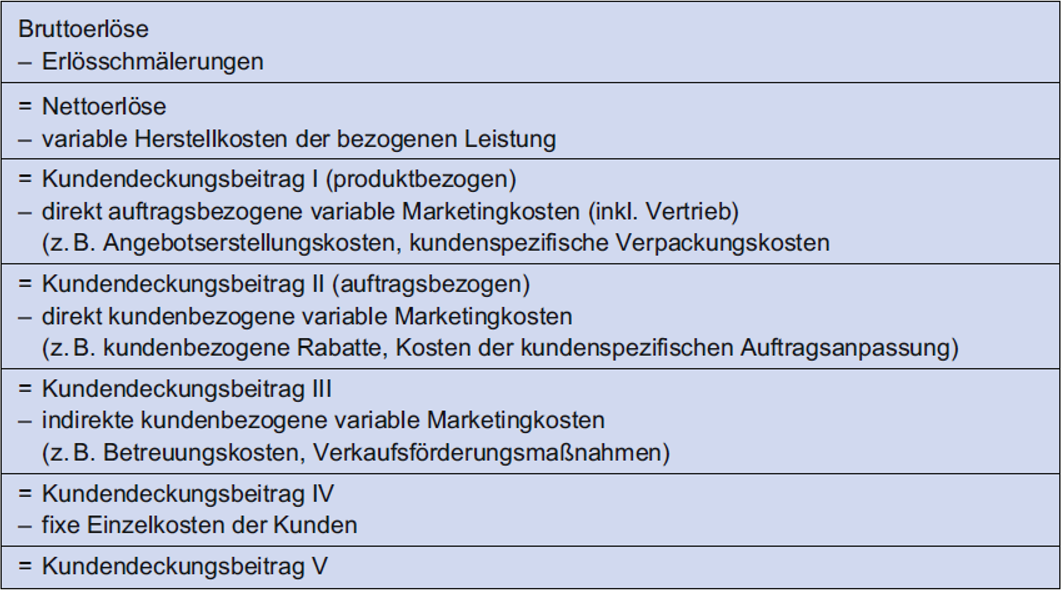
\includegraphics[width=0.7\linewidth]{./images/Marketingcontrolling/Kundendeckungsbeitragsrechnung} \end{center}

\end{frame}

\begin{frame}{Idee der Kundendeckungsbeitragsrechnung}
\protect\hypertarget{idee-der-kundendeckungsbeitragsrechnung}{}

\begin{itemize}
\tightlist
\item
  Die Kundendeckungsbeitragsrechnung dient dazu, eine Facette des
  Kundenwerts zu liefern. Gemeinsam mit Schätzungen über das zukünftige
  Verhalten des Kunden lässt sich die Kundendeckungsbeitragsrechnung zur
  Ermittlung des - Kundenwerts einsetzen.
\item
  Voraussetzung für eine aussagekräftige Kundendeckungsbeitragsrechnung
  ist eine zweckneutrale Grundrechnung.
\item
  Darauf aufbauend können Auswertungen für Kunden als Kalkulationsobjekt
  vorgenommen werden.
\end{itemize}

\end{frame}

\begin{frame}{Grundstruktur der umsatzbezogenen ABC-Analyse}
\protect\hypertarget{grundstruktur-der-umsatzbezogenen-abc-analyse}{}

\begin{center}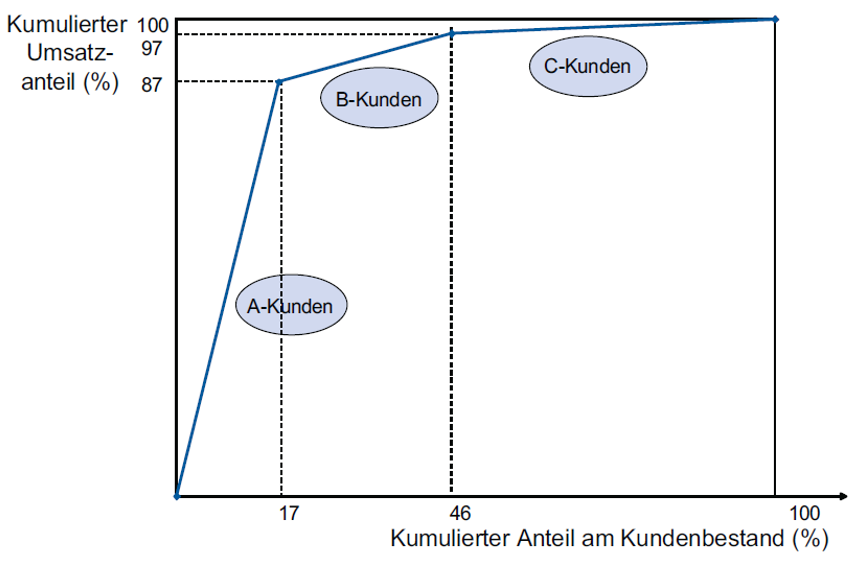
\includegraphics[width=0.48\linewidth]{./images/Marketingcontrolling/ABC} \end{center}

\end{frame}

\begin{frame}{Idee der ABC-Analyse}
\protect\hypertarget{idee-der-abc-analyse}{}

\begin{itemize}
\tightlist
\item
  Bei der ABC-Analyse geht es um eine Klassifikation der Kunden nach
  ihrer Wichtigkeit anhand des Umsatzes bzw. Deckungsbeitrags.
\item
  Kundenumsätze können direkt vom Rechnungswesen entnommen werden, und
  die anschließende geordnete Aggregation der Kunden nach dem Umsatz ist
  schnell und leicht durchgeführt.
\item
  Kritisch anzumerken ist allerdings, dass zwischen dem Gesamtumsatz und
  der Profitabilität einzelner Kundenbeziehungen nicht zwingend eine
  lineare Beziehung bestehen muss.
\item
  Den einzelnen Segmenten (A,B,C) sind unterschiedliche
  marketingpolitische Aktivitäten zuzuordnen.
\end{itemize}

\end{frame}

\begin{frame}{Übung 9: Zufriedenheitsmessung}
\protect\hypertarget{ubung-9-zufriedenheitsmessung}{}

Häufig bedeutet die Erfassung der Kundenzufriedenheit einen beachtlichen
Aufwand für das Unternehmen. Insofern sind Marketingmanager bestrebt,
den Erfassungsaufwand zu reduzieren bzw. die Datenerfassung möglichst
effizient zu gestalten. Stellen Sie sich vor, Sie seien Manager einer
Fluglinie und hätten bereits eine ABC-Analyse ihrer Kundenbasis
durchgeführt. Diese ABC-Analyse soll im Folgenden die Basis bilden, um
unterschiedliche Varianten von Kundenzufriedenheitsanalysen
durchzuführen.

Erläutern Sie die Grundidee der ABC-Analyse.

\note{Bei der ABC-Analyse geht es um die Klassifikation der Kunden nach
ihre Richtigkeit anhand des Umsatzes bzw. Deckungsbeitrags. Gerade
umsatzbezogene ABC-Analysen sind in der Praxis beliebt. Kundenumsätze
können direkt dem Berechnungswesen entnommen werden und die
anschliessende geordnete Aggregation der Kunden nach dem Umsatz ist
leicht und schnell durchgeführt. Kritisch anzumerken ist allerdings,
dass zwischen dem Gesamtumsatz und der Profitabilität einzelner
Kundenbeziehungen nicht zwingend eine lineare Beziehung bestehen muss.
Vor diesem Hintergrund erscheint eine deckungsbeitragsbezogene
ABC-Analyse geeigneter.}

\end{frame}

\begin{frame}{Übung 10: Grundstruktur Zufriedenheitsbefragung}
\protect\hypertarget{ubung-10-grundstruktur-zufriedenheitsbefragung}{}

Diskutieren Sie die Grundstruktur einer Zufriedenheitsbefragung, nach
A-, B- und C-Kunden.

\note{\textbf{Kundenzufriedenheitsanalyse bei A-Kunden:} Bei A-Kunden
geht es darum, ein vollumfängliches Bild über deren Befindlichkeiten zu
erfassen. Hierzu sollten die verschiedenen Instrumente zur
Rekonstruktion der Kundenzufriedenheit zum Einsatz kommen, wie etwa
klassischer Fragebogen, offenes Interview sowie objektive Methoden
(Umsatzentwicklung pro Kunde \mbox{c.\thinspace{}).}\xspace{} Darüber
hinaus könnte ein Kundenbeirat, der aus A-Kunden besteht, in Betracht
kommen, um dem Top-Management direkt Feedback über die
Unternehmensleistung zu geben.

\textbf{Bei den B-Kunden} ist vorstellbar, dass lediglich ein Fragebogen
zum Einsatz kommt, der umfassend ist, und die wesentlichen
Leistungsfacetten beinhaltet.

\textbf{Bei den C-Kunden} könnte man sich vorstellen, dass man lediglich
die kritischen Leistungsdimensionen (vgl. dazu Zufriedenheitsbefragung
bei den A- und B-Kunden) erfasst, um ein Bild über die
Leistungsverbesserung zu erzielen.}

\end{frame}

\begin{frame}{Übung 11: Grenzen Zufriedenheitsbefragung}
\protect\hypertarget{ubung-11-grenzen-zufriedenheitsbefragung}{}

Erläutern Sie die Grenzen der Kundenzufriedenheitsbefragung.

\note{Das Problem der Kundenzufriedenheit besteht darin, dass sich
zumeist nur jene Kunden äussern, die sehr zufrieden oder sehr
unzufrieden sind. Die grosse, graue Menge ist schwer für die Abgabe
eines Zufriedenheitsurteils zu mobilisieren. Insofern ist bei der
Analyse und Interpretation der Kundenzufriedenheitswerte darauf zu
achten, aus welchem Sample die Nennungen stammen. Eine unreflektierte
Übertragung der Analyseergebnisse in Handlungsempfehlungen könnte nicht
adäquat vor dem Hintergrund der realen Gegebenheiten und der verzerrten
Stichprobe sein.}

\end{frame}

\begin{frame}{Definition des Customer Lifetime Value}
\protect\hypertarget{definition-des-customer-lifetime-value}{}

\begin{center}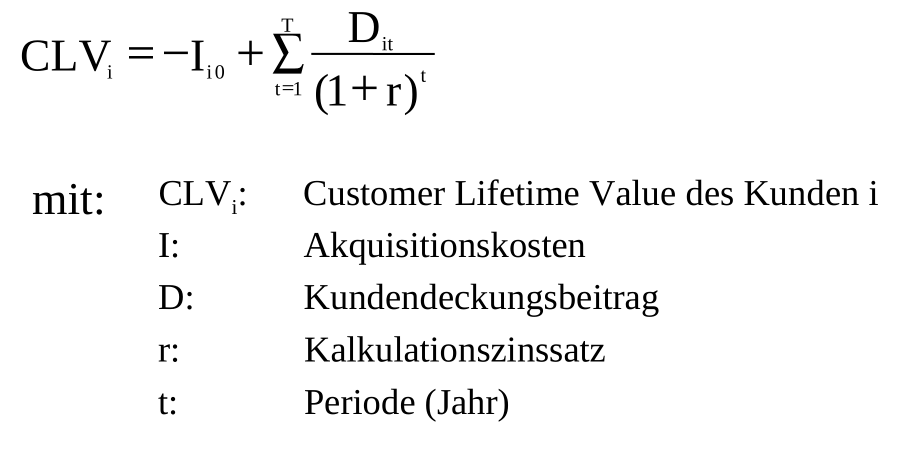
\includegraphics[width=0.8\linewidth]{./images/Marketingcontrolling/CLV} \end{center}

\end{frame}

\begin{frame}{Möglicher Verlauf der Kundenbindungs-, Erlös-, CLV- und
Deckungsbeitragskurve}
\protect\hypertarget{moglicher-verlauf-der-kundenbindungs--erlos--clv--und-deckungsbeitragskurve}{}

\begin{center}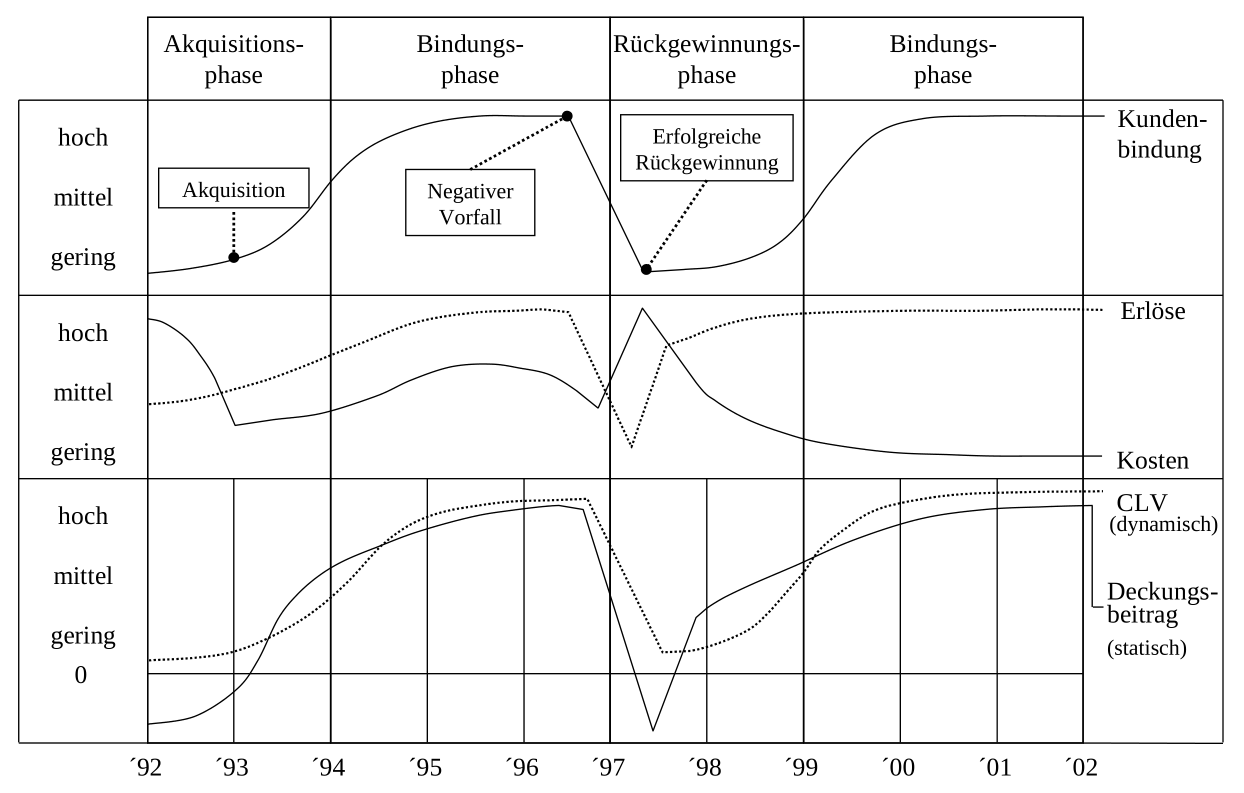
\includegraphics[width=0.8\linewidth]{./images/Marketingcontrolling/CLV2} \end{center}

\end{frame}

\begin{frame}{Zahlenbeispiel zur Berechnung des CLV für einen
Individualkunden}
\protect\hypertarget{zahlenbeispiel-zur-berechnung-des-clv-fur-einen-individualkunden}{}

\begin{center}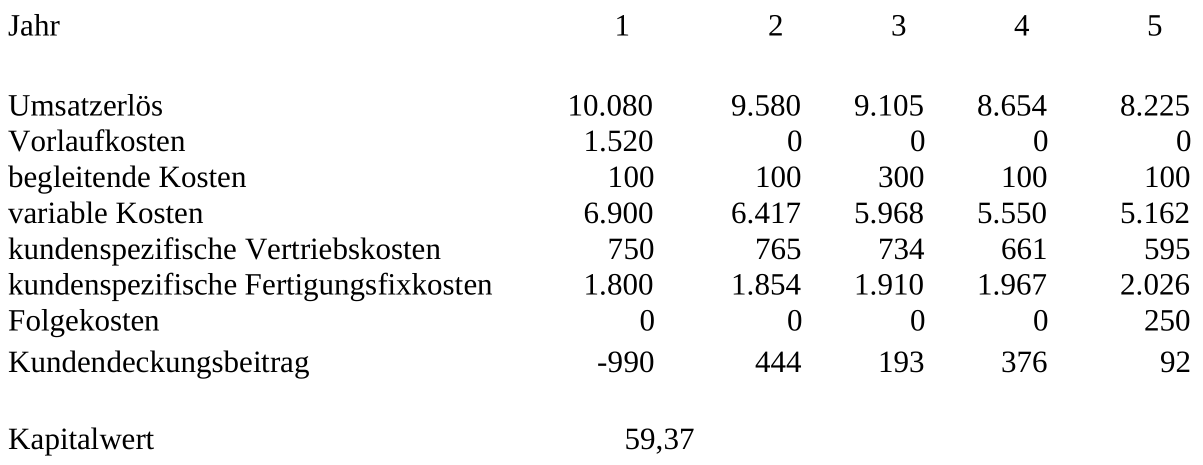
\includegraphics[width=0.8\linewidth]{./images/Marketingcontrolling/CLV3} \end{center}

\end{frame}

\begin{frame}{Zahlenbeispiel zur Berechnung des CLV für einen typischen
Kunden}
\protect\hypertarget{zahlenbeispiel-zur-berechnung-des-clv-fur-einen-typischen-kunden}{}

\begin{center}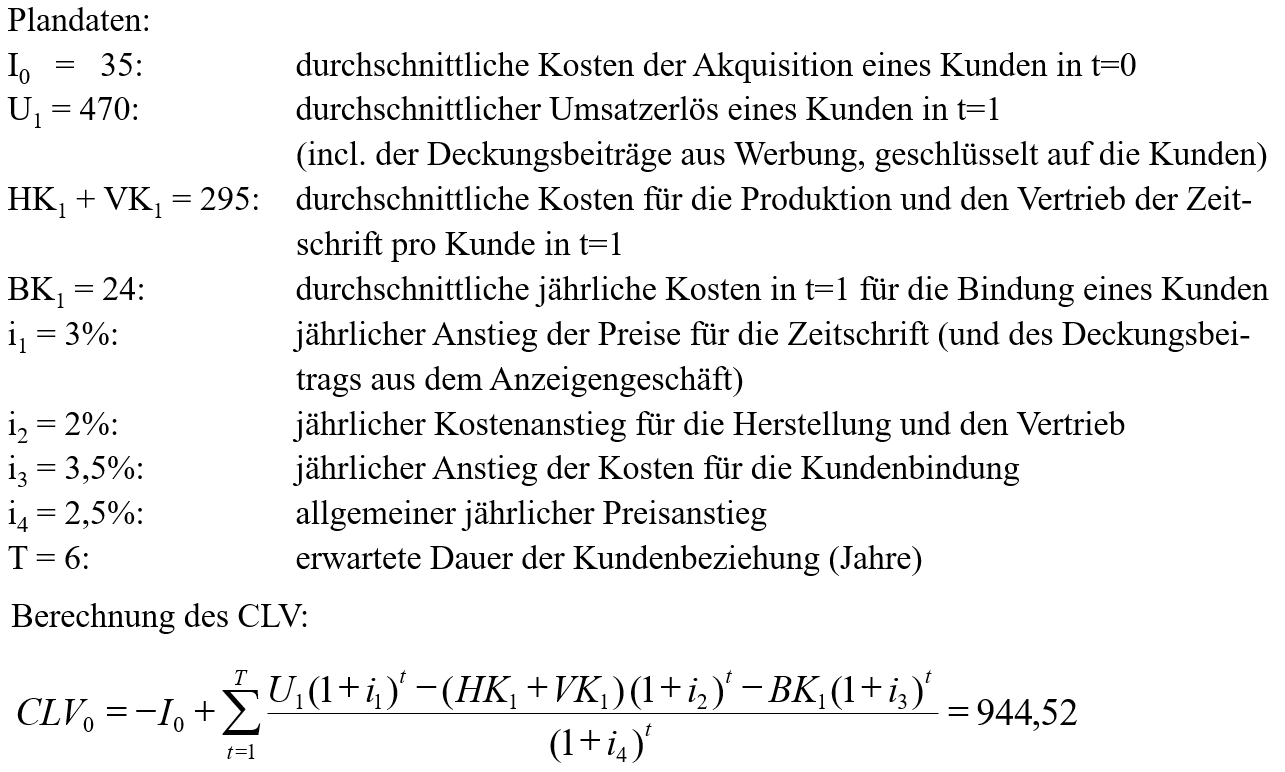
\includegraphics[width=0.8\linewidth]{./images/Marketingcontrolling/CLV4} \end{center}

\end{frame}

\begin{frame}{Idealtypisches Wiederkaufverhalten}
\protect\hypertarget{idealtypisches-wiederkaufverhalten}{}

\begin{center}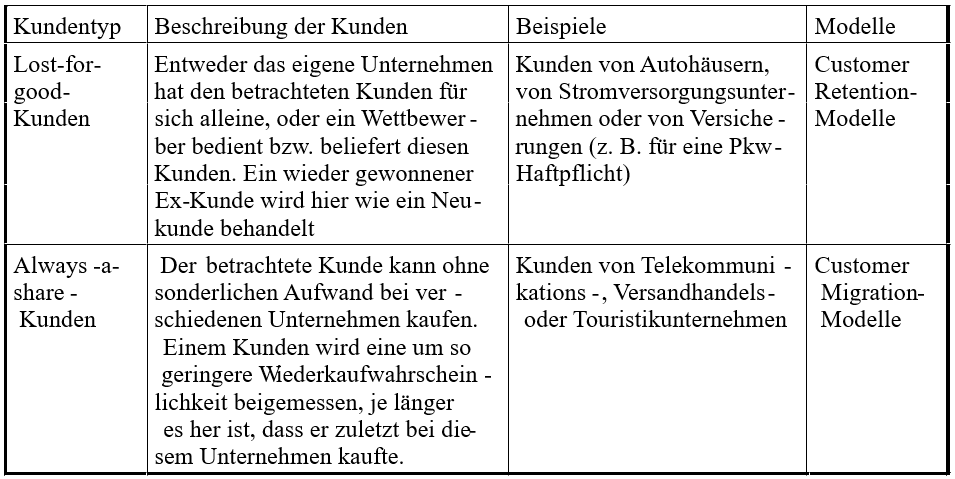
\includegraphics[width=0.8\linewidth]{./images/Marketingcontrolling/CLV5} \end{center}

\end{frame}

\begin{frame}{Formulierung eines Customer Retention-Modells}
\protect\hypertarget{formulierung-eines-customer-retention-modells}{}

\begin{center}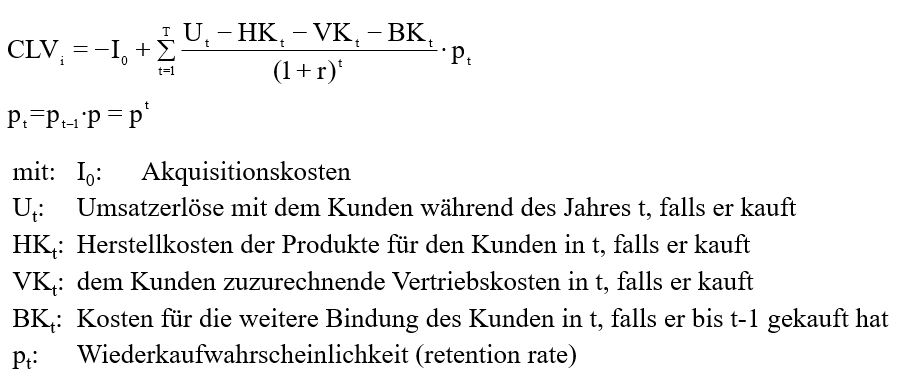
\includegraphics[width=0.8\linewidth]{./images/Marketingcontrolling/CLV6} \end{center}

Anmnerkung:\\
Die Wiederkaufwahrscheinlichkeit in einer bestimmten Periode t
(retention rate) lässt sich aus den Kaufhistorien von bisherigen Kunden
schätzen.

\end{frame}

\hypertarget{strategisches-marketing-controlling}{%
\section{Strategisches Marketing
Controlling}\label{strategisches-marketing-controlling}}

\begin{frame}{Lernziele}
\protect\hypertarget{lernziele-3}{}

\begin{itemize}
\tightlist
\item
  Funktion des strategischen Marketing Controllings verstehen.
\item
  Zusammenhang zwischen Planung und Strategie verstehen.
\item
  Die Bedeutung der Markenstrategi im Rahmend des Marketing-Controllings
  verstehen und evaluieren.
\end{itemize}

\end{frame}

\begin{frame}{Definition Strategie}
\protect\hypertarget{definition-strategie}{}

\begin{quote}
Eine Strategie ist das rational geplante Entscheidungs-, Maßnahmen- und
Verhaltensbündel, das der langfristigen Sicherung des
Unternehmenserfolgs dient.
\end{quote}

\end{frame}

\begin{frame}{Arten von Strategien}
\protect\hypertarget{arten-von-strategien}{}

\begin{center}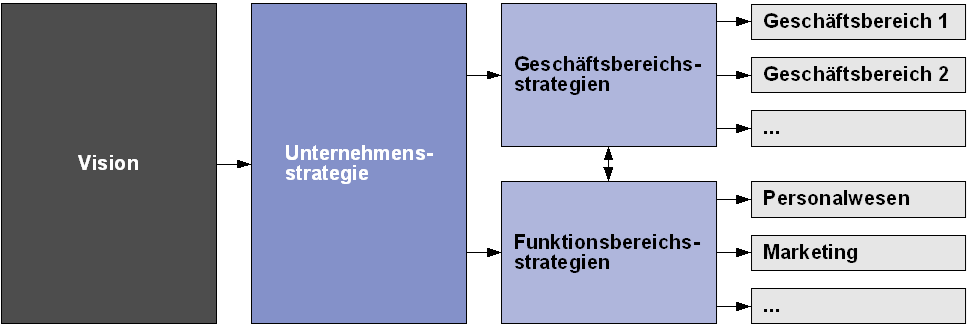
\includegraphics[width=0.8\linewidth]{./images/Marketingcontrolling/Strategiearten} \end{center}

\end{frame}

\begin{frame}[shrink]{Vorgehensweise bei der strategischen Planung}
\protect\hypertarget{vorgehensweise-bei-der-strategischen-planung}{}

\begin{center}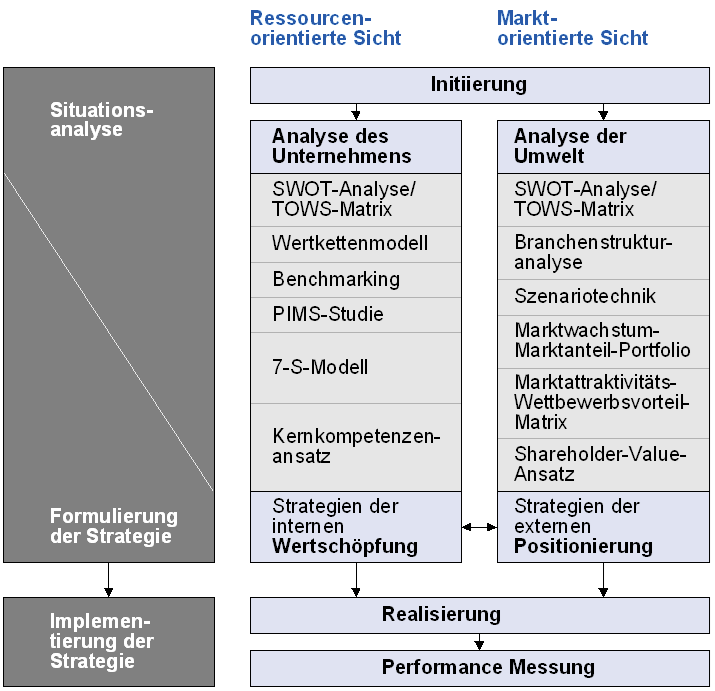
\includegraphics[width=0.8\linewidth]{./images/Marketingcontrolling/Vorgehensweise2} \end{center}

\end{frame}

\begin{frame}{Analyseinstrumente}
\protect\hypertarget{analyseinstrumente}{}

\begin{quote}
Analyseinstrumente dienen dazu, die aus der Unternehmungs- und
Umweltanalye gewonnenen Daten zu verdichten. Mit Hilfe der verschiedenen
Analyseinstrumente gelingt es, die Daten so aufzubereiten, dass sie eine
Grundlage für die Strategiewahl darstellen.
\end{quote}

\end{frame}

\begin{frame}{Übung 12: Strategische Planungsinstrumente}
\protect\hypertarget{ubung-12-strategische-planungsinstrumente}{}

Diskutieren Sie die verschiedenen strategischen Planungsinstrumente aus
der Umwelt- und Unternehmensanalyse. Welche Rolle spielt dabei die
Positionierung und wie könnte diese gemessen werden?

\end{frame}

\begin{frame}{Relevanz des Markenwerts}
\protect\hypertarget{relevanz-des-markenwerts}{}

Der Wert von Marken ist im Wesentlichen darauf zurückzuführen, dass
Marken in der Lage sind, zukünftige Cash-Flows eines Unternehmens zu
beschleunigen, auszuweiten und deren Risiko zu reduzieren:

\begin{itemize}
\tightlist
\item
  Beschleunigung von Cash-Flows, \mbox{z.\thinspace{}B.}\xspace{} durch
  schnellere Reaktion der Konsumenten auf Neuprodukteinführungen infolge
  eines starken Markenimages.
\item
  Ausweitung zukünftiger Cash-Flows durch den Transfer einer etablierten
  Marke auf neue Produktbereiche, Zielgruppen oder Märkte.
\item
  Risikoreduktion zukünftiger Cash-Flows
  \mbox{z.\thinspace{}B.}\xspace{} durch verstärkte Markenloyalität und
  damit erhöhte Wechselkosten bei Einsatz einer starken Marke.
\end{itemize}

\end{frame}

\begin{frame}{Prognose markenspezifischer Zahlungen mit
ertragsorientierten Verfahren}
\protect\hypertarget{prognose-markenspezifischer-zahlungen-mit-ertragsorientierten-verfahren}{}

\textbf{Grundidee}: die zukünftigen Erträge einer Marke,
d.\thinspace{}h. die markenspezifischen Einzahlungsüberschüsse, werden
prognostiziert und auf den Bewertungsstichtag diskontiert.

\textbf{Verfahren}:

\begin{itemize}
\tightlist
\item
  Explizite Prognose markenspezifischer Einzahlungsüberschüsse auf Basis
  einer detaillierten Datenanalyse.
\item
  Einfache pauschalierte Fortschreibung von Zahlungen in die Zukunft.
\end{itemize}

Für die \textbf{Diskontierung} der prognostizierten markenspezifischen
Zahlungsreihen ist ein Kalkulationszinssatz zu bestimmen, der aus
kapitalmarkttheoretischen Modellen abgeleitet werden kann
\mbox{(z.\thinspace{}B.}\xspace{} gemäß dem Capital Asset Pricing Model
(CAPM)).

Ein markenspezifisches Risiko kann dadurch eingebunden werden, dass eine
produktgruppenspezifisch ermittelte Bandbreite von Betafaktoren in
Abhängigkeit der empirisch bestimmten Markenstärke zu einem
markenspezifischen Betafaktor verdichtet wird.

\end{frame}

\begin{frame}{Bewertung markenstrategischer Optionen}
\protect\hypertarget{bewertung-markenstrategischer-optionen}{}

\begin{itemize}
\tightlist
\item
  Auswahl besonders \textbf{erfolgversprechender Transfermärkte}, auf
  welche die zu bewertende Marke zukünftig ausgedehnt werden kann.
\item
  Ermittlung der \textbf{Markentransferpotenzialstärke} dieser Märkte
  über einen so genannten \textbf{Stretching-Score}.
\item
  Der Stretching-Score determiniert die
  \textbf{Erfolgswahrscheinlichkeit} zur Erreichung eines bestimmten
  Marktanteils auf dem Transfermarkt.
\item
  Ermittlung des Stretching-Score über ein
  \textbf{Punktbewertungsverfahren}, in das eine Vielzahl von
  Erfolgsfaktoren von Markentransfers einfließt.
\end{itemize}

\end{frame}

\begin{frame}{Gestaltung des Markenwerts}
\protect\hypertarget{gestaltung-des-markenwerts}{}

\begin{itemize}
\tightlist
\item
  Die wesentliche Ursache dafür, dass Marken einen (finanziellen) Wert
  für Markenanbieter haben, liegt in der Wahrnehmung von Marken durch
  Nachfrager begründet.
\item
  Die Wahrnehmung einer Marke bezieht sich im Wesentlichen auf die
  beiden Konstrukte Markenbekanntheit und Markenimage:

  \begin{itemize}
  \tightlist
  \item
    \textbf{Markenbekanntheit} beinhaltet die Fähigkeit potenzieller
    Nachfrager, ein Markenzeichen zu erinnern oder wieder zu erkennen
    und diese Kenntnisse einer Produktkategorie zuzuordnen.
    Markenbekanntheit ist eine notwendige Bedingung zum Aufbau eines
    Markenimage.
  \item
    \textbf{Markenimage} kann als Wahrnehmungen einer Marke, die in Form
    von Markenassoziationen im Gedächtnis von Nachfragern repräsentiert
    sind, definiert werden. Die Markenassoziationen verkörpern die
    eigentliche inhaltliche Wissensstruktur einer Marke aus der
    subjektiven Sicht von Nachfragern.
  \end{itemize}
\item
  Markenbekanntheit und Markenimage sind die Quelle für zukünftige
  markenspezifische Gewinne und stellen zentrale Treiber des Markenwerts
  dar.
\end{itemize}

\end{frame}

\begin{frame}{Übung 13: Messung des Markenwerts (a)}
\protect\hypertarget{ubung-13-messung-des-markenwerts-a}{}

Viele Unternehmen sind damit befasst, den Wert der Unternehmens-marke
bzw. von Produktmarkten zu messen. Hierfür existieren unterschiedliche
Ansätze, die sich in nicht-monetäre und monetäre Verfahren unterscheiden
lassen.

Stellen Sie sich vor, Sie sind Marketingchef eines bedeutsamen
Konsumgüterherstellers, der eine Vielzahl von einzelnen Produktmarken im
Sortiment führt. Für eines dieser Produkte gilt es, den Markenwert zu
bestimmen.

\textbf{Diskutieren Sie Faktoren, die auf den Markenwert des von Ihnen
betrachteten Konsumguts einwirken.}

\note{Der Wert einer Produktmarke wird durch zahlreiche Faktoren
getrieben. Hierzu zählen beispielsweise die Bekanntheit des Produkts,
die Alleinstellung des Produkts im Absatzmarkt, die Chance, den
Markennamen auf andere Erzeugnisse zu übertragen, die Marge, die dieses
Produkt generiert, die Wettbewerbssituation im Markt, die Investitionen,
die notwendig waren, um die Marke zu generieren.}

\end{frame}

\begin{frame}{Übung 14: Messung des Markenwerts (b)}
\protect\hypertarget{ubung-14-messung-des-markenwerts-b}{}

\textbf{Erörtern Sie die Grenzen des Markenwertkonzepts.}

\note{Die verschiedenen Verfahren zur Erfassung des Markenwertes
gelangen in vielen Anwendungsfällen zu völlig unterschiedlichen Werten
für den Markenwert eine betrachteten Produktes. Abhängig davon, welche
Parameter in die Markenwertbestimmung eingehen, ergeben sich völlig
unterschiedliche Markenwerte. Insofern ist die Diskussion über jene
Faktoren, die markenwerttreibend sind, noch nicht umfassend
abgeschlossen, sodass bislang kein einheitliches Modell zur Erfassung
des Markenwerts vorliegt. Folglich bietet es sich an, verschiedene
Verfahren gleichzeitig einzusetzen, um damit eine Bandbreite für den
Wert einer Marke festzulegen. Neben diesen harten, ökonomischen Werten
bedarf es einer qualitativen, inhaltlichen Diskussion darüber, wie die
verschiedenen Ergebnisse zu interpretieren sind und welche
Schlussfolgerungen sich für die Markenwertgestaltung hieraus ergeben.}

\end{frame}

\hypertarget{conjointanalyse}{%
\section{Conjointanalyse}\label{conjointanalyse}}

\begin{frame}{Lernziele}
\protect\hypertarget{lernziele-4}{}

\begin{itemize}
\tightlist
\item
  Einsatz und Ziel der Conjoint Analyse verstehen.
\item
  Daten für die Conjoint-Analyse aufbereiten.
\item
  Anwendung der Conjoint Analyse.
\item
  Interpretation und Schlussfolgerungen der Conjontanalyse.
\item
  Evaluation des Einsates der Conjoint Analyse in der Marketing
  Controlling Praxis.
\end{itemize}

\end{frame}

\begin{frame}{Einführung Conjointanalyse}
\protect\hypertarget{einfuhrung-conjointanalyse}{}

Häufig stellt sich im operativen Marketing das Problem der Preis- bzw.
Nutzenbestimmung für ein bestimmtes Produkt oder einen
Produktbestandteil. Kunden wägen Angebote gegeneinander ab und
entscheiden sich auf der Basis eines Vergleichs von
Produkteigenschaften, die ihnen wichtig sind, für oder gegen den Kauf.
In der Praxis ist es deshalb sehr wichtig zu wissen, welche
Produkteigenschaften welchen Umfang an Nutzen stiften und wie hoch die
Preisbereitschaft für ein Produkt insgesamt ist.

Typische Fragen, die sich in diesem Zusammenhang stellen, sind

\begin{itemize}
\tightlist
\item
  Welchen Preisaufschlag wird ein Kunde für ein \textbf{Mehr an
  Qualität, Service oder Design} akzeptieren?
\item
  Wie viel ist der Kunde bereit, für eine Sonderausstattung \textbf{mehr
  zu bezahlen}?
\item
  Welcher \textbf{Wert wird einer Anbietermarke} im Vergleich zu den
  Marken der Konkurrenz beigemessen?
\item
  Welche \textbf{Produktmerkmale} sind für Kunden essenziell, welche
  hingegen zweitrangig?
\end{itemize}

\end{frame}

\begin{frame}{Probleme der Informationsbeschaffung durch direkte
Befragung}
\protect\hypertarget{probleme-der-informationsbeschaffung-durch-direkte-befragung}{}

\begin{itemize}
\tightlist
\item
  Wert einzelener Merkmale schwer zu quantifizieren
\item
  Gefahr unehrlicher Antworten (bei Preisbereitschaft)
\item
  Keine Abwägung zwischen Nutzen und Kostenm, wenn Preis im Fokus.
\end{itemize}

\end{frame}

\begin{frame}{Einsatz von Conjointanalysen}
\protect\hypertarget{einsatz-von-conjointanalysen}{}

\begin{itemize}
\item
  Conjoint-Analysen werden in der Praxis vorwiegend bei der
  \textbf{Preisfestsetzung}, der \textbf{Neuproduktplanung} und für die
  \textbf{Nachfragersegmentierung} eingesetzt.
\item
  Sie gelten im Vergleich zu anderen Verfahren durch die indirekte
  Datenerhebung als \textbf{realitätsnahe Form} der Präferenzmessung mit
  einer höheren Validität als andere Verfahren.
\item
  Bei der Conjoint-Analyse werden, je nach Vorgehen, ein oder mehrere
  Produktkonzepte zur Einschätzung einer Stichprobe von
  Auskunftspersonen vorgelegt.
\item
  Die Produkte werden dabei durch Merkmale definiert, die ein bestimmtes
  Set an Ausprägungen besitzen.
\item
  Somit identifiziert die Auskunftsperson \textbf{Teilnutzenwerte} für
  jede Merkmalsausprägung.
\item
  So kann aufgrund der gemessenen Präferenzen eine Prognose erstellen
  werden, welches Produkt eine Auskunftsperson bevorzugt und in Zukunft
  wahrscheinlich kaufen wird.
\end{itemize}

\end{frame}

\begin{frame}{Zielsetzung von Conjointanalysen}
\protect\hypertarget{zielsetzung-von-conjointanalysen}{}

Zielsetzung von Conjoint-Analysen im Falle von Präferenzprognosen sind
die \textbf{Vorhersage zukünftiger Kaufentscheidungen}.

\begin{itemize}
\tightlist
\item
  Um diese Vorhersagen zu berechnen, können
  \textbf{Kaufentscheidungsmodelle} angewendet werden.
\item
  Dabei werden für verschiedene hypothetische Produktalternativen
  \textbf{Gesamtnutzenwerte} geschätzt, die anschließend in
  Auswahlwahrscheinlichkeiten transformiert werden.
\item
  Bei allen Modellen erfolgt die Wahlentscheidung nach dem
  \textbf{Nutzenmaximierungsprinzip}, so dass Alternativen mit höherem
  Nutzen solchen Alternativen mit niedrigerem Nutzen vorgezogen werden.
\end{itemize}

\end{frame}

\begin{frame}{Modelle der Nutzenschätzung}
\protect\hypertarget{modelle-der-nutzenschatzung}{}

\begin{itemize}
\tightlist
\item
  \textbf{Max Utility-Modell}: Die Alternative mit dem höchsten
  Gesamtnutzen bekommt die Wahlwahrscheinlichkeit 1. Alle anderen
  Alternativen bekommen die Wahlwahrscheinlichkeit 0. Bei mehreren
  Alternativen mit dem gleichen Gesamtnutzen wird die
  Wahlwahrscheinlichkeit gleich verteilt.
\item
  \textbf{BTL-Modell} (nach Bradley, Terry und Luce): Die
  Wahlwahrscheinlichkeit errechnet sich aus dem Quotient von
  Gesamtnutzen einer Alternative und der Summe der Gesamtnutzen aller
  Alternativen.
\item
  \textbf{Logit-Modell}: Für jede Alternative wird nicht der
  Gesamtnutzen, sondern der e-transformierte Gesamtnutzen (Eulersche
  Zahl e = 2,718281828459045235\ldots{}) der Alternative berechnet. Die
  Wahlwahrscheinlichkeit errechnet sich dann aus dem Quotient von
  e-transformiertem Gesamtnutzen einer Alternative und der Summe der
  e-transformierten Gesamtnutzen aller Alternativen.
\end{itemize}

\end{frame}

\begin{frame}{Nachteil von Entscheidungsmodellen}
\protect\hypertarget{nachteil-von-entscheidungsmodellen}{}

Die Nutzung solcher Entscheidungsmodelle für Prognosezwecke ist dann
\textbf{problematisch}, wenn keine Informationen über die realen
Kaufentscheidungprozesse der Konsumenten vorliegen.

Der Marktforscher müsste sich für seine Prognosen folglich für eines der
Entscheidungsmodelle entscheiden. Da in den seltensten Fällen mit
gleichen Wahlwahrscheinlichkeiten bei den Auskunftspersonen zu rechnen
ist, führt die Modellauswahl zwangsläufig zu einer Prognose, die
individuell vom Marktforscher durch seine Auswahl beeinflusst wird.
Dieser Nachteil besteht bei der Gruppe der \textbf{traditionellen
Conjoint-Analysen}, bei denen die beurteilten Alternativen in eine
Präferenzrangfolge der Auskunftsperson gebracht werden oder mittels
Rating-Skalen bewertet

\end{frame}

\begin{frame}{Choice-Based Conjoint-Analysen}
\protect\hypertarget{choice-based-conjoint-analysen}{}

Bei Choice-Based Conjoint-Analysen werden den Auskunftspersonen
verschiedenen \textbf{Choice-Sets} angeboten, aus der sie jeweils die
für sie attraktivste Alternative auswählen.

Ein \textbf{Choice-Set} besteht dabei aus zwei \textbf{hypothetischen
Auswahl-Alternativen} und der Möglichkeit der \textbf{Nichtwahl}, also
die Wahl keiner der Alternativen. Diese letzte Option gewährleistet bei
der Nutzenschätzung, dass nur kaufrelevante Alternativen in die
Berechnung eingehen. So kann vermutet werden, dass bei der der
Choice-Based Conjoint-Analyse das natürliche Kaufverhalten der
Auskunftsperson analysiert wird.

Dabei werden aus Präferenzen (Gesamtnutzen) die
\textbf{Präferenzbeiträge (Teilnutzen)} der einzelnen
Merkmalsausprägungen geschätzt, wobei die Beurteilungsobjekte auf der
Grundlage experimenteller Designs konstruiert werden

\end{frame}

\begin{frame}{Prozess der Choice-Based Conjoint-Analysen}
\protect\hypertarget{prozess-der-choice-based-conjoint-analysen}{}

\begin{enumerate}
\tightlist
\item
  Charakterisierung des Entscheidungsprozesses
\item
  Identifizieren und Beschreiben der Merkmale
\item
  Entwicklung eines experimentellen Design
\item
  Entwicklung des Fragebogen
\item
  Sammeln der Daten
\item
  Schätzmodell
\item
  Interpretation der Ergebnisse zur Entscheidungsunterstützung
\end{enumerate}

\end{frame}

\begin{frame}{Übung 15: Anforderungen an Auswahl der Merkmale}
\protect\hypertarget{ubung-15-anforderungen-an-auswahl-der-merkmale}{}

Welchen Aussagen stimmen Sie zu?

\begin{enumerate}
[A.]
\tightlist
\item
  Die Merkmale müssen für die Kaufentscheidung nicht relevant sein.
\item
  Die Anzahl der Merkmale sollt möglichst hoch sein.
\item
  Die Auskunftspersonen können überfordert werden.
\item
  Die Merkmale sollten einen direkten Einfluss auf den Gesamtnutzen der
  Alternative haben.
\item
  Die Merkmale sollten unabhängig voneinander und damit nicht redundant
  sein.
\item
  Die Merkmale sollten vom Unternehmen beeinflussbar und realisierbar
  sein.
\item
  Die Formulierung der Merkmale und Merkmalsausprägungen sollte objektiv
  und ohne Interpretationsspielraum sein.
\item
  Aus den definierten Merkmalen und Ausprägungen sollten realistischen
  Alternativkonzepte möglich sein.
\end{enumerate}

\note{\textbf{D-E sind richtig}}

\end{frame}

\begin{frame}{Übung 16: Anforderungen an die Merkamalsausprägungen}
\protect\hypertarget{ubung-16-anforderungen-an-die-merkamalsauspragungen}{}

Welchen Aussagen stimmen Sie zu?

\begin{enumerate}
[A.]
\tightlist
\item
  Die Entscheidungssituation muss durch die Ausprägungen realistisch
  abgebildet werden.
\item
  Die Ausprägungen müssen nicht unbedingt einen Nutzenbeitrag zur
  Präferenzbildung leisten.
\item
  Die Anzahl der Ausprägungen je Merkmal sollte möglichst hoch sein.
\item
  Die Ausprägungen sollten vollständig sein und sich gegenseitig
  ausschließen.
\end{enumerate}

\note{\textbf{A, C und D sind richtig}}

\end{frame}

\begin{frame}{Fallstudie}
\protect\hypertarget{fallstudie}{}

Als Fallstudie dient das Produkt „Digitale Lernform`` im Rahmen der
beruflichen Weiterbildung. Die Studie wurde bei 172 Probanden aus
Teilnehmern der TÜV SÜD Akademie im Bereich der beruflichen
Weiterbildung in dem Zeitraum von 01.02.2014 bis 31.03.2014
durchgeführt.

Quelle:

Gansser, O.; Füller, S.\thinspace{}R. (2015): Präferenzprognosen mittels
Conjoint-Analyse - eine Fallstudie mit Choice-Based-Design, in: Gansser,
O.; Krol, B. (Hrsg.): Markt- und Absatzprognosen, Wiesbaden.

\end{frame}

\begin{frame}{Merkmale und Beschreibung der Merkmalsausprägungen}
\protect\hypertarget{merkmale-und-beschreibung-der-merkmalsauspragungen}{}

\begin{center}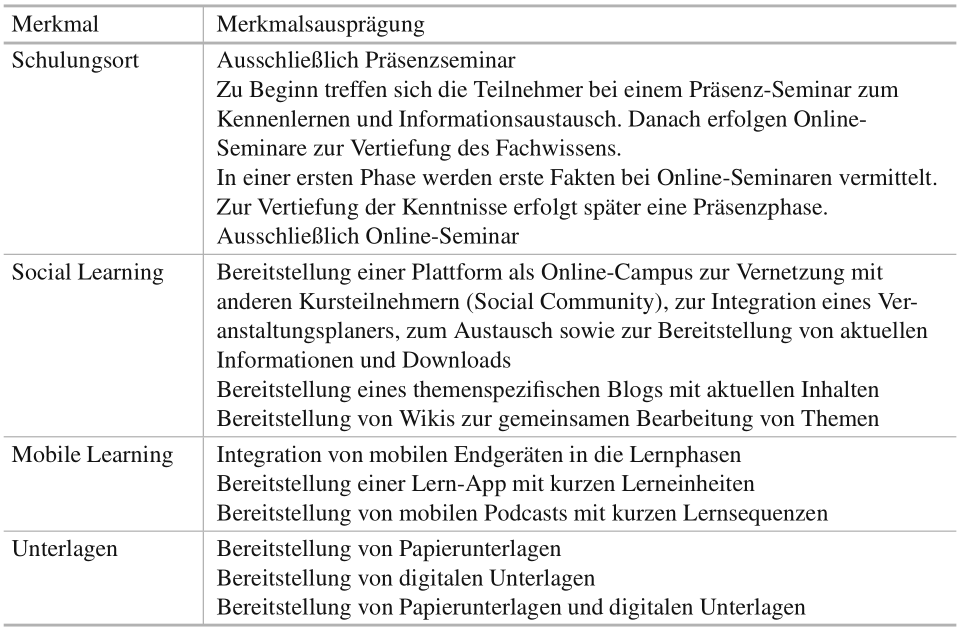
\includegraphics[width=0.8\linewidth]{./images/Marketingcontrolling/Merkmale} \end{center}

\end{frame}

\begin{frame}{Merkmale und Beschreibung der Merkmalsausprägungen}
\protect\hypertarget{merkmale-und-beschreibung-der-merkmalsauspragungen-1}{}

\begin{center}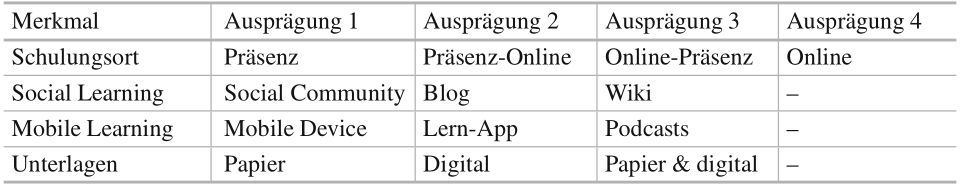
\includegraphics[width=0.8\linewidth]{./images/Marketingcontrolling/Kurznotation} \end{center}

\end{frame}

\begin{frame}{Erstellung orthogonal fraktionierter Choice-Sets mit der
Statistik-Software R}
\protect\hypertarget{erstellung-orthogonal-fraktionierter-choice-sets-mit-der-statistik-software-r}{}

Schritte:

\begin{enumerate}
\tightlist
\item
  Erstellung eines \textbf{vollständigen Designs},
\item
  Erstellung eines \textbf{fraktionierten Designs} mit orthogonaler
  Anordnung,
\item
  Kopieren des fraktionierten Designs von Auswahlalternative 1 für das
  Design der Auswahlalternative 2,
\item
  Erstellung von finalen Choice-Sets mit Hilfe von Zufallszahlen.
\end{enumerate}

\end{frame}

\begin{frame}[fragile]{1 Erzeugung eines vollständigen Designs}
\protect\hypertarget{erzeugung-eines-vollstandigen-designs}{}

Bei der vorliegenden Fallstudie beinhaltet ein vollständiges Design
\textbf{4x3x3x3 Kombinationsmöglichkeiten}, da ein Merkmal vier
Ausprägungen und drei Merkmalen drei Ausprägungen umfasst.

Für die Erstellung des vollständigen Design wird über die Funktion
\textbf{gen.factorial} ein \textbf{4x3x3x3 Design} mit den
Variablenbezeichnungen \textbf{``Ort'', ``SL'', ``ML'' und ``Unt''} und
dem Argument, dass alle Variablen Faktoren, mit nominaler Ausprägung
sind, eine Matrix mit der Bezeichnung \textbf{vd} (vollständiges Design)
erzeugt.

Code:

\begin{Shaded}
\begin{Highlighting}[]
\KeywordTok{library}\NormalTok{(AlgDesign)}
\NormalTok{vd <-}\StringTok{ }\KeywordTok{gen.factorial}\NormalTok{(}\KeywordTok{c}\NormalTok{(}\DecValTok{4}\NormalTok{,}\DecValTok{3}\NormalTok{,}\DecValTok{3}\NormalTok{,}\DecValTok{3}\NormalTok{), }
                    \DataTypeTok{varNames=}\KeywordTok{c}\NormalTok{(}\StringTok{"Ort"}\NormalTok{, }\StringTok{"SL"}\NormalTok{, }\StringTok{"ML"}\NormalTok{, }\StringTok{"Unt"}\NormalTok{), }
                    \DataTypeTok{factors=}\StringTok{"all"}\NormalTok{)}
\end{Highlighting}
\end{Shaded}

\end{frame}

\begin{frame}[fragile]{Ausgabe des vollständigen Designs (esten 16
Zeilen)}
\protect\hypertarget{ausgabe-des-vollstandigen-designs-esten-16-zeilen}{}

\begin{verbatim}
##    Ort SL ML Unt
## 1    1  1  1   1
## 2    2  1  1   1
## 3    3  1  1   1
## 4    4  1  1   1
## 5    1  2  1   1
## 6    2  2  1   1
## 7    3  2  1   1
## 8    4  2  1   1
## 9    1  3  1   1
## 10   2  3  1   1
## 11   3  3  1   1
## 12   4  3  1   1
## 13   1  1  2   1
## 14   2  1  2   1
## 15   3  1  2   1
## 16   4  1  2   1
\end{verbatim}

\end{frame}

\begin{frame}[fragile]{Ausgabe des vollständigen Designs (letzte 16
Zeilen)}
\protect\hypertarget{ausgabe-des-vollstandigen-designs-letzte-16-zeilen}{}

\begin{verbatim}
##     Ort SL ML Unt
## 92    4  2  2   3
## 93    1  3  2   3
## 94    2  3  2   3
## 95    3  3  2   3
## 96    4  3  2   3
## 97    1  1  3   3
## 98    2  1  3   3
## 99    3  1  3   3
## 100   4  1  3   3
## 101   1  2  3   3
## 102   2  2  3   3
## 103   3  2  3   3
## 104   4  2  3   3
## 105   1  3  3   3
## 106   2  3  3   3
## 107   3  3  3   3
## 108   4  3  3   3
\end{verbatim}

\end{frame}

\begin{frame}[fragile]{2 Erstellung eines fraktionierten Designs mit
orthogonaler Anordnung}
\protect\hypertarget{erstellung-eines-fraktionierten-designs-mit-orthogonaler-anordnung}{}

\begin{Shaded}
\begin{Highlighting}[]
\KeywordTok{set.seed}\NormalTok{(}\DecValTok{1986}\NormalTok{) }\CommentTok{# Initialisierung eines Zufallsgeneraturs}
\NormalTok{fd <-}\StringTok{ }\KeywordTok{optFederov}\NormalTok{(}\OperatorTok{~}\NormalTok{.,vd,}\DecValTok{16}\NormalTok{) }\CommentTok{# Erstellung eines fraktionierten Designs }
                           \CommentTok{# mit 16 Alternativzeilen}
\NormalTok{alt1 <-}\StringTok{ }\NormalTok{fd}\OperatorTok{$}\NormalTok{design  }\CommentTok{# Zuweisung des Designs zu einer Matrix alt1 }
\end{Highlighting}
\end{Shaded}

\end{frame}

\begin{frame}[fragile]{Ausgabe von alt1}
\protect\hypertarget{ausgabe-von-alt1}{}

\begin{verbatim}
##     Ort SL ML Unt
## 4     4  1  1   1
## 5     1  2  1   1
## 19    3  2  2   1
## 26    2  1  3   1
## 36    4  3  3   1
## 47    3  3  1   2
## 49    1  1  2   2
## 58    2  3  2   2
## 65    1  2  3   2
## 68    4  2  3   2
## 76    4  1  1   3
## 78    2  2  1   3
## 92    4  2  2   3
## 93    1  3  2   3
## 99    3  1  3   3
## 105   1  3  3   3
\end{verbatim}

\end{frame}

\begin{frame}[fragile]{3 Kopieren des fraktionierten Designs von alt1
für alt2}
\protect\hypertarget{kopieren-des-fraktionierten-designs-von-alt1-fur-alt2}{}

Da die Probanden bei der Choice-Based Conjoint-Analyse bei jeder
Auswahlentscheidung zwischen zwei Auswahlalternativen entscheiden
müssen, wird das fraktionierte Design der Auswahlalternative 1 in eine
zweite Matrix geschrieben, die der Matrix alt2 zugewiesen wird.

Somit sind nun zwei identische fraktionierte Designs (alt1 und alt2) als
Matrix vorhanden.

Code:

\begin{Shaded}
\begin{Highlighting}[]
\NormalTok{alt2 <-}\StringTok{ }\NormalTok{alt1}
\end{Highlighting}
\end{Shaded}

\end{frame}

\begin{frame}[fragile]{4 Erstellung von finalen Choice-Sets}
\protect\hypertarget{erstellung-von-finalen-choice-sets}{}

Beiden Matrizen Zufallszahlen werden je Zeile generiert, die in eine
weitere Spalte z (Zufallszahl) je Matrix geschrieben werden. Beide
Matrizen werden in einem letzten Schritt auf Basis der je Zeile
zugeordneten Zufallszahlen mit dem Argument „order`` aufsteigend
sortiert.

\begin{Shaded}
\begin{Highlighting}[]
\NormalTok{alt1 <-}\StringTok{ }\KeywordTok{transform}\NormalTok{(alt1,}\DataTypeTok{z1=}\KeywordTok{runif}\NormalTok{(}\DecValTok{16}\NormalTok{))}
\NormalTok{alt2 <-}\StringTok{ }\KeywordTok{transform}\NormalTok{(alt2,}\DataTypeTok{z2=}\KeywordTok{runif}\NormalTok{(}\DecValTok{16}\NormalTok{))}
\NormalTok{alt1_sort <-}\StringTok{ }\NormalTok{alt1[}\KeywordTok{order}\NormalTok{(alt1}\OperatorTok{$}\NormalTok{z1),]}
\NormalTok{alt2_sort <-}\StringTok{ }\NormalTok{alt2[}\KeywordTok{order}\NormalTok{(alt2}\OperatorTok{$}\NormalTok{z2),]}
\end{Highlighting}
\end{Shaded}

Sollten eine oder mehrere Zeilen gleiche Stimuli aufweisen, muss der
Schritt 4 so oft wiederholt werden, bis jedes Choice-Set aus
unterschiedlichen Stimuli besteht.

\end{frame}

\begin{frame}[fragile]{Ausgabe Choice-Set 1 als Beispiel}
\protect\hypertarget{ausgabe-choice-set-1-als-beispiel}{}

\begin{verbatim}
##     Ort SL ML Unt         z1
## 99    3  1  3   3 0.00836387
## 26    2  1  3   1 0.13044868
## 78    2  2  1   3 0.22792301
## 93    1  3  2   3 0.41081482
## 5     1  2  1   1 0.45177166
## 68    4  2  3   2 0.53615863
## 92    4  2  2   3 0.63137372
## 105   1  3  3   3 0.65178508
## 36    4  3  3   1 0.75591259
## 76    4  1  1   3 0.77781755
## 47    3  3  1   2 0.80663708
## 19    3  2  2   1 0.86051224
## 58    2  3  2   2 0.86860922
## 49    1  1  2   2 0.88878604
## 4     4  1  1   1 0.91496675
## 65    1  2  3   2 0.92896275
\end{verbatim}

\end{frame}

\begin{frame}[fragile]{Einlesen der Original Choice-Sets aus Projekt}
\protect\hypertarget{einlesen-der-original-choice-sets-aus-projekt}{}

Da die Zufallsinitionalisierung für diese Conjointanalyse 2014
durchgeführt wurde, werden bei erneuter Fraktionierung andere Zeilen
ausgewählt als dies 2014 der Fall war. Aus diesem Grunde werden beiden
Choice-Sets zum Download zur Verfügung gestellt.

Code:

\begin{Shaded}
\begin{Highlighting}[]
\KeywordTok{load}\NormalTok{(}\KeywordTok{url}\NormalTok{(}\StringTok{"http://gansser.de/data/conjoint/alt1_o.Rdata"}\NormalTok{))}
\KeywordTok{load}\NormalTok{(}\KeywordTok{url}\NormalTok{(}\StringTok{"http://gansser.de/data/conjoint/alt2_o.Rdata"}\NormalTok{))}
\end{Highlighting}
\end{Shaded}

\end{frame}

\begin{frame}[fragile,shrink]{Ausgabe Original Choice-Set 1 mir
Recodierung}
\protect\hypertarget{ausgabe-original-choice-set-1-mir-recodierung}{}

\begin{Shaded}
\begin{Highlighting}[]
\NormalTok{alt1_o}
\end{Highlighting}
\end{Shaded}

\begin{verbatim}
##      X               Ort               SL                  ML
## 1   33        Pr\xe4senz             Wiki             Podcast
## 2   15 Online-Pr\xe4senz Online.Community            Lern-App
## 3   22 Pr\xe4senz-Online             Wiki            Lern-App
## 4    8            Online             Blog Mobile.Endger\xe4te
## 5   47 Online-Pr\xe4senz             Wiki Mobile.Endger\xe4te
## 6   89        Pr\xe4senz             Blog            Lern-App
## 7   45        Pr\xe4senz             Wiki Mobile.Endger\xe4te
## 8   66 Pr\xe4senz-Online             Blog             Podcast
## 9  103 Online-Pr\xe4senz             Blog             Podcast
## 10  64            Online Online.Community             Podcast
## 11  56            Online             Blog            Lern-App
## 12  96            Online             Wiki            Lern-App
## 13  49        Pr\xe4senz Online.Community            Lern-App
## 14  74 Pr\xe4senz-Online Online.Community Mobile.Endger\xe4te
## 15 100            Online Online.Community             Podcast
## 16   1        Pr\xe4senz Online.Community Mobile.Endger\xe4te
##                   Unt          z1
## 1              Papier 0.006721412
## 2              Papier 0.024326878
## 3              Papier 0.026332645
## 4              Papier 0.200443716
## 5             Digital 0.269644150
## 6  Papier.und.Digital 0.552909261
## 7             Digital 0.591650470
## 8             Digital 0.597378352
## 9  Papier.und.Digital 0.695849171
## 10            Digital 0.706909481
## 11            Digital 0.758686919
## 12 Papier.und.Digital 0.798375591
## 13            Digital 0.876851384
## 14 Papier.und.Digital 0.877162066
## 15 Papier.und.Digital 0.936571233
## 16             Papier 0.991988726
\end{verbatim}

\end{frame}

\begin{frame}[fragile,shrink]{Ausgabe Original Choice-Set 2 mir
Recodierung}
\protect\hypertarget{ausgabe-original-choice-set-2-mir-recodierung}{}

\begin{Shaded}
\begin{Highlighting}[]
\NormalTok{alt2_o}
\end{Highlighting}
\end{Shaded}

\begin{verbatim}
##      X               Ort               SL                  ML
## 1   56            Online             Blog            Lern-App
## 2  100            Online Online.Community             Podcast
## 3   47 Online-Pr\xe4senz             Wiki Mobile.Endger\xe4te
## 4   96            Online             Wiki            Lern-App
## 5   66 Pr\xe4senz-Online             Blog             Podcast
## 6   49        Pr\xe4senz Online.Community            Lern-App
## 7   15 Online-Pr\xe4senz Online.Community            Lern-App
## 8   89        Pr\xe4senz             Blog            Lern-App
## 9    1        Pr\xe4senz Online.Community Mobile.Endger\xe4te
## 10  74 Pr\xe4senz-Online Online.Community Mobile.Endger\xe4te
## 11  64            Online Online.Community             Podcast
## 12   8            Online             Blog Mobile.Endger\xe4te
## 13  33        Pr\xe4senz             Wiki             Podcast
## 14  22 Pr\xe4senz-Online             Wiki            Lern-App
## 15  45        Pr\xe4senz             Wiki Mobile.Endger\xe4te
## 16 103 Online-Pr\xe4senz             Blog             Podcast
##                   Unt         z2
## 1             Digital 0.01468773
## 2  Papier.und.Digital 0.07356267
## 3             Digital 0.09334121
## 4  Papier.und.Digital 0.14596041
## 5             Digital 0.16373591
## 6             Digital 0.43730748
## 7              Papier 0.45675145
## 8  Papier.und.Digital 0.54972278
## 9              Papier 0.64408133
## 10 Papier.und.Digital 0.70464075
## 11            Digital 0.74790253
## 12             Papier 0.76833706
## 13             Papier 0.87132066
## 14             Papier 0.89802574
## 15            Digital 0.92317763
## 16 Papier.und.Digital 0.98235841
\end{verbatim}

\end{frame}

\begin{frame}{Präsentation der Stimuli bei den Befragungsteilnehmern}
\protect\hypertarget{prasentation-der-stimuli-bei-den-befragungsteilnehmern}{}

\begin{center}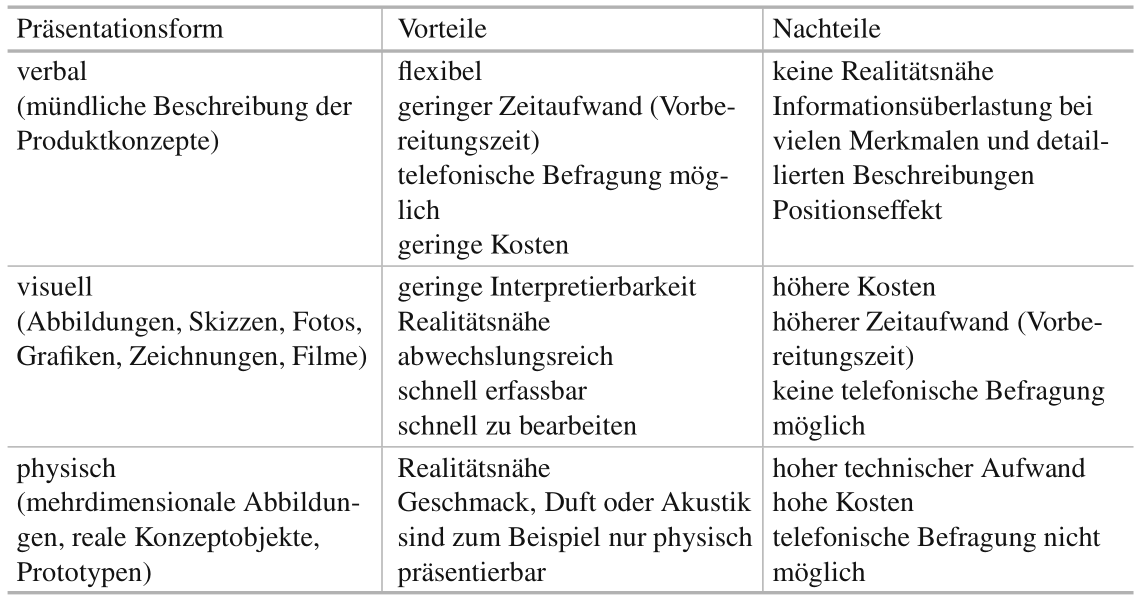
\includegraphics[width=0.8\linewidth]{./images/Marketingcontrolling/Stimuli} \end{center}

\end{frame}

\begin{frame}{Vorlage Choice-Set 1}
\protect\hypertarget{vorlage-choice-set-1}{}

\begin{center}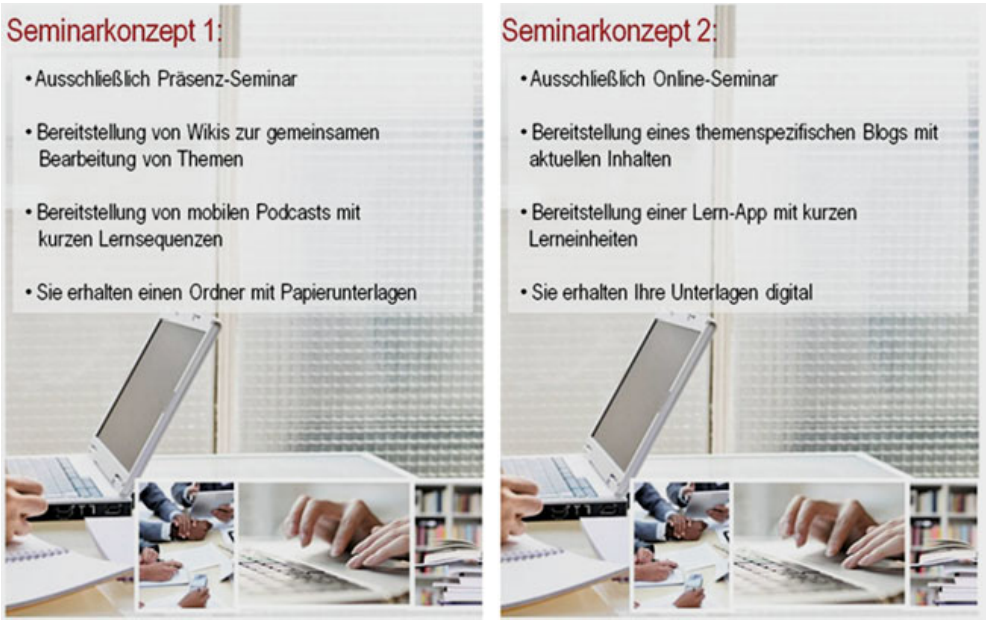
\includegraphics[width=0.8\linewidth]{./images/Marketingcontrolling/Choice-Set1} \end{center}

\end{frame}

\begin{frame}{Dateneingabe}
\protect\hypertarget{dateneingabe}{}

Von jeder Auskunftsperson liegen 16 Entscheidungen zwischen
\textbf{Alternative 1}, \textbf{Alternative 2} oder \textbf{„Ich wähle
keines der beiden Konzepte``} vor.

Diese Informationen müssen nun in eine Datenmatrix geschrieben werden,
die in einem nächsten Schritt als Dateninput für die Nutzenfunktion
verwendet wird.

\end{frame}

\begin{frame}[fragile,shrink]{Einlesen der Daten}
\protect\hypertarget{einlesen-der-daten}{}

\begin{Shaded}
\begin{Highlighting}[]
\KeywordTok{load}\NormalTok{(}\KeywordTok{url}\NormalTok{(}\StringTok{"http://gansser.de/data/conjoint/conjoint_data.Rdata"}\NormalTok{))}
\NormalTok{conjoint_data[}\DecValTok{1}\OperatorTok{:}\DecValTok{12}\NormalTok{,] }\CommentTok{# Output der Daten für die ersten vier Personen}
\end{Highlighting}
\end{Shaded}

\begin{verbatim}
##    APN E K                  Ort             SL             ML
## 1  101 0 1        A1 Pr\xe4senz        A3 Wiki    A3 Podcasts
## 2  101 1 1            A4 Online        A2 Blog    A2 Lern-App
## 3  101 0 0                    0              0              0
## 4  102 0 1 A3 Online-Pr\xe4senz A1 Social Com.    A2 Lern-App
## 5  102 1 1            A4 Online A1 Social Com.    A3 Podcasts
## 6  102 0 0                    0              0              0
## 7  103 0 1 A2 Pr\xe4senz-Online        A3 Wiki    A2 Lern-App
## 8  103 1 1 A3 Online-Pr\xe4senz        A3 Wiki A1 Mobile Dev.
## 9  103 0 0                    0              0              0
## 10 104 0 1            A4 Online        A2 Blog A1 Mobile Dev.
## 11 104 1 1            A4 Online        A3 Wiki    A2 Lern-App
## 12 104 0 0                    0              0              0
##                    Unt
## 1            A1 Papier
## 2           A2 Digital
## 3                    0
## 4            A1 Papier
## 5  A3 Papier & Digital
## 6                    0
## 7            A1 Papier
## 8           A2 Digital
## 9                    0
## 10           A1 Papier
## 11 A3 Papier & Digital
## 12                   0
\end{verbatim}

\end{frame}

\begin{frame}{Erklärung der Dateneingabematrix}
\protect\hypertarget{erklarung-der-dateneingabematrix}{}

Die Spalte APN setzt sich zusammen aus der Nummer der Auskunftsperson
und der Nummer des Choice-Sets.

Am Beispiel der ersten Auskunftsperson bedeuten die ersten drei Ziffern
die Auskunftsperson Nr. 1 und die letzten zwei Ziffern, dass es sich um
das erste, zweite, drieet und vierte Choice-Set im Fragebogen handelt.

In der Spalte E wird die \textbf{Entscheidung der Probanden}
gespeichert.

\begin{itemize}
\tightlist
\item
  Steht in der Zelle eine 1, dann wurde das in dieser Zeile definierte
  Choice-Set gewählt.
\item
  Andernfalls enthält die Zelle eine 0 für die Nicht-Wahl.
\end{itemize}

Pro Choice-Set gibt es genau drei Zeilen.

\begin{itemize}
\tightlist
\item
  Die erste Zeile jeweils für die Ausprägungen von \textbf{Alternative
  1},
\item
  die zweite Zeile jeweils für die \textbf{Alternative 2} und die
\item
  dritte Zeile für die \textbf{Nicht-Auswahl}.
\end{itemize}

Bei der Spalte K handelt es sich um die spezifische Alternativkonstante,
bei der die Ziffer 1 eine Auswahlalternative darstellt und die Ziffer 0
die Nicht-Auswahl.

\end{frame}

\begin{frame}{Schätzung der Nutzenfunktion}
\protect\hypertarget{schatzung-der-nutzenfunktion}{}

Zur Schätzung der \textbf{Nutzenfunktion} für Choice-Based
Conjoint-Analysen mit mehr als zwei Alternativen stellt das Verfahren
der Multinomialen Logit-Analyse das wichtigste Verfahren dar.

Mit dem Paket „survival`` wird in R mit der Funktion clogit () ein
konditionales \textbf{Logit-Modell} angewendet.

Dabei wird die \textbf{Wahrscheinlichkeit} errechnet, mit der eine
gezeigte Produktalternative gewählt wird

\end{frame}

\begin{frame}[fragile,shrink]{Code für die Nutzenschätzung}
\protect\hypertarget{code-fur-die-nutzenschatzung}{}

\begin{Shaded}
\begin{Highlighting}[]
\KeywordTok{library}\NormalTok{(survival) }\CommentTok{# Paket vorher installieren mit install.packages("")}
\NormalTok{clogout <-}\StringTok{ }\KeywordTok{clogit}\NormalTok{(E}\OperatorTok{~}\NormalTok{K}\OperatorTok{+}\NormalTok{Ort}\OperatorTok{+}\NormalTok{SL}\OperatorTok{+}\NormalTok{ML}\OperatorTok{+}\NormalTok{Unt}\OperatorTok{+}\KeywordTok{strata}\NormalTok{(APN), }\DataTypeTok{data=}\NormalTok{conjoint_data)}
\NormalTok{clogout}
\end{Highlighting}
\end{Shaded}

\begin{verbatim}
## Call:
## clogit(E ~ K + Ort + SL + ML + Unt + strata(APN), data = conjoint_data)
## 
##                            coef exp(coef) se(coef)      z       p
## K                       -0.2031    0.8162   0.0940  -2.16  0.0306
## OrtA1 Pr\xe4senz         1.7357    5.6726   0.1029  16.88 < 2e-16
## OrtA2 Pr\xe4senz-Online  1.5758    4.8347   0.1045  15.08 < 2e-16
## OrtA3 Online-Pr\xe4senz  1.6455    5.1836   0.0937  17.55 < 2e-16
## OrtA4 Online                 NA        NA   0.0000     NA      NA
## SLA1 Social Com.         0.3188    1.3754   0.0684   4.66 3.2e-06
## SLA2 Blog               -0.1405    0.8689   0.0832  -1.69  0.0914
## SLA3 Wiki                    NA        NA   0.0000     NA      NA
## MLA1 Mobile Dev.        -0.2469    0.7812   0.0781  -3.16  0.0016
## MLA2 Lern-App            0.0848    1.0885   0.0688   1.23  0.2178
## MLA3 Podcasts                NA        NA   0.0000     NA      NA
## UntA1 Papier            -0.6116    0.5425   0.0697  -8.77 < 2e-16
## UntA2 Digital           -0.7542    0.4704   0.0705 -10.70 < 2e-16
## UntA3 Papier & Digital       NA        NA   0.0000     NA      NA
## 
## Likelihood ratio test=714.7  on 10 df, p=<2e-16
## n= 8256, number of events= 2752
\end{verbatim}

\end{frame}

\begin{frame}{Übung 17: Interpretation der Ergebnisse}
\protect\hypertarget{ubung-17-interpretation-der-ergebnisse}{}

Welcher Aussage stimmen Sie zu?

\begin{enumerate}
[A.]
\tightlist
\item
  Die Chance, dass sich jemand für Online als Schulungsort entscheidet
  ist nicht verfügbar.
\item
  Die Chance, dass sich jemand für die Präsentschulung entscheidet im
  Vergleich zur Onlineschulung ist um das 1,6-fache höher.
\item
  Die Chance, dass sich jemand für die Präsenzschulung entscheidet im
  Vergleich zur Onlineschulung ist um das 5,7-fache höher.
\item
  Die Chance, dass sich jemand für die Präsenzschulung entscheidet im
  Vergleich zur Onlineschulung ist gleich groß.
\end{enumerate}

\note{\textbf{\emph{D}}}

\end{frame}

\begin{frame}{Übung 18: Reihenfolge der Präferenzen}
\protect\hypertarget{ubung-18-reihenfolge-der-praferenzen}{}

Für welche Präferenzreihenfolge würden Sie sich entscheiden?

\begin{enumerate}
[A.]
\tightlist
\item
  Ort:Online-Präsenz, SL: Wiki, ML: Podcast, Unt: Digital
\item
  Ort:Präsenz, SL: Social Community, ML: Lern-App, Unt: Papier \&
  Digital
\item
  Ort:online, Rest egal
\item
  Ort:ONline, SL: Wiki, ML: Podcast, Unt: Papier \& Digital
\end{enumerate}

\note{\textbf{\emph{B}}}

\end{frame}

\begin{frame}{Interprataion der Schätzparameter}
\protect\hypertarget{interprataion-der-schatzparameter}{}

\begin{itemize}
\tightlist
\item
  In der Spalte \textbf{coef} werden die sogenannten Logit-Koeffizienten
  ausgegeben, die die logarithmierten Odds darstellen.
\item
  In der Spalte \textbf{exp(coef)} werden die Effekt-Koeffizienten (auch
  \textbf{Odds Ratios} genannt) ausgegeben, berechnet als
  Exponentialfunktion aus ecoef. Diese dienen als Effektgrößen für die
  Koeffizienten. Bei nominalen Merkmalen gibt die Odds Ratio einer
  Variable beziehungsweise Merkmalsausprägung die Chancen des Odds einer
  Merkmalsausprägung im Vergleich zur Basiskategorie an, also das
  Chancenverhältnis.
\item
  Die Standardabweichung der Koeffizienten wird in der Spalte se(coef)
  ausgegeben.
\item
  In der Spalte \textbf{z} wir der Prüfwert z aus der z-Statistik
  angegeben.
\item
  Mit dem \textbf{p-Value} in der letzten Spalte wird angezeigt, ob die
  \textbf{Odds Ratio} signifikant von 1 verschieden ist.
\end{itemize}

\end{frame}

\begin{frame}{Präferenztabelle mit Rangfolge}
\protect\hypertarget{praferenztabelle-mit-rangfolge}{}

\begin{center}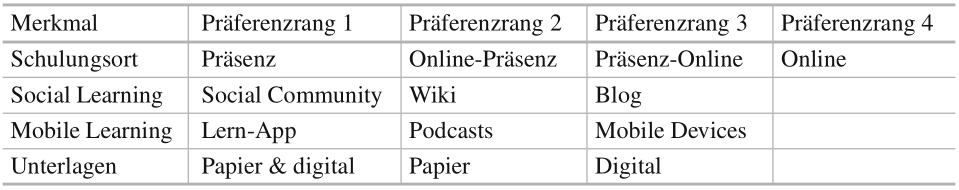
\includegraphics[width=0.8\linewidth]{./images/Marketingcontrolling/Rangfolge} \end{center}

\end{frame}

\begin{frame}{Relevanz der Merkmale}
\protect\hypertarget{relevanz-der-merkmale}{}

\textbf{Relevanz} =
\(\frac{ Spannweite (coef) }{ sum Spannweite (coef) }\)

\begin{itemize}
\item
  Das Merkmal mit der höchsten Spannweite hat folglich den
  \textbf{größten Effekt} auf die Auswahlwahrscheinlichkeit eines
  Seminarangebotes.
\item
  Änderungen bei dem Merkmal mit dem größten Effekt wirken sich auch am
  stärksten auf das Verhalten der Kunden aus, da eine \textbf{Variation
  der Ausprägung} dieses Merkmals einen bedeutsamen Einfluss auf die
  Höhe des Gesamtnutzenwertes hat
\end{itemize}

\end{frame}

\begin{frame}{Relative Wichtigkeit der Merkmale}
\protect\hypertarget{relative-wichtigkeit-der-merkmale}{}

\begin{center}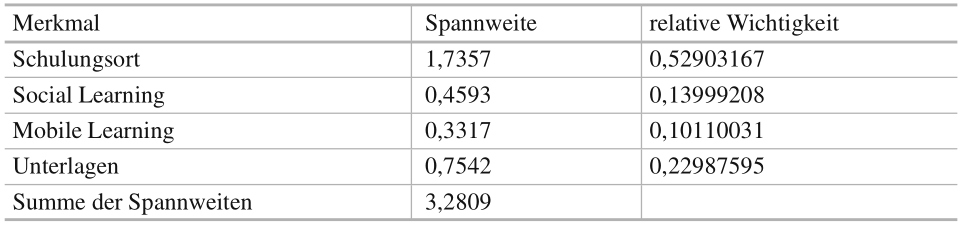
\includegraphics[width=0.8\linewidth]{./images/Marketingcontrolling/Wichtigkeit} \end{center}

\end{frame}

\begin{frame}{Übung 19: Reihenfolge der Präferenzen}
\protect\hypertarget{ubung-19-reihenfolge-der-praferenzen}{}

Für welche Präferenzreihenfolge würden Sie sich entscheiden?

\begin{enumerate}
[A.]
\tightlist
\item
  Ort:Online-Präsenz, SL: Wiki, ML: Podcast, Unt: Digital
\item
  Ort:Präsenz, SL: Social Community, ML: Lern-App, Unt: Papier \&
  Digital
\item
  Ort:online, Rest egal
\item
  Ort:ONline, SL: Wiki, ML: Podcast, Unt: Papier \& Digital
\end{enumerate}

\note{\textbf{\emph{B}}}

\end{frame}

\hypertarget{dimensionsreduktion-bei-marketingdaten}{%
\section{Dimensionsreduktion bei
Marketingdaten}\label{dimensionsreduktion-bei-marketingdaten}}

\begin{frame}{Lerziele}
\protect\hypertarget{lerziele}{}

\begin{itemize}
\tightlist
\item
  Einsatz und Ziel der Dimensionsreduktion verstehen.
\item
  Daten für die Dimensionsreduktion aufbereiten.
\item
  Anwendung der Dimensionsreduktion.
\item
  Interpretation und Schlussfolgerungen der Dimensionsreduktion.
\item
  Evaluation des Einsates der Dimensionsreduktion in der Marketing
  Controlling Praxis.
\end{itemize}

\end{frame}

\begin{frame}{Dimensionsreduktion}
\protect\hypertarget{dimensionsreduktion}{}

Datensätze im Marketing, haben oft viele Variablen - oder auch
Dimensionen - und es ist vorteilhaft, diese auf eine kleinere Anzahl von
Variablen zu \textbf{reduzieren}.

Ziel:

\textbf{Zusammenhänge} zwischen verschiedenen Dimensionen oder
\textbf{Unterschiede} zwischen verschiedenen Gruppen bezüglich einer
oder mehrerer Dimensionen (z.\thinspace{}B. bei Experimenten) können so
\textbf{klarer und einfacher identifiziert} werden.

\end{frame}

\begin{frame}[fragile]{Zwei Methoden der Dimensionsreduktion}
\protect\hypertarget{zwei-methoden-der-dimensionsreduktion}{}

\begin{itemize}
\tightlist
\item
  Die \emph{Hauptkomponentenanalyse (PCA)} versucht, unkorrelierte
  Linearkombinationen zu finden, die die maximale Varianz in den Daten
  erfassen. Die PCA beinhaltet also das Extrahieren von linearen
  Zusammenhängen der beobachteten Variablen.
\item
  Die \emph{Exploratorische Faktorenanalyse (EFA)} versucht, die Varianz
  auf Basis einer kleinen Anzahl von Dimensionen zu modellieren, während
  sie gleichzeitig versucht, die Dimensionen in Bezug auf die
  ursprünglichen Variablen interpretierbar zu machen. Es wird davon
  ausgegangen, dass die Daten einem Faktoren Modell entsprechen, bei der
  die beobachteten Korrelationen auf \texttt{latente} Faktoren
  zurückführen. Mit der EFA wird nicht die gesamte Varianz erklärt.
\end{itemize}

\end{frame}

\begin{frame}[fragile]{Welches ist die bessere Methode?}
\protect\hypertarget{welches-ist-die-bessere-methode}{}

Beide Methoden ergeben in der Regel ähnliche inhaltliche
Schlussfolgerungen.

Dies erklärt, warum einige Statistik-Software-Programme beide Methoden
zusammenpacken. So wird die PCA als Standard-Extraktionsmethode in den
SPSS-Faktoranalyse-Routinen verwendet. Dies führt zweifellos zu einer
gewissen Verwirrung über die Unterscheidung zwischen den beiden
Methoden. Die EFA wird oft als
\texttt{Common\ Factor\ Analysis\ oder\ principal\ axis\ factoring\ (Hauptachsenanalyse)}
bezeichnet. EFA verwendet eine Vielzahl von Optimierungsroutinen und das
Ergebnis, im Gegensatz zu PCA, hängt von der verwendeten
Optimierungsroutine und Ausgangspunkten für diese Routinen ab.

Es gibt also keine einzigartige Lösung bei der EFA.

\end{frame}

\begin{frame}{Faustregeln}
\protect\hypertarget{faustregeln}{}

Eine einfache Faustregel für die Entscheidung zwischen diesen beiden
Methoden:

\begin{itemize}
\tightlist
\item
  Führe die PCA durch, wenn die korrelierten beobachteten Variablen
  einfach auf einen kleineren Satz von wichtigen unabhängigen
  zusammengesetzten Variablen reduziert werden soll.
\item
  Führe die EFA durch, wenn ein theoretisches Modell von latenten
  Faktoren zugrunde liegt, dass die beobachtete Variablen verursacht.
\end{itemize}

\end{frame}

\begin{frame}{Übung 20: Methodenauswahl}
\protect\hypertarget{ubung-20-methodenauswahl}{}

welche Methode wählen Sie aus, wenn Sie in einer Ansammlung von 50 KPIs
verdichten wollen?

\begin{enumerate}
[A.]
\tightlist
\item
  PCA
\item
  EFA
\item
  KPIs lassen sich nicht verdichten
\end{enumerate}

\note{\textbf{\emph{A}}}

\end{frame}

\begin{frame}{Daten zur Markenbewertung}
\protect\hypertarget{daten-zur-markenbewertung}{}

Wir untersuchen die Dimensionalität anhand eines simulierten
Datensatzes, der typisch für \textbf{Markenwahrnehmungsstudien} ist.

Diese Daten spiegeln die Verbraucherbewertungen von Marken in Bezug auf
Wahrnehmungsadjektive wider, wie sie in der folgenden Form auf
Befragungsobjekten ausgedrückt werden:

Quelle: Chapman, C; McDonnell Feit, E. (2014): R for Marketing Research
and Analytics, Springer. (Kapitel 8)

\end{frame}

\begin{frame}[fragile]{Benötigte Pakete}
\protect\hypertarget{benotigte-pakete}{}

Pakete, die für diese Datenanalyse benötigt werden, müssen vorher
einmalig in R installiert werden.

\begin{Shaded}
\begin{Highlighting}[]
\CommentTok{# install.packages("corrplot")}
\CommentTok{# install.packages("gplots")}
\CommentTok{# install.packages("nFactors")}
\CommentTok{# install.packages("gplots")}
\CommentTok{# install.packages("RColorBrewer")}
\end{Highlighting}
\end{Shaded}

\end{frame}

\begin{frame}{Daten}
\protect\hypertarget{daten}{}

Auf einer Skala von 1 bis 10 - wobei 1 am wenigsten und 10 am meisten
ist - ist {[}brand{]} ist {[}adjektiv{]}?

In diesen Daten ist eine Beobachtung die Bewertung einer Marke durch
einen Befragten auf einem der Adjektive.

Beispiel:

\begin{enumerate}
\tightlist
\item
  Wie trendy ist FOM?
\item
  Wie hoch schätzen Sie die FOM als Marktführer ein?
\end{enumerate}

Die Daten umfassen simulierte Bewertungen von 10 Marken (``a'' bis
``j'') zu 9 Adjektiven.

\end{frame}

\begin{frame}[fragile,shrink]{Einlesen}
\protect\hypertarget{einlesen}{}

Download und Einlesen der Daten mit dem Befehl read.csv.Wir schauen uns
auch gleich den Datensatz mit head() an.

\begin{Shaded}
\begin{Highlighting}[]
\NormalTok{brand.ratings <-}\StringTok{ }\KeywordTok{read.csv}\NormalTok{(}\StringTok{"http://goo.gl/IQl8nc"}\NormalTok{)}

\KeywordTok{head}\NormalTok{(brand.ratings)}
\end{Highlighting}
\end{Shaded}

\begin{verbatim}
##   perform leader latest fun serious bargain value trendy rebuy brand
## 1       2      4      8   8       2       9     7      4     6     a
## 2       1      1      4   7       1       1     1      2     2     a
## 3       2      3      5   9       2       9     5      1     6     a
## 4       1      6     10   8       3       4     5      2     1     a
## 5       1      1      5   8       1       9     9      1     1     a
## 6       2      8      9   5       3       8     7      1     2     a
\end{verbatim}

\end{frame}

\begin{frame}[fragile,shrink]{Wir inspizieren die Daten des Datensatzes}
\protect\hypertarget{wir-inspizieren-die-daten-des-datensatzes}{}

\begin{Shaded}
\begin{Highlighting}[]
\KeywordTok{library}\NormalTok{(mosaic)}
\KeywordTok{summary}\NormalTok{(brand.ratings)}
\end{Highlighting}
\end{Shaded}

\begin{verbatim}
##     perform           leader           latest            fun        
##  Min.   : 1.000   Min.   : 1.000   Min.   : 1.000   Min.   : 1.000  
##  1st Qu.: 1.000   1st Qu.: 2.000   1st Qu.: 4.000   1st Qu.: 4.000  
##  Median : 4.000   Median : 4.000   Median : 7.000   Median : 6.000  
##  Mean   : 4.488   Mean   : 4.417   Mean   : 6.195   Mean   : 6.068  
##  3rd Qu.: 7.000   3rd Qu.: 6.000   3rd Qu.: 9.000   3rd Qu.: 8.000  
##  Max.   :10.000   Max.   :10.000   Max.   :10.000   Max.   :10.000  
##                                                                     
##     serious          bargain           value            trendy     
##  Min.   : 1.000   Min.   : 1.000   Min.   : 1.000   Min.   : 1.00  
##  1st Qu.: 2.000   1st Qu.: 2.000   1st Qu.: 2.000   1st Qu.: 3.00  
##  Median : 4.000   Median : 4.000   Median : 4.000   Median : 5.00  
##  Mean   : 4.323   Mean   : 4.259   Mean   : 4.337   Mean   : 5.22  
##  3rd Qu.: 6.000   3rd Qu.: 6.000   3rd Qu.: 6.000   3rd Qu.: 7.00  
##  Max.   :10.000   Max.   :10.000   Max.   :10.000   Max.   :10.00  
##                                                                    
##      rebuy            brand    
##  Min.   : 1.000   a      :100  
##  1st Qu.: 1.000   b      :100  
##  Median : 3.000   c      :100  
##  Mean   : 3.727   d      :100  
##  3rd Qu.: 5.000   e      :100  
##  Max.   :10.000   f      :100  
##                   (Other):400
\end{verbatim}

\end{frame}

\begin{frame}[fragile,shrink]{Neuskalierung der Daten}
\protect\hypertarget{neuskalierung-der-daten}{}

In vielen Fällen ist es sinnvoll, Rohdaten neu zu skalieren. Dies wird
üblicherweise als \textbf{Standardisierung}, \textbf{Normierung}, oder
\textbf{Z Scoring/Transformation} bezeichnet. Als Ergebnis ist der
Mittelwert aller Variablen über alle Beobachtungen dann 0. Da wir hier
gleiche Skalenstufen haben, ist ein Skalieren nicht unbedingt notwendig,
wir führen es aber trotzdem durch.

Ein einfacher Weg, alle Variablen im Datensatz auf einmal zu skalieren
ist der Befehl \texttt{scale()}. Da wir die Rohdaten nie ändern wollen,
weisen wir die Rohwerte zuerst einem neuen Dataframe \texttt{Werte.sc}
zu und skalieren anschließend die Daten. Wir skalieren in unserem
Datensatz alle Variablen.

\begin{Shaded}
\begin{Highlighting}[]
\NormalTok{brand.sc <-}\StringTok{ }\NormalTok{brand.ratings}
\NormalTok{brand.sc[, }\DecValTok{1}\OperatorTok{:}\DecValTok{9}\NormalTok{] <-}\StringTok{ }\KeywordTok{scale}\NormalTok{(brand.ratings[, }\DecValTok{1}\OperatorTok{:}\DecValTok{9}\NormalTok{])}
\KeywordTok{summary}\NormalTok{(brand.sc)}
\end{Highlighting}
\end{Shaded}

\begin{verbatim}
##     perform            leader            latest       
##  Min.   :-1.0888   Min.   :-1.3100   Min.   :-1.6878  
##  1st Qu.:-1.0888   1st Qu.:-0.9266   1st Qu.:-0.7131  
##  Median :-0.1523   Median :-0.1599   Median : 0.2615  
##  Mean   : 0.0000   Mean   : 0.0000   Mean   : 0.0000  
##  3rd Qu.: 0.7842   3rd Qu.: 0.6069   3rd Qu.: 0.9113  
##  Max.   : 1.7206   Max.   : 2.1404   Max.   : 1.2362  
##                                                       
##       fun              serious           bargain        
##  Min.   :-1.84677   Min.   :-1.1961   Min.   :-1.22196  
##  1st Qu.:-0.75358   1st Qu.:-0.8362   1st Qu.:-0.84701  
##  Median :-0.02478   Median :-0.1163   Median :-0.09711  
##  Mean   : 0.00000   Mean   : 0.0000   Mean   : 0.00000  
##  3rd Qu.: 0.70402   3rd Qu.: 0.6036   3rd Qu.: 0.65279  
##  Max.   : 1.43281   Max.   : 2.0434   Max.   : 2.15258  
##                                                         
##      value             trendy             rebuy             brand    
##  Min.   :-1.3912   Min.   :-1.53897   Min.   :-1.0717   a      :100  
##  1st Qu.:-0.9743   1st Qu.:-0.80960   1st Qu.:-1.0717   b      :100  
##  Median :-0.1405   Median :-0.08023   Median :-0.2857   c      :100  
##  Mean   : 0.0000   Mean   : 0.00000   Mean   : 0.0000   d      :100  
##  3rd Qu.: 0.6933   3rd Qu.: 0.64914   3rd Qu.: 0.5003   e      :100  
##  Max.   : 2.3610   Max.   : 1.74319   Max.   : 2.4652   f      :100  
##                                                         (Other):400
\end{verbatim}

Die Daten wurden richtig skaliert, da der Mittelwert aller Variablen
über alle Beobachtungen 0 ist.

\end{frame}

\begin{frame}[fragile,shrink]{Zusammenhänge in den Daten}
\protect\hypertarget{zusammenhange-in-den-daten}{}

Wir verwenden den Befehl \texttt{corrplot()} für die Erstinspektion von
bivariaten Beziehungen zwischen den Variablen. Das Argument
\texttt{order\ =\ "hclust"} ordnet die Zeilen und Spalten entsprechend
der Ähnlichkeit der Variablen in einer hierarchischen Cluster-Lösung der
Variablen (mehr dazu im Teil \emph{Clusteranalyse}) neu an.

\begin{Shaded}
\begin{Highlighting}[]
\KeywordTok{library}\NormalTok{(corrplot)}
\KeywordTok{corrplot}\NormalTok{(}\KeywordTok{cor}\NormalTok{(brand.sc[, }\DecValTok{1}\OperatorTok{:}\DecValTok{9}\NormalTok{]), }\DataTypeTok{order=}\StringTok{"hclust"}\NormalTok{)}
\end{Highlighting}
\end{Shaded}

\begin{center}\includegraphics{Marketing-Controlling_files/figure-beamer/unnamed-chunk-58-1} \end{center}

\end{frame}

\begin{frame}{Übung 21: Korrelationen}
\protect\hypertarget{ubung-21-korrelationen}{}

Wie viele Cluster sind sichbar?

\begin{enumerate}
[A.]
\tightlist
\item
  2
\item
  3
\item
  4
\item
  5
\end{enumerate}

\note{\textbf{\emph{B}}}

\end{frame}

\begin{frame}{Übung 22: Cluster}
\protect\hypertarget{ubung-22-cluster}{}

Welche Adjektive lassen sich aufgrund der Korrelationen zu CLustern
zusammenfassen?

\note{\begin{itemize}
\tightlist
\item
  fun/latest/trendy
\item
  rebuy/bargain/value
\item
  perform/leader/serious
\end{itemize}}

\end{frame}

\begin{frame}[fragile,shrink]{Aggregierte Durchschnittswerte nach Marke}
\protect\hypertarget{aggregierte-durchschnittswerte-nach-marke}{}

Wie berechnet man den Durchschnitt (mittlere) Position der einzelnen
Marken auf jedem Adjektiv?"

\begin{Shaded}
\begin{Highlighting}[]
\NormalTok{brand.mean <-}\StringTok{ }\KeywordTok{aggregate}\NormalTok{(. }\OperatorTok{~}\StringTok{ }\NormalTok{brand, }\DataTypeTok{data=}\NormalTok{brand.sc, mean)}
\KeywordTok{rownames}\NormalTok{(brand.mean) <-}\StringTok{ }\NormalTok{brand.mean[, }\DecValTok{1}\NormalTok{] }\CommentTok{# Marke für die Zeilennamen verwenden}
\NormalTok{brand.mean <-}\StringTok{ }\NormalTok{brand.mean[, }\DecValTok{-1}\NormalTok{]          }\CommentTok{# Markenspalte entfernen}
\NormalTok{brand.mean}
\end{Highlighting}
\end{Shaded}

\begin{verbatim}
##       perform     leader     latest        fun     serious     bargain
## a -0.88591874 -0.5279035  0.4109732  0.6566458 -0.91894067  0.21409609
## b  0.93087022  1.0707584  0.7261069 -0.9722147  1.18314061  0.04161938
## c  0.64992347  1.1627677 -0.1023372 -0.8446753  1.22273461 -0.60704302
## d -0.67989112 -0.5930767  0.3524948  0.1865719 -0.69217505 -0.88075605
## e -0.56439079  0.1928362  0.4564564  0.2958914  0.04211361  0.55155051
## f -0.05868665  0.2695106 -1.2621589 -0.2179102  0.58923066  0.87400696
## g  0.91838369 -0.1675336 -1.2849005 -0.5167168 -0.53379906  0.89650392
## h -0.01498383 -0.2978802  0.5019396  0.7149495 -0.14145855 -0.73827529
## i  0.33463879 -0.3208825  0.3557436  0.4124989 -0.14865746 -0.25459062
## j -0.62994504 -0.7885965 -0.1543180  0.2849595 -0.60218870 -0.09711188
##         value      trendy       rebuy
## a  0.18469264 -0.52514473 -0.59616642
## b  0.15133957  0.74030819  0.23697320
## c -0.44067747  0.02552787 -0.13243776
## d -0.93263529  0.73666135 -0.49398892
## e  0.41816415  0.13857986  0.03654811
## f  1.02268859 -0.81324496  1.35699580
## g  1.25616009 -1.27639344  1.36092571
## h -0.78254646  0.86430070 -0.60402622
## i -0.80339213  0.59078782 -0.20317603
## j -0.07379367 -0.48138267 -0.96164748
\end{verbatim}

\end{frame}

\begin{frame}[fragile,shrink]{Visualisierung der Rohdaten}
\protect\hypertarget{visualisierung-der-rohdaten}{}

\textbf{Heatmap der Attribute nach Marke}

\begin{Shaded}
\begin{Highlighting}[]
\KeywordTok{library}\NormalTok{(gplots)}
\KeywordTok{library}\NormalTok{(RColorBrewer)}
\KeywordTok{heatmap.2}\NormalTok{(}\KeywordTok{as.matrix}\NormalTok{(brand.mean),}
         \DataTypeTok{col=}\KeywordTok{brewer.pal}\NormalTok{(}\DecValTok{9}\NormalTok{, }\StringTok{"Blues"}\NormalTok{), }\DataTypeTok{trace=}\StringTok{"none"}\NormalTok{, }\DataTypeTok{key=}\OtherTok{FALSE}\NormalTok{, }\DataTypeTok{dend=}\StringTok{"none"}\NormalTok{,}
         \DataTypeTok{main=}\StringTok{"Markenbewertung"}\NormalTok{)}
\end{Highlighting}
\end{Shaded}

\begin{center}\includegraphics{Marketing-Controlling_files/figure-beamer/unnamed-chunk-60-1} \end{center}

\end{frame}

\begin{frame}[fragile,shrink]{Wahrnehmungsraum der Marken}
\protect\hypertarget{wahrnehmungsraum-der-marken}{}

\begin{Shaded}
\begin{Highlighting}[]
\NormalTok{brand.mu.pc <-}\StringTok{ }\KeywordTok{prcomp}\NormalTok{(brand.mean, }\DataTypeTok{scale=}\OtherTok{TRUE}\NormalTok{)}
\KeywordTok{biplot}\NormalTok{(brand.mu.pc, }\DataTypeTok{main=}\StringTok{"Wahrnehmungsraum"}\NormalTok{)}
\end{Highlighting}
\end{Shaded}

\begin{center}\includegraphics{Marketing-Controlling_files/figure-beamer/unnamed-chunk-61-1} \end{center}

\end{frame}

\begin{frame}{Hauptkomponentenanalyse (PCA)}
\protect\hypertarget{hauptkomponentenanalyse-pca}{}

Die PCA berechnet ein Variablenset (Komponenten) in Form von linearen
Gleichungen, die die linearen Beziehungen in den Daten erfassen.

Die erste Komponente erfasst so viel Streuung (Varianz) wie möglich von
allen Variablen als eine einzige lineare Funktion.

Die zweite Komponente erfasst unkorreliert zur ersten Komponente so viel
Streuung wie möglich, die nach der ersten Komponente verbleibt.

Das geht so lange weiter, bis es so viele Komponenten gibt wie
Variablen.

\end{frame}

\begin{frame}[fragile]{Scree-Plot}
\protect\hypertarget{scree-plot}{}

Der Standard-Plot \texttt{plot()} für die PCA ist ein
\textbf{Scree-Plot}, dieser zeigt uns in Reihenfolge der
Hauptkomponenten jeweils die durch diese Hauptkomponente erfasste
Streuung (Varianz).

\begin{itemize}
\tightlist
\item
  Es soll die Stelle gefunden werden, ab der die Varianzen der
  Hauptkomponenten deutlich kleiner sind.
\item
  Je kleiner die Varianzen, desto weniger Streuung erklärt diese
  Hauptkomponente.
\end{itemize}

\end{frame}

\begin{frame}{Elbow-Kriterium}
\protect\hypertarget{elbow-kriterium}{}

Nach diesem Kriterium werden alle Hauptkomponenten berücksichtigt, die
links von der Knickstelle im Scree-Plot liegen.

Gibt es mehrere Knicks, dann werden jene Hauptkomponenten ausgewählt,
die links vom rechtesten Knick liegen.

Gibt es keinen Knick, dann hilft der Scree-Plot nicht weiter.

\end{frame}

\begin{frame}[fragile,shrink]{Eigenwert-Kriterium}
\protect\hypertarget{eigenwert-kriterium}{}

Der Eigenwert ist eine Metrik für den Anteil der erklärten Varianz. Die
Anzahl Eigenwerte können wir über den Befehl \texttt{eigen()} ausgeben.
An dieser Stelle können wir die original Daten nehmen, da wir keine
unterschiedlichen Skalenstufen haben. Der Eigenwert einer
Komponente\thinspace{}/\thinspace{}eines Faktors sagt aus, wie viel
Varianz dieser Faktor an der Gesamtvarianz aufklärt. Laut dem
Eigenwert-Kriterium sollen nur Faktoren mit einem Eigenwert größer 1
extrahiert werden

\begin{Shaded}
\begin{Highlighting}[]
\KeywordTok{eigen}\NormalTok{(}\KeywordTok{cor}\NormalTok{(brand.sc[, }\DecValTok{1}\OperatorTok{:}\DecValTok{9}\NormalTok{]))}
\end{Highlighting}
\end{Shaded}

\begin{verbatim}
## eigen() decomposition
## $values
## [1] 2.9792956 2.0965517 1.0792549 0.7272110 0.6375459 0.5348432 0.3901044
## [8] 0.3120464 0.2431469
## 
## $vectors
##             [,1]        [,2]        [,3]        [,4]        [,5]
##  [1,] -0.2374679 -0.41991179  0.03854006  0.52630873  0.46793435
##  [2,] -0.2058257 -0.52381901 -0.09512739  0.08923461 -0.29452974
##  [3,]  0.3703806 -0.20145317 -0.53273054 -0.21410754  0.10586676
##  [4,]  0.2510601  0.25037973 -0.41781346  0.75063952 -0.33149429
##  [5,] -0.1597402 -0.51047254 -0.04067075 -0.09893394 -0.55515540
##  [6,] -0.3991731  0.21849698 -0.48989756 -0.16734345 -0.01257429
##  [7,] -0.4474562  0.18980822 -0.36924507 -0.15118500 -0.06327757
##  [8,]  0.3510292 -0.31849032 -0.37090530 -0.16764432  0.36649697
##  [9,] -0.4390184 -0.01509832 -0.12461593  0.13031231  0.35568769
##             [,6]         [,7]        [,8]        [,9]
##  [1,]  0.3370676  0.364179109 -0.14444718 -0.05223384
##  [2,]  0.2968860 -0.613674301  0.28766118  0.17889453
##  [3,]  0.1742059 -0.185480310 -0.64290436 -0.05750244
##  [4,] -0.1405367 -0.007114761  0.07461259 -0.03153306
##  [5,] -0.3924874  0.445302862 -0.18354764 -0.09072231
##  [6,]  0.1393966  0.288264900  0.05789194  0.64720849
##  [7,]  0.2195327  0.017163011  0.14829295 -0.72806108
##  [8,] -0.2658186  0.153572108  0.61450289 -0.05907022
##  [9,] -0.6751400 -0.388656160 -0.20210688  0.01720236
\end{verbatim}

\end{frame}

\begin{frame}[fragile,shrink]{Scree-Plot}
\protect\hypertarget{scree-plot-1}{}

Dies kann auch grafisch mit dem \texttt{VSS.Scree} geplotet werden.

\begin{Shaded}
\begin{Highlighting}[]
\KeywordTok{library}\NormalTok{(nFactors)}
\KeywordTok{VSS.scree}\NormalTok{(brand.sc[, }\DecValTok{1}\OperatorTok{:}\DecValTok{9}\NormalTok{])}
\end{Highlighting}
\end{Shaded}

\begin{center}\includegraphics{Marketing-Controlling_files/figure-beamer/unnamed-chunk-63-1} \end{center}

\end{frame}

\begin{frame}{Übung 23: Anzahl Hauptkomponenten}
\protect\hypertarget{ubung-23-anzahl-hauptkomponenten}{}

Wie viele Hauptkomponenten lasse sich extrahieren?

\begin{enumerate}
[A.]
\tightlist
\item
  1
\item
  2
\item
  3
\item
  4
\end{enumerate}

\note{\textbf{\emph{C}}}

\end{frame}

\begin{frame}[fragile,shrink]{Extraktion der Komponenten}
\protect\hypertarget{extraktion-der-komponenten}{}

Am einfachsten lassen sich die Komponenten extrahieren mit dem
\texttt{principal}-Befehl aus dem psych-Paket (ist durch das Paket
nFactors bereits geladen)

\begin{Shaded}
\begin{Highlighting}[]
\NormalTok{brands.pca<-}\KeywordTok{principal}\NormalTok{(brand.sc[, }\DecValTok{1}\OperatorTok{:}\DecValTok{9}\NormalTok{], }\DataTypeTok{nfactors=}\DecValTok{3}\NormalTok{)}
\KeywordTok{print}\NormalTok{(brands.pca, }\DataTypeTok{cut=}\FloatTok{0.5}\NormalTok{, }\DataTypeTok{sort =} \OtherTok{TRUE}\NormalTok{, }\DataTypeTok{digits=}\DecValTok{2}\NormalTok{)}
\end{Highlighting}
\end{Shaded}

\begin{verbatim}
## Principal Components Analysis
## Call: principal(r = brand.sc[, 1:9], nfactors = 3)
## Standardized loadings (pattern matrix) based upon correlation matrix
##         item   RC2   RC1   RC3   h2   u2 com
## leader     2  0.83             0.71 0.29 1.1
## serious    5  0.78             0.62 0.38 1.0
## perform    1  0.72             0.54 0.46 1.1
## fun        4 -0.53             0.51 0.49 2.0
## bargain    6        0.91       0.83 0.17 1.0
## value      7        0.88       0.82 0.18 1.1
## rebuy      9        0.62       0.59 0.41 2.0
## latest     3              0.87 0.80 0.20 1.1
## trendy     8              0.77 0.73 0.27 1.5
## 
##                        RC2  RC1  RC3
## SS loadings           2.24 2.16 1.76
## Proportion Var        0.25 0.24 0.20
## Cumulative Var        0.25 0.49 0.68
## Proportion Explained  0.36 0.35 0.29
## Cumulative Proportion 0.36 0.71 1.00
## 
## Mean item complexity =  1.3
## Test of the hypothesis that 3 components are sufficient.
## 
## The root mean square of the residuals (RMSR) is  0.08 
##  with the empirical chi square  509.66  with prob <  1.9e-101 
## 
## Fit based upon off diagonal values = 0.93
\end{verbatim}

\end{frame}

\begin{frame}[fragile]{Übung 24: Interpretation der PCA Ergebnisse}
\protect\hypertarget{ubung-24-interpretation-der-pca-ergebnisse}{}

Wie interpretieren Sie das Ergebnis? Diskutieren Sie mögliche Lösungen.

\note{\begin{itemize}
\tightlist
\item
  Das Ergebnis sieht sehr gut aus. Es laden immer mehrere Items
  (mindestens 2) hoch (\textgreater{} 0,5) auf einer Komponente (die mit
  RC1 bis RC3 bezeichnet werden, RC steht für Rotated Component).
  Innerhalb einer PCA kann die Interpretierbarkeit über eine
  \textbf{Rotation} erhöht werden. Wenn die Rotation nicht
  ausgeschlossen wird (mit dem Argument \texttt{rotate="none"}), dann
  ist die Voreinstellung eine \texttt{Varimax-Rotation}.\\
\item
  Es gibt keine Items die auf mehr als einer Komponente hoch laden. Die
  Ladungen sind Korrelationskoeffizienten zwischen den Items und den
  Hauptkomponenten.
\item
  In der Zeile SS loadings finden wir die Eigenwerte der fünf
  Hauptkomponenten. Den Anteil an der Gesamtvarianz, den sie erklären,
  findet man in der Zeile Proportion Var. Aufsummiert sind die Anteile
  in der Zeile Cumlative Var. Insgesamt werden durch die fünf
  Hauptkomponenten \mbox{64\thinspace{}\%}\xspace{} der Gesamtvarianz
  erklärt.
\item
  Einzig das Item \texttt{fun} lädt negativ auf RC2.
\end{itemize}}

\end{frame}

\begin{frame}{Exploratorische Faktorenanalyse (EFA)}
\protect\hypertarget{exploratorische-faktorenanalyse-efa}{}

EFA ist eine Methode, um die Beziehung von Konstrukten (Konzepten),
d.\thinspace{}h. Faktoren zu Variablen zu beurteilen. Dabei werden die
Faktoren als \textbf{latente Variablen} betrachtet, die nicht direkt
beobachtet werden können.

Stattdessen werden sie empirisch durch mehrere Variablen beobachtet, von
denen jede ein Indikator der zugrundeliegenden Faktoren ist. Diese
beobachteten Werte werden als \textbf{manifeste Variablen} bezeichnet
und umfassen Indikatoren.

Die EFA versucht den Grad zu bestimmen, in dem Faktoren die beobachtete
Streuung der manifesten Variablen berücksichtigen.

\end{frame}

\begin{frame}{Vergleich zur PCA}
\protect\hypertarget{vergleich-zur-pca}{}

Das Ergebnis der EFA ist ähnlich zur PCA: eine Matrix von Faktoren
(ähnlich zu den PCA-Komponenten) und ihre Beziehung zu den
ursprünglichen Variablen (Ladung der Faktoren auf die Variablen).

Im Gegensatz zur PCA versucht die EFA, Lösungen zu finden, die in den
\textbf{manifesten Variablen maximal interpretierbar} sind.

Im Allgemeinen versucht sie, Lösungen zu finden, bei denen eine kleine
Anzahl von Ladungen für jeden Faktor sehr hoch ist, während andere
Ladungen für diesen Faktor gering sind. Wenn dies möglich ist, kann
dieser Faktor mit diesem Variablen-Set interpretiert werden.

\end{frame}

\begin{frame}[fragile]{Finden einer EFA Lösung}
\protect\hypertarget{finden-einer-efa-losung}{}

Als erstes muss die Anzahl der zu schätzenden Faktoren bestimmt werden.
Hierzu verwenden wir wieder das Ellbow-Kriterium und das
Eigenwert-Kriterium. Beide Kriterien haben wir schon bei der PCA
verwendet, dabei kommen wir auf 3 Faktoren.

Durch das Paket \texttt{nFactors} bekommen wir eine formalisierte
Berechnung der Scree-Plot Lösung mit dem Befehl \texttt{nScree()}

\begin{Shaded}
\begin{Highlighting}[]
\KeywordTok{library}\NormalTok{(nFactors)}
\KeywordTok{nScree}\NormalTok{(brand.sc[, }\DecValTok{1}\OperatorTok{:}\DecValTok{9}\NormalTok{])}
\end{Highlighting}
\end{Shaded}

\begin{verbatim}
##   noc naf nparallel nkaiser
## 1   3   2         3       3
\end{verbatim}

\texttt{nScree} gibt vier methodische Schätzungen für die Anzahl an
Faktoren durch den Scree-Plot aus. Wir sehen, dass drei von vier
Methoden 3 Faktoren vorschlagen.

\end{frame}

\begin{frame}[fragile,shrink]{Schätzung der EFA}
\protect\hypertarget{schatzung-der-efa}{}

Eine EFA wird geschätzt mit dem Befehl \texttt{factanal(x,factors=k)},
wobei \texttt{k} die Anzahl Faktoren angibt.

\begin{Shaded}
\begin{Highlighting}[]
\NormalTok{brands.fa<-}\KeywordTok{factanal}\NormalTok{(brand.sc[, }\DecValTok{1}\OperatorTok{:}\DecValTok{9}\NormalTok{], }\DataTypeTok{factors=}\DecValTok{3}\NormalTok{)}
\NormalTok{brands.fa}
\end{Highlighting}
\end{Shaded}

\begin{verbatim}
## 
## Call:
## factanal(x = brand.sc[, 1:9], factors = 3)
## 
## Uniquenesses:
## perform  leader  latest     fun serious bargain   value  trendy   rebuy 
##   0.624   0.327   0.005   0.794   0.530   0.302   0.202   0.524   0.575 
## 
## Loadings:
##         Factor1 Factor2 Factor3
## perform          0.607         
## leader           0.810   0.106 
## latest  -0.163           0.981 
## fun             -0.398   0.205 
## serious          0.682         
## bargain  0.826          -0.122 
## value    0.867          -0.198 
## trendy  -0.356           0.586 
## rebuy    0.499   0.296  -0.298 
## 
##                Factor1 Factor2 Factor3
## SS loadings      1.853   1.752   1.510
## Proportion Var   0.206   0.195   0.168
## Cumulative Var   0.206   0.401   0.568
## 
## Test of the hypothesis that 3 factors are sufficient.
## The chi square statistic is 64.57 on 12 degrees of freedom.
## The p-value is 3.28e-09
\end{verbatim}

\end{frame}

\begin{frame}[fragile,shrink]{Schönere Ausgabe der EFA}
\protect\hypertarget{schonere-ausgabe-der-efa}{}

Eine übersichtlichere Ausgabe bekommen wir mit dem \texttt{print}
Befehl, in dem wir zusätzlich noch die Dezimalstellen kürzen mit
\texttt{digits=2}, alle Ladungen kleiner als 0,5 ausblenden mit
\texttt{cutoff=.4} und die Ladungen mit \texttt{sort=TRUE} so sortieren,
dass die Ladungen, die auf einen Faktor laden, untereinander stehen.

\begin{Shaded}
\begin{Highlighting}[]
\KeywordTok{print}\NormalTok{(brands.fa, }\DataTypeTok{digits=}\DecValTok{2}\NormalTok{, }\DataTypeTok{cutoff=}\NormalTok{.}\DecValTok{4}\NormalTok{, }\DataTypeTok{sort=}\OtherTok{TRUE}\NormalTok{)}
\end{Highlighting}
\end{Shaded}

\begin{verbatim}
## 
## Call:
## factanal(x = brand.sc[, 1:9], factors = 3)
## 
## Uniquenesses:
## perform  leader  latest     fun serious bargain   value  trendy   rebuy 
##    0.62    0.33    0.00    0.79    0.53    0.30    0.20    0.52    0.58 
## 
## Loadings:
##         Factor1 Factor2 Factor3
## bargain  0.83                  
## value    0.87                  
## perform          0.61          
## leader           0.81          
## serious          0.68          
## latest                   0.98  
## trendy                   0.59  
## fun                            
## rebuy    0.50                  
## 
##                Factor1 Factor2 Factor3
## SS loadings       1.85    1.75    1.51
## Proportion Var    0.21    0.19    0.17
## Cumulative Var    0.21    0.40    0.57
## 
## Test of the hypothesis that 3 factors are sufficient.
## The chi square statistic is 64.57 on 12 degrees of freedom.
## The p-value is 3.28e-09
\end{verbatim}

\end{frame}

\begin{frame}[fragile,shrink]{Heatmap mit Ladungen}
\protect\hypertarget{heatmap-mit-ladungen}{}

In der obigen Ausgabe werden die Item-to-Faktor-Ladungen angezeigt. Im
zurückgegebenen Objekt \texttt{Werte.fa} sind diese als
\texttt{\$loadings} vorhanden. Wir können die Item-Faktor-Beziehungen
mit einer Heatmap von \texttt{\$loadings} visualisieren:

\begin{Shaded}
\begin{Highlighting}[]
\KeywordTok{heatmap.2}\NormalTok{(brands.fa}\OperatorTok{$}\NormalTok{loadings,}
          \DataTypeTok{col=}\KeywordTok{brewer.pal}\NormalTok{(}\DecValTok{9}\NormalTok{, }\StringTok{"Blues"}\NormalTok{), }\DataTypeTok{trace=}\StringTok{"none"}\NormalTok{, }\DataTypeTok{key=}\OtherTok{FALSE}\NormalTok{, }\DataTypeTok{dend=}\StringTok{"none"}\NormalTok{,}
          \DataTypeTok{Colv=}\OtherTok{FALSE}\NormalTok{, }\DataTypeTok{cexCol =} \FloatTok{1.2}\NormalTok{, }\DataTypeTok{main=}\StringTok{"Ladungen brands.fa"}\NormalTok{)}
\end{Highlighting}
\end{Shaded}

\begin{center}\includegraphics{Marketing-Controlling_files/figure-beamer/unnamed-chunk-68-1} \end{center}

\end{frame}

\begin{frame}{Übung 25: Interpretation der EFA Ergebnisse}
\protect\hypertarget{ubung-25-interpretation-der-efa-ergebnisse}{}

Wie interpretieren Sie das Ergebnis?

\note{Das Ergebnis zeigt eine klare Trennung der Items in 3 Faktoren,
die grob als \textbf{Wert}, \textbf{Leader} und \textbf{Trend}
interpretierbar sind. Das item **rebuy* läd sowohl auf Faktor1 (Wert)
als auch Faktor2 (Leader). Dies deutet darauf hin, dass die Verbraucher
in den simulierten Daten sagen, sie würden eine Marke aus irgendeinem
Grund wiederkaufen, weil sie hochwertig ist oder weil sie führend ist.}

\end{frame}

\begin{frame}[fragile,shrink]{Bildung der Faktoren durch
Mittelwertbildung}
\protect\hypertarget{bildung-der-faktoren-durch-mittelwertbildung}{}

Eine Möglichkeit Faktoren zu bilden geht über die Mittelwerte der Items.
Dies ist jedoch nur sinnvoll, wenn einheitliche Skalen über alle Items
hinweg vorliegen. Wir verwenden hierfür den Befehl \texttt{rowMeans}.

\begin{Shaded}
\begin{Highlighting}[]
\NormalTok{brand.ratings}\OperatorTok{$}\NormalTok{Wert<-}\KeywordTok{rowMeans}\NormalTok{(brand.ratings[,}\KeywordTok{c}\NormalTok{(}\StringTok{"value"}\NormalTok{, }\StringTok{"bargain"}\NormalTok{, }
                                              \StringTok{"rebuy"}\NormalTok{)], }\DataTypeTok{na.rm =} \OtherTok{TRUE}\NormalTok{)}
\NormalTok{brand.ratings}\OperatorTok{$}\NormalTok{Leader<-}\KeywordTok{rowMeans}\NormalTok{(brand.ratings[,}\KeywordTok{c}\NormalTok{(}\StringTok{"serious"}\NormalTok{, }\StringTok{"perform"}\NormalTok{, }
                                                \StringTok{"leader"}\NormalTok{)], }\DataTypeTok{na.rm =} \OtherTok{TRUE}\NormalTok{)}
\NormalTok{brand.ratings}\OperatorTok{$}\NormalTok{Trend<-}\KeywordTok{rowMeans}\NormalTok{(brand.ratings[,}\KeywordTok{c}\NormalTok{(}\StringTok{"latest"}\NormalTok{, }\StringTok{"trendy"}\NormalTok{, }
                                               \StringTok{"fun"}\NormalTok{)], }\DataTypeTok{na.rm =} \OtherTok{TRUE}\NormalTok{)}
\end{Highlighting}
\end{Shaded}

\end{frame}

\begin{frame}{Interne Konsistenz der Skalen}
\protect\hypertarget{interne-konsistenz-der-skalen}{}

Das einfachste Maß für die \textbf{interne Konsistenz} ist die
\textbf{Split-Half-Reliabilität}. Die Items werden in zwei Hälften
unterteilt und die resultierenden Scores sollten in ihren Kenngrößen
ähnlich sein.

Hohe Korrelationen zwischen den Hälften deuten auf eine hohe interne
Konsistenz hin.

Das Problem ist, dass die Ergebnisse davon abhängen, wie die Items
aufgeteilt werden. Ein üblicher Ansatz zur Lösung dieses Problems
besteht darin, den Koeffizienten \textbf{Alpha (Cronbachs Alpha)} zu
verwenden.

\end{frame}

\begin{frame}{Cronbachs Alpha}
\protect\hypertarget{cronbachs-alpha}{}

Der Koeffizient \textbf{Alpha} ist der Mittelwert aller möglichen
Split-Half-Koeffizienten, die sich aus verschiedenen Arten der
Aufteilung der Items ergeben. Dieser Koeffizient variiert von 0 bis 1.
Formal ist es ein korrigierter durchschnittlicher
Korrelationskoeffizient.

Zufriedenstellende Reliabilität wird bei einem Alpha-Wert von 0.7
erreicht. Werte unter 0.5 gelten als nicht akzeptabel, Werte ab 0.8 als
gut.

\end{frame}

\begin{frame}[fragile,shrink]{Bewertung von Wert}
\protect\hypertarget{bewertung-von-wert}{}

\begin{Shaded}
\begin{Highlighting}[]
\KeywordTok{library}\NormalTok{(psych)}
\KeywordTok{alpha}\NormalTok{(brand.ratings[,}\KeywordTok{c}\NormalTok{(}\StringTok{"value"}\NormalTok{, }\StringTok{"bargain"}\NormalTok{, }\StringTok{"rebuy"}\NormalTok{)])}
\end{Highlighting}
\end{Shaded}

\begin{verbatim}
## 
## Reliability analysis   
## Call: alpha(x = brand.ratings[, c("value", "bargain", "rebuy")])
## 
##   raw_alpha std.alpha G6(smc) average_r S/N   ase mean  sd median_r
##        0.8       0.8    0.75      0.57   4 0.011  4.1 2.1     0.51
## 
##  lower alpha upper     95% confidence boundaries
## 0.78 0.8 0.82 
## 
##  Reliability if an item is dropped:
##         raw_alpha std.alpha G6(smc) average_r S/N alpha se var.r med.r
## value        0.64      0.64    0.47      0.47 1.8   0.0230    NA  0.47
## bargain      0.67      0.67    0.51      0.51 2.0   0.0207    NA  0.51
## rebuy        0.85      0.85    0.74      0.74 5.7   0.0095    NA  0.74
## 
##  Item statistics 
##            n raw.r std.r r.cor r.drop mean  sd
## value   1000  0.88  0.89  0.83   0.73  4.3 2.4
## bargain 1000  0.88  0.87  0.80   0.69  4.3 2.7
## rebuy   1000  0.78  0.78  0.57   0.52  3.7 2.5
## 
## Non missing response frequency for each item
##            1    2    3    4    5    6    7    8    9   10 miss
## value   0.15 0.11 0.15 0.14 0.13 0.12 0.09 0.07 0.03 0.02    0
## bargain 0.23 0.10 0.12 0.11 0.11 0.11 0.09 0.06 0.05 0.03    0
## rebuy   0.26 0.16 0.12 0.14 0.08 0.08 0.06 0.05 0.03 0.03    0
\end{verbatim}

\end{frame}

\begin{frame}{Übung 26: Interpretation Alpha}
\protect\hypertarget{ubung-26-interpretation-alpha}{}

Wie beurteilen Sie das Alpha von Werte?

\begin{enumerate}
[A.]
\tightlist
\item
  gut
\item
  zufriedenstellen
\item
  akzeptabel
\item
  schlecht
\end{enumerate}

\note{\textbf{\emph{A}}}

\end{frame}

\begin{frame}[fragile,shrink]{Beurteilung der Marken je Faktor}
\protect\hypertarget{beurteilung-der-marken-je-faktor}{}

\begin{Shaded}
\begin{Highlighting}[]
\NormalTok{brand.fa.mean <-}\StringTok{ }\KeywordTok{aggregate}\NormalTok{(. }\OperatorTok{~}\StringTok{ }\NormalTok{brand, }\DataTypeTok{data=}\NormalTok{brand.ratings, mean)}
\KeywordTok{rownames}\NormalTok{(brand.fa.mean) <-}\StringTok{ }\NormalTok{brand.fa.mean[, }\DecValTok{1}\NormalTok{]}
\NormalTok{brand.fa.mean <-}\StringTok{ }\NormalTok{brand.fa.mean[, }\DecValTok{-1}\NormalTok{]}
\NormalTok{brand.fa.mean <-}\StringTok{ }\NormalTok{brand.fa.mean[,}\DecValTok{10}\OperatorTok{:}\DecValTok{12}\NormalTok{]}
\KeywordTok{heatmap.2}\NormalTok{(}\KeywordTok{as.matrix}\NormalTok{(brand.fa.mean), }
          \DataTypeTok{col=}\KeywordTok{brewer.pal}\NormalTok{(}\DecValTok{9}\NormalTok{, }\StringTok{"Blues"}\NormalTok{), }\DataTypeTok{trace=}\StringTok{"none"}\NormalTok{, }\DataTypeTok{key=}\OtherTok{FALSE}\NormalTok{, }\DataTypeTok{dend=}\StringTok{"none"}\NormalTok{,}
          \DataTypeTok{cexCol=}\FloatTok{1.2}\NormalTok{, }\DataTypeTok{main=}\StringTok{"Markenbeurteilung je Faktor"}\NormalTok{)}
\end{Highlighting}
\end{Shaded}

\begin{center}\includegraphics{Marketing-Controlling_files/figure-beamer/unnamed-chunk-71-1} \end{center}

\end{frame}

\begin{frame}{Literatur}
\protect\hypertarget{literatur-1}{}

\begin{itemize}
\tightlist
\item
  Chris Chapman, Elea McDonnell Feit (2015): \emph{R for Marketing
  Research and Analytics}, Kapitel 8.1-8.3
\item
  Gareth James, Daniela Witten, Trevor Hastie, Robert Tibshirani (2013):
  \emph{An Introduction to Statistical Learning -- with Applications in
  R}, \url{http://www-bcf.usc.edu/~gareth/ISL/}, Kapitel 10.2, 10.4
\item
  Reinhold Hatzinger, Kurt Hornik, Herbert Nagel (2011): \emph{R --
  Einführung durch angewandte Statistik}. Kapitel 11
\item
  Maike Luhmann (2015): R für Einsteiger, Kapitel 19
\end{itemize}

\end{frame}

\hypertarget{mds-als-analyseverfahren}{%
\section{MDS als Analyseverfahren}\label{mds-als-analyseverfahren}}

\begin{frame}{Lernziele}
\protect\hypertarget{lernziele-5}{}

\begin{itemize}
\tightlist
\item
  Einsatz und Ziel der MDS Analyse verstehen.
\item
  Daten für die MDS aufbereiten.
\item
  Anwendung der MDS.
\item
  Interpretation und Schlussfolgerungen der MDS.
\item
  Evaluation des Einsates der MDS in der Marketing Controlling Praxis.
\end{itemize}

\end{frame}

\begin{frame}{Multidimensiononale Skalierung (MDS)}
\protect\hypertarget{multidimensiononale-skalierung-mds}{}

MDS ist eine Methode, mit der auch niedrigdimensionale Darstellungen von
Daten gefunden werden können. Statt Komponenten oder latente Faktoren
wie bei der PCA oder EFA zu extrahieren, arbeitet das MDS stattdessen
mit Entfernungen (oder Ähnlichkeiten).

Die MDS versucht, eine \textbf{niedrigdimensionale Raum} zu finden, die
alle beobachteten Ähnlichkeiten zwischen den Objekten am besten
darstellt. Die Objekte werden auf Basis ihrer \textbf{Ähnlichkeit}
zueinander dargestellt

Praktische Marketinganwendungen der MDS:

\begin{itemize}
\tightlist
\item
  Imagemessung,
\item
  Marktsegmentierung,
\item
  Entwicklung neuer Produkte,
\item
  Beurteilung der Werbewirksamkeit,
\item
  Preisanalyse,
\item
  Channel-Entscheidungen und
\item
  Erstellung von Einstellungsskalen.
\end{itemize}

\end{frame}

\begin{frame}{MDS als Verfahren zur Positionierung}
\protect\hypertarget{mds-als-verfahren-zur-positionierung}{}

Einsatz der MDS bei Positionierungsstudien:

\begin{itemize}
\tightlist
\item
  Untersuchung eines Markenraumes
\item
  Analyse der Positionierung einer bestimmten Marke
\item
  Entwicklung einer Zielvorstellung für die Neupositionierung der Marke
  im Kontext konkurrierender Marken
\item
  Überprüfung des Neupositionierungsziels nach Einsatz geeigneter
  Marketing-Instrumente
\end{itemize}

\end{frame}

\begin{frame}{Stärken der MDS}
\protect\hypertarget{starken-der-mds}{}

Konstruktion eines möglichst niedrig dimensionierten Wahrnehmungsraums
aus der ordinalen Ausgangsinformation.

Gründe für den Umweg:

\begin{itemize}
\tightlist
\item
  Verzichtet auf Vorgabe von Merkmalen um nicht auf bestimmte Merkmale
  aufmerksam zu machen.
\item
  Die Merkmale, die Personen bei Beurteilungsobjekten wahrnehmen, sind
  dem Untersuchungsleiter unbekannt.
\item
  Bei direkt erfragten Wahrnehmungen (konfirmatorischen Messungen) ist
  die interne Konsistenz der Daten nicht prüfbar
\item
  Die Merkmale sind z.\thinspace{}T. sehr subjektiver oder emotionaler
  Art, sie lassen sich nicht gut in Worte fassen.
\end{itemize}

\end{frame}

\begin{frame}{Erhebungverfahren zur Ähnlichkeit von Objekten}
\protect\hypertarget{erhebungverfahren-zur-ahnlichkeit-von-objekten}{}

\textbf{Ratingverfahren:}\\
„Beurteilen Sie paarweise die Ähnlichkeit der folgenden Automarken.
Vergeben sie für die Ähnlichkeit eines Automarkenpaares eine Zahl im
Wertebereich von 1 (= sehr ähnlich) bis 9 (= sehr unähnlich)!``

\textbf{Rangreihung:}\\
Es werden alle möglichen Paarungen von Objekten gebildet (Karteikarten)
und in eine Rangreihe gebracht (sortiert).

\textbf{Ankerpunktmethode:}\\
„Geben Sie für jedes Objekt (zeilenweise) die Reihenfolge der anderen
Objekte zu diesem Objekt an.``

\end{frame}

\begin{frame}{Auswahl der Beurteilungsobjekte}
\protect\hypertarget{auswahl-der-beurteilungsobjekte}{}

\begin{itemize}
\tightlist
\item
  Objekte müssen bekannt sein
\item
  Anzahl der Ähnlichkeiten zwischen den Objekten muss die Anzahl der
  Koordinaten im Lösungsraum deutlich übersteigen

  \begin{itemize}
  \tightlist
  \item
    Dateninput bei n Beurteilungsobjekten sind = n x (n-1)/2
    Ähnlichkeitswerte
  \item
    Datenoutput sind h x n Profilwerte (n: Anzahl der
    Beurteilungsobjekte, h: Anzahl der Dimensionen)
  \end{itemize}
\item
  Zahl der Objekte sollte nicht zu groß sein (Überforderung der Apn)
\end{itemize}

\end{frame}

\begin{frame}{Übung 27: Dateninput}
\protect\hypertarget{ubung-27-dateninput}{}

Wie viele Daten müssen für eine MDS Analyse eingegeben werden, wenn 10
Marken beurteilt werden sollen?

\begin{enumerate}
[A.]
\tightlist
\item
  50
\item
  45
\item
  10
\item
  100
\end{enumerate}

\note{\textbf{\emph{B}}}

\end{frame}

\begin{frame}{Statistische Optimierung}
\protect\hypertarget{statistische-optimierung}{}

Bei der Bestimmung der Konfiguration verwendet die MDS einen
\textbf{iterativen Prozess}.

Die \textbf{Idee} hinter diesem Prozess:

\begin{enumerate}
\tightlist
\item
  Alle Objekte werden willkürlich im Raum angeordnet.
\item
  Die Distanzen zwischen den Objekten werden nun mit den Ähnlichkeiten
  verglichen. Liegen nun zwei Objekte im Verhältnis zur Ähnlichkeit weit
  \textbf{auseinander/bei einander}, werden sie \textbf{aufeinander
  zu-/voneinander} weg geschoben
\item
  Dieser Vorgang wird so lange wiederholt, bis die Konfiguration der
  Objekte die erhobenen Ähnlichkeiten zufriedenstellend abbildet.
\end{enumerate}

\end{frame}

\begin{frame}{Statistische Optimierung}
\protect\hypertarget{statistische-optimierung-1}{}

\textbf{Minkowski-Metrik:}

\begin{center}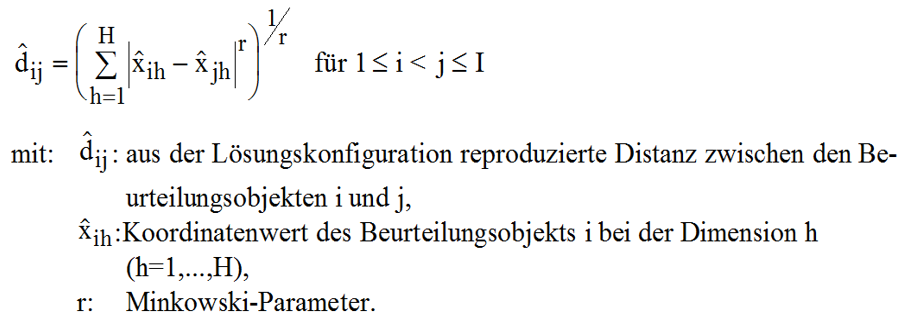
\includegraphics[width=0.7\linewidth]{./images/Marketingcontrolling/Minkowski} \end{center}

\begin{itemize}
\tightlist
\item
  Dimensionszahl H=2 und Minkowski-Parameter r=2 (euklidische Distanz)
\end{itemize}

\end{frame}

\begin{frame}{Euklidische Distanz}
\protect\hypertarget{euklidische-distanz}{}

\begin{center}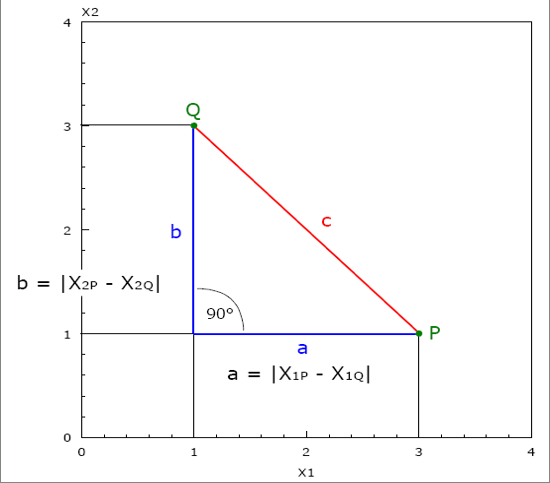
\includegraphics[width=0.5\linewidth]{./images/Marketingcontrolling/Euklid} \end{center}

\end{frame}

\begin{frame}{Übung 28: Eukliddistanz}
\protect\hypertarget{ubung-28-eukliddistanz}{}

Wie Lang ist die eukliddistanz im Schaubild auf der letzten Folie?

\begin{enumerate}
[A.]
\tightlist
\item
  2,82
\item
  4
\item
  3,82
\item
  3,22
\end{enumerate}

\note{\textbf{\emph{A}}}

\end{frame}

\begin{frame}[fragile]{Anwendung mit dem Datensatz brand.ratings}
\protect\hypertarget{anwendung-mit-dem-datensatz-brand.ratings}{}

Wenn bereits Ähnlichkeitsdaten vorliegen, kann die MDS direkt auf die
Daten angewendet werden.

Wenn andere Daten vorliegen, wie \mbox{z.\thinspace{}B.}\xspace{} die
Markenbewertungsdaten, die wir bereits bei der Dimensionsreduktion
verwendet haben, müssen die \textbf{Distanzen noch berechnet} werden.

\begin{itemize}
\tightlist
\item
  Bei \textbf{metrische Daten} ist das relativ einfach. Man berechnet
  einfach die euklidische Abstände mit dem Befehl \texttt{dist()}.
\end{itemize}

\end{frame}

\begin{frame}[fragile,shrink]{Distanzen berechnen}
\protect\hypertarget{distanzen-berechnen}{}

\begin{Shaded}
\begin{Highlighting}[]
\CommentTok{# Download der skalierten aggreguierten Markenbewertungen }
\CommentTok{# (10 Marken, 9 Dimensionen)}
\KeywordTok{load}\NormalTok{(}\KeywordTok{url}\NormalTok{(}\StringTok{"http://gansser.de/data/brand/brand.mean.Rdata"}\NormalTok{)) }
\NormalTok{brand.dist <-}\StringTok{ }\KeywordTok{dist}\NormalTok{(brand.mean) }\CommentTok{# Distanzmatrix berechnen}
\NormalTok{brand.dist}
\end{Highlighting}
\end{Shaded}

\begin{verbatim}
##           a         b         c         d         e         f         g
## b 3.9184227                                                            
## c 3.7289473 1.4866650                                                  
## d 2.0909865 3.5947430 3.2774975                                        
## e 1.6394896 2.5928310 2.7465651 2.3891987                              
## f 3.4920690 3.4082579 3.2705177 4.2747519 2.6263214                    
## g 3.7141328 4.0018551 3.9367805 4.6237330 3.3060813 1.6631926          
## h 2.2805206 3.1019641 2.8799703 1.0978504 2.1900663 4.1663070 4.5852296
## i 2.1873130 2.7084652 2.5596818 1.4015933 1.8805100 3.6161470 3.9455440
## j 0.9953277 3.7994121 3.3755278 1.8355932 1.9491873 3.4608064 3.6730175
##           h         i
## b                    
## c                    
## d                    
## e                    
## f                    
## g                    
## h                    
## i 0.8399656          
## j 2.0734019 1.9781911
\end{verbatim}

\end{frame}

\begin{frame}[fragile,shrink]{Eine MDS Lösung berechnen für metrische
Daten}
\protect\hypertarget{eine-mds-losung-berechnen-fur-metrische-daten}{}

\begin{Shaded}
\begin{Highlighting}[]
\NormalTok{brand.mds <-}\StringTok{ }\KeywordTok{cmdscale}\NormalTok{(brand.dist) }\CommentTok{# metrische MDS}
\NormalTok{brand.mds}
\end{Highlighting}
\end{Shaded}

\begin{verbatim}
##            [,1]       [,2]
## a -7.570113e-01  1.4619032
## b  5.586301e-01 -2.1698618
## c  3.894979e-01 -1.9060516
## d -1.792314e+00  0.2561488
## e  4.680797e-05  0.2292118
## f  2.361783e+00  0.4295718
## g  2.667463e+00  1.0304417
## h -1.646706e+00 -0.2709150
## i -9.923031e-01 -0.2576957
## j -7.890864e-01  1.1972468
\end{verbatim}

\end{frame}

\begin{frame}[fragile,shrink]{Plot der MDS Lösung für metrische Daten}
\protect\hypertarget{plot-der-mds-losung-fur-metrische-daten}{}

\begin{Shaded}
\begin{Highlighting}[]
\KeywordTok{plot}\NormalTok{(brand.mds, }\DataTypeTok{type=}\StringTok{"n"}\NormalTok{) }
\CommentTok{# mit type=n verhindern wir, dass die Punkte der Marken in den raum eingezeichnet werden.  }
\CommentTok{# stattdessen nehemn wir als Text die Markennamen}
\KeywordTok{text}\NormalTok{(brand.mds, }\KeywordTok{rownames}\NormalTok{(brand.mds), }\DataTypeTok{cex=}\DecValTok{2}\NormalTok{)}
\end{Highlighting}
\end{Shaded}

\begin{center}\includegraphics{Marketing-Controlling_files/figure-beamer/unnamed-chunk-76-1} \end{center}

\end{frame}

\begin{frame}{Übung 29: MDS Lösung}
\protect\hypertarget{ubung-29-mds-losung}{}

Diskutieren Sie, welche Schlüsse das Marketing aus diesen Ergebnissen
ziehen kann.

\note{\textbf{individuell}}

\end{frame}

\begin{frame}[fragile,shrink]{Ausblick Clusteranalyse}
\protect\hypertarget{ausblick-clusteranalyse}{}

\begin{Shaded}
\begin{Highlighting}[]
\KeywordTok{library}\NormalTok{(cluster)}
\KeywordTok{clusplot}\NormalTok{(}\KeywordTok{fanny}\NormalTok{(brand.dist, }\DataTypeTok{k=}\DecValTok{3}\NormalTok{), }\DataTypeTok{color=}\StringTok{"TRUE"}\NormalTok{, }\DataTypeTok{shade=}\OtherTok{FALSE}\NormalTok{, }
         \DataTypeTok{labels=}\DecValTok{3}\NormalTok{, }\DataTypeTok{lines=}\DecValTok{0}\NormalTok{, }\DataTypeTok{plotchar=}\OtherTok{FALSE}\NormalTok{,}
         \DataTypeTok{main=}\StringTok{"Brandbeurteilungen Clusterlösung"}\NormalTok{)}
\end{Highlighting}
\end{Shaded}

\begin{center}\includegraphics{Marketing-Controlling_files/figure-beamer/unnamed-chunk-77-1} \end{center}

\end{frame}

\begin{frame}{Übung 30: Cluster/PCA}
\protect\hypertarget{ubung-30-clusterpca}{}

Was fällt Ihnen auf, wenn Sie das Ergebnis mit den Ergebnissen aus dem
Kapitel PCA vergleichen?

\note{\textbf{gleiches Ergebnis}}

\end{frame}

\begin{frame}{Übung 31: Fallstudie/praktische Anwendung zur MDS}
\protect\hypertarget{ubung-31-fallstudiepraktische-anwendung-zur-mds}{}

Ausgangssituation und Aufgabenstellung:

\begin{enumerate}
\tightlist
\item
  Diskutieren Sie in der Vorlesung, welches Produkt Sie positionieren
  wollen.
\item
  Wieviele Markenanbieter gibt es zu diesem Produkt? (Die Anzahl
  Anbieter sollte 10 nicht übersteigen, da sonst die Matrix zu groß wird
  und der Paarvergleich zu umfangreich.
\item
  Wie groß ist die Anzahl Paarvergleiche die bewertet werden müssen?
  (Berechnung mit Formel)
\item
  Erstellen Sie ein Fragebogendesign für die Abfrage aller
  Paarvergleiche.
\item
  Welche Skala wählen Sie?
\item
  Erfassen Sie die Daten je Teilnehmer im Kurs und aggregieren Sie die
  Daten anschließend so, dass Sie eine Unähnlichkeitsmatrix bekommen.
\item
  Setzen Sie die Fallbezeichnungen mit den Anbieternamen.
\item
  Führen Sie eine metrische MDS durch und Interpretieren Sie das
  Ergebnis.
\end{enumerate}

\end{frame}

\begin{frame}{Literatur}
\protect\hypertarget{literatur-2}{}

\begin{itemize}
\tightlist
\item
  Chris Chapman, Elea McDonnell Feit (2015): \emph{R for Marketing
  Research and Analytics}, Kapitel 8.1-8.3
\item
  Gareth James, Daniela Witten, Trevor Hastie, Robert Tibshirani (2013):
  \emph{An Introduction to Statistical Learning -- with Applications in
  R}, \url{http://www-bcf.usc.edu/~gareth/ISL/}, Kapitel 10.2, 10.4
\item
  Reinhold Hatzinger, Kurt Hornik, Herbert Nagel (2011): \emph{R --
  Einführung durch angewandte Statistik}. Kapitel 11
\end{itemize}

\end{frame}

\hypertarget{clusteranalye-zur-marksegmentierung}{%
\section{Clusteranalye zur
Marksegmentierung}\label{clusteranalye-zur-marksegmentierung}}

\begin{frame}{Lernziele}
\protect\hypertarget{lernziele-6}{}

\begin{itemize}
\tightlist
\item
  Einsatz und Ziel der Clusteranalyse verstehen.
\item
  Daten für die Clusteranalyse aufbereiten.
\item
  Anwendung der hirarchischen Clusteranalyse.
\item
  Interpretation und Schlussfolgerungen der hirarchischen Clusteranalye.
\item
  Anwendung der Clusterzentrenanalyse.
\item
  Interpretation und Anwendung der Clusterzentrenanalyse.
\item
  Evaluation des Einsates der Clustenalyse in der Marketing Controlling
  Praxis.
\end{itemize}

\end{frame}

\begin{frame}{Verwendung der Clusteranalyse}
\protect\hypertarget{verwendung-der-clusteranalyse}{}

Die Clusteranalyse wird verwendet um homogene Gruppen (in der Regel
Beobachtungen) innerhalb der Daten zu finden.

\textbf{Fragestellung}

Welche Gruppen gibt es innerhalb der Daten - und worin unterscheiden
sich die Gruppen?

\textbf{Ziel der Clusteranalyse}

Das Ziel einer Clusteranalyse ist es, innerhalb der Cluster möglichst
homogene Daten zu haben, zwischen den Clustern (extern) möglichst
heterogen zu sein.

\end{frame}

\begin{frame}{Grundidee der Clusteranalyse}
\protect\hypertarget{grundidee-der-clusteranalyse}{}

\textbf{Schritt 1}: Auswahl der Variablen, die für die Gruppenbildung
verwendet werden sollen \mbox{(z.\thinspace{}B.}\xspace{}
soziodemografische Merkmale, Einstellvariablen, Lebensstilmerkmale).

\textbf{Schritt 2:} Verschmelzung jener zwei Cluster, die sich am
nächsten sind.

\textbf{Schritt 3:} Zusammenfassung der Objekte in homogene Gruppen
basierend auf den Werten des Proximitätsgrades unter Anwendung eines
Fusionsalgorithmus.

\end{frame}

\begin{frame}{Übung 32: Clusteranalyse}
\protect\hypertarget{ubung-32-clusteranalyse}{}

Was wird bei der Clusteranalyse gecluster? (max. zwei Antworten sind
richtig)

\begin{enumerate}
[A.]
\tightlist
\item
  Die Variablen
\item
  Die Items
\item
  Die Beobachtungen
\item
  Die Zeilen
\item
  Keine der obigen Antworten ist richtig
\end{enumerate}

\note{\textbf{\emph{C und D}}}

\end{frame}

\begin{frame}{Zwei Verfahren der Clusteranalyse}
\protect\hypertarget{zwei-verfahren-der-clusteranalyse}{}

Grundsätzlich gibt es in R zwei Verfahren der Clusteranalyse:

\begin{itemize}
\item
  \textbf{Hierarchische Clusterung:} In hierarchischen Clusterverfahren
  werden Beobachtungen sukzessive zusammengefasst. Jede Beobachtung ist
  zunächst ein eigener Cluster, der dann nach dem Ähnlichkeitsmaß
  gruppiert wird.
\item
  \textbf{Clusterzentrenanalyse:} Ist ein partionierendes Verfahren,
  geht von einer gegebenen Gruppierung der Objekte aus und ordnet die
  Objekte zwischen den Gruppen um, bis ein optimaler Wert einer
  Zielfunktion (die Summe der Quadrate der Abweichungen der
  Beobachtungen soll im Cluster zum Clusterzentrum minimiert werden)
  erreicht ist.
\end{itemize}

\end{frame}

\begin{frame}[fragile,shrink]{Einlesen der brand.ratings Daten}
\protect\hypertarget{einlesen-der-brand.ratings-daten}{}

\begin{Shaded}
\begin{Highlighting}[]
\KeywordTok{load}\NormalTok{(}\KeywordTok{url}\NormalTok{(}\StringTok{"http://gansser.de/data/brand/brand.ratings.Rdata"}\NormalTok{))}
\KeywordTok{head}\NormalTok{(brand.ratings)}
\end{Highlighting}
\end{Shaded}

\begin{verbatim}
##   perform leader latest fun serious bargain value trendy rebuy brand
## 1       2      4      8   8       2       9     7      4     6     a
## 2       1      1      4   7       1       1     1      2     2     a
## 3       2      3      5   9       2       9     5      1     6     a
## 4       1      6     10   8       3       4     5      2     1     a
## 5       1      1      5   8       1       9     9      1     1     a
## 6       2      8      9   5       3       8     7      1     2     a
\end{verbatim}

\end{frame}

\begin{frame}[fragile]{Hierarchische Clusteranalyse - Distanzen
berechnen}
\protect\hypertarget{hierarchische-clusteranalyse---distanzen-berechnen}{}

\begin{Shaded}
\begin{Highlighting}[]
\NormalTok{d <-}\StringTok{ }\KeywordTok{dist}\NormalTok{(brand.ratings[,}\OperatorTok{-}\DecValTok{10}\NormalTok{]) }\CommentTok{# Distanzmatrix ohne die Markenspalte}
\KeywordTok{as.matrix}\NormalTok{(d)[}\DecValTok{1}\OperatorTok{:}\DecValTok{4}\NormalTok{,}\DecValTok{1}\OperatorTok{:}\DecValTok{4}\NormalTok{] }\CommentTok{# Ziege die ersten 5 Zeilen und Spalten}
\end{Highlighting}
\end{Shaded}

\begin{verbatim}
##           1         2         3        4
## 1  0.000000 12.165525  4.898979 8.246211
## 2 12.165525  0.000000 10.392305 9.591663
## 3  4.898979 10.392305  0.000000 9.380832
## 4  8.246211  9.591663  9.380832 0.000000
\end{verbatim}

Wenn keine weiteren Argumente \texttt{dist} agegeben werden, wird immer
die Euclid-Metrik verwendet. Wenn in den zu clusternden Daten nicht nur
numerische, sondern auch nominale Daten vorhanden sind und diese Daten
mit in die Clusterung einbezogen werden sollen, empfielt es sich die
\texttt{daisy} Funktion zu verwenden. Diese scaliert die Daten ud
berechnet dann die Distanzen.

\end{frame}

\begin{frame}[fragile]{Übung 33: Funktion daisy}
\protect\hypertarget{ubung-33-funktion-daisy}{}

Versuchen Sie einmal selbst die Distanzmatrix mit \texttt{daisy()} zu
berechnen. Was fällt Ihnen auf? Was müssen Sie beachten?

\note{Die Funktion daisy() macht nur Sinn, wenn die Daten tatsächlich
auch gemischt sind. Im vorliegenden Fall müssen also auch die
Markennamen mit einbezogen werden, sonst werden die Daten nicht
skaliert.}

\end{frame}

\begin{frame}[fragile,shrink]{Hirarchische Clusteranalyse mit Ward
Methode}
\protect\hypertarget{hirarchische-clusteranalyse-mit-ward-methode}{}

\begin{Shaded}
\begin{Highlighting}[]
\KeywordTok{library}\NormalTok{(cluster)}
\NormalTok{fit <-}\StringTok{ }\KeywordTok{hclust}\NormalTok{(d, }\DataTypeTok{method=}\StringTok{"ward.D"}\NormalTok{)  }
\KeywordTok{plot}\NormalTok{(fit) }
\end{Highlighting}
\end{Shaded}

\begin{center}\includegraphics{Marketing-Controlling_files/figure-beamer/unnamed-chunk-80-1} \end{center}

Dendrogramme enthalten den \textbf{Abstand der beiden Cluster}, die im
jeweiligen Schritt \textbf{verschmolzen} werden. Wenn nur geringe
Zunahmen in diesen Distanzen zu beobachten sind, ist der Übergang auf
weniger Cluster vertretbar. Ist die Zunahme stark, ist ein möglicher
Stopp des Fusionsprozesses sinnvoll.

\end{frame}

\begin{frame}{Übung 34: Cluster-Methodee}
\protect\hypertarget{ubung-34-cluster-methodee}{}

Welche Methode für die hirarchische Clusterung lässt sich noch
ausführen? Probieren Sie es aus.

\begin{enumerate}
[A.]
\tightlist
\item
  single
\item
  complete
\item
  avarage
\item
  mcquitty
\item
  median
\item
  centroid
\end{enumerate}

\note{\textbf{\emph{A-B-C-D-E-F}}

siehe ?hclust}

\end{frame}

\begin{frame}[fragile,shrink]{Dendrogramm mit drei Cluster}
\protect\hypertarget{dendrogramm-mit-drei-cluster}{}

Da ein Dendrogramm an beliebiger Stelle geschnitten werden kann, muss
der Experte die Anzahl der gewünschten Gruppen angeben. Wir können
sehen, wo das Dendrogramm geschnitten würde, indem wir seinen
\texttt{plot()} mit \texttt{rect.hclust()} überlagern und die Anzahl der
gewünschten Gruppen angeben (k=..).

\begin{Shaded}
\begin{Highlighting}[]
\KeywordTok{plot}\NormalTok{(fit)}
\KeywordTok{rect.hclust}\NormalTok{(fit, }\DataTypeTok{k=}\DecValTok{3}\NormalTok{, }\DataTypeTok{border=}\StringTok{"red"}\NormalTok{)}
\end{Highlighting}
\end{Shaded}

\begin{center}\includegraphics{Marketing-Controlling_files/figure-beamer/unnamed-chunk-81-1} \end{center}

\end{frame}

\begin{frame}[fragile]{Cluster zuweisen}
\protect\hypertarget{cluster-zuweisen}{}

Den Zuweisungsvektor für Beobachtungen erhalten wir mit
\texttt{cutree()}:

\begin{Shaded}
\begin{Highlighting}[]
\NormalTok{brand.segmente <-}\StringTok{ }\KeywordTok{cutree}\NormalTok{(fit, }\DataTypeTok{k=}\DecValTok{3}\NormalTok{)}
\CommentTok{# gibt uns die Anzalh Beobachtungen je Segment aus}
\KeywordTok{table}\NormalTok{(brand.segmente) }
\end{Highlighting}
\end{Shaded}

\begin{verbatim}
## brand.segmente
##   1   2   3 
## 484 311 205
\end{verbatim}

\end{frame}

\begin{frame}[fragile,shrink]{Übersicht über die Cluster}
\protect\hypertarget{ubersicht-uber-die-cluster}{}

\begin{Shaded}
\begin{Highlighting}[]
\CommentTok{# Zuordnung in Datensatz schreiben}
\NormalTok{brand.ratings}\OperatorTok{$}\NormalTok{hclust <-}\StringTok{ }\KeywordTok{cutree}\NormalTok{(fit, }\DataTypeTok{k=}\DecValTok{3}\NormalTok{)}
\CommentTok{# Mittelwerte über die drei Cluster ausgeben}
\KeywordTok{aggregate}\NormalTok{(. }\OperatorTok{~}\StringTok{ }\NormalTok{hclust, }\DataTypeTok{data=}\NormalTok{brand.ratings, mean)}
\end{Highlighting}
\end{Shaded}

\begin{verbatim}
##   hclust  perform   leader   latest      fun  serious  bargain    value
## 1      1 2.204545 3.018595 7.371901 7.262397 2.838843 3.973140 3.776860
## 2      2 7.048232 6.427653 6.897106 4.800643 6.581994 3.189711 3.498392
## 3      3 5.995122 4.668293 2.351220 5.170732 4.400000 6.556098 6.931707
##     trendy    rebuy    brand
## 1 5.659091 2.493802 5.657025
## 2 6.427653 3.463023 4.665595
## 3 2.351220 7.039024 6.395122
\end{verbatim}

\end{frame}

\begin{frame}[fragile]{Übung 35: Beschreibung Cluster}
\protect\hypertarget{ubung-35-beschreibung-cluster}{}

Für welchen Cluster passt die Beschreibung \emph{wertvolle Marke mit
hoher Wiederkaufwahrscheinlichkeit} am Besten?

\begin{enumerate}
[A.]
\tightlist
\item
  Cluster \texttt{1}.
\item
  Cluster \texttt{2}.
\item
  Cluster \texttt{3}.
\end{enumerate}

\note{Das Clusterzentrum von \texttt{3} hat den höchsten Wert in den
Variablen \texttt{value}, \texttt{rebuy} und \texttt{brand}, also
\textbf{\emph{C}}.}

\end{frame}

\begin{frame}{Clusterzentrenanalyse}
\protect\hypertarget{clusterzentrenanalyse}{}

k-means Schema:

\begin{enumerate}
\tightlist
\item
  Zufällige Auswahl von K Clusterzentren aus den n Beobachtungen und
  Zuordnung der Beobachtungen zum nächsten Clusterzentrum
\item
  Berechnung des Clusterzentrums der zugeordneten Beobachtungen
  \mbox{(z.\thinspace{}B.}\xspace{} über Mittelwert)
\item
  Zuordnung der Beobachtungen zum nächsten Clusterzentrum
\item
  Falls sich die Zuordnung geändert hat, weiter mit Schritt 2, ansonsten
  Ende
\end{enumerate}

Da explizit eine mittlere Abweichung berechnetwird, ist k-means
Clustering auf euklidische Distanz angewiesen. Daher ist sie \textbf{nur
für numerische Daten} oder Daten, die sinnvollerweise zu numerischen
Daten gezwungen werden können, geeignet.

\end{frame}

\begin{frame}[fragile,shrink]{k-means}
\protect\hypertarget{k-means}{}

\begin{Shaded}
\begin{Highlighting}[]
\CommentTok{# konvertiert die ganze Matrix numerisch}
\NormalTok{brand.ratings<-}\KeywordTok{lapply}\NormalTok{(brand.ratings, as.numeric) }
\CommentTok{# und speichert als data.frame ab. }
\NormalTok{brand.ratings<-}\KeywordTok{as.data.frame}\NormalTok{(brand.ratings) }
\KeywordTok{library}\NormalTok{(cluster) }\CommentTok{# wenn noch nicht geladen}
\KeywordTok{class}\NormalTok{(brand.ratings)}
\end{Highlighting}
\end{Shaded}

\begin{verbatim}
## [1] "data.frame"
\end{verbatim}

\begin{Shaded}
\begin{Highlighting}[]
\KeywordTok{set.seed}\NormalTok{(}\DecValTok{1896}\NormalTok{)}
\NormalTok{fit <-}\StringTok{  }\KeywordTok{kmeans}\NormalTok{(brand.ratings[,}\OperatorTok{-}\DecValTok{11}\NormalTok{], }\DataTypeTok{centers =} \DecValTok{3}\NormalTok{) }\CommentTok{#  3 Clusterlösung}

\CommentTok{# Clustermittelwerte der Items}
\NormalTok{fit}\OperatorTok{$}\NormalTok{centers}
\end{Highlighting}
\end{Shaded}

\begin{verbatim}
##    perform   leader   latest      fun  serious  bargain    value
## 1 2.823077 3.076923 7.444231 7.373077 2.996154 3.423077 3.359615
## 2 5.362500 4.375000 2.504167 5.258333 4.041667 6.691667 6.866667
## 3 7.220833 7.362500 7.179167 4.050000 7.479167 3.637500 3.925000
##     trendy    rebuy    brand
## 1 6.053846 2.344231 6.113462
## 2 2.329167 6.504167 6.379167
## 3 6.304167 3.945833 3.291667
\end{verbatim}

\begin{Shaded}
\begin{Highlighting}[]
\CommentTok{# Zuordung der Cluster zum Datensatz}
\NormalTok{brand.ratings<-}\StringTok{ }\KeywordTok{data.frame}\NormalTok{(brand.ratings, fit}\OperatorTok{$}\NormalTok{cluster)}
\end{Highlighting}
\end{Shaded}

\end{frame}

\begin{frame}[fragile,shrink]{Plot der finalen Clusterlösung}
\protect\hypertarget{plot-der-finalen-clusterlosung}{}

\begin{Shaded}
\begin{Highlighting}[]
\KeywordTok{clusplot}\NormalTok{(brand.ratings[,}\OperatorTok{-}\DecValTok{11}\NormalTok{], fit}\OperatorTok{$}\NormalTok{cluster, }\DataTypeTok{color=}\OtherTok{TRUE}\NormalTok{, }\DataTypeTok{shade=}\OtherTok{TRUE}\NormalTok{, }
         \DataTypeTok{labels=}\DecValTok{4}\NormalTok{, }\DataTypeTok{lines=}\DecValTok{0}\NormalTok{, }\DataTypeTok{main=}\StringTok{"K-means cluster plot"}\NormalTok{)}
\end{Highlighting}
\end{Shaded}

\begin{center}\includegraphics{Marketing-Controlling_files/figure-beamer/unnamed-chunk-85-1} \end{center}

\end{frame}

\begin{frame}[fragile,shrink]{Heatmap}
\protect\hypertarget{heatmap}{}

\begin{Shaded}
\begin{Highlighting}[]
\KeywordTok{heatmap.2}\NormalTok{(fit}\OperatorTok{$}\NormalTok{centers,}
          \DataTypeTok{col=}\KeywordTok{brewer.pal}\NormalTok{(}\DecValTok{9}\NormalTok{, }\StringTok{"Blues"}\NormalTok{), }\DataTypeTok{trace=}\StringTok{"none"}\NormalTok{, }\DataTypeTok{key=}\OtherTok{FALSE}\NormalTok{, }\DataTypeTok{dend=}\StringTok{"none"}\NormalTok{,}
          \DataTypeTok{Colv=}\OtherTok{FALSE}\NormalTok{, }\DataTypeTok{cexCol =} \FloatTok{1.2}\NormalTok{, }\DataTypeTok{main=}\StringTok{"Mittelswerte der Clusterlösung"}\NormalTok{)}
\end{Highlighting}
\end{Shaded}

\begin{center}\includegraphics{Marketing-Controlling_files/figure-beamer/unnamed-chunk-86-1} \end{center}

\end{frame}

\begin{frame}{Literatur}
\protect\hypertarget{literatur-3}{}

\begin{itemize}
\tightlist
\item
  Chris Chapman, Elea McDonnell Feit (2015): \emph{R for Marketing
  Research and Analytics}, Kapitel 11.3.1 bis 11.3.4
\item
  Gareth James, Daniela Witten, Trevor Hastie, Robert Tibshirani (2013):
  \emph{An Introduction to Statistical Learning -- with Applications in
  R}, \url{http://www-bcf.usc.edu/~gareth/ISL/}, Kapitel 10.3
\end{itemize}

\end{frame}

\hypertarget{fom-verhaltenstypen-choughs-modell}{%
\section{FOM-Verhaltenstypen
(CHOUGHS-Modell)}\label{fom-verhaltenstypen-choughs-modell}}

\begin{frame}{Lernziele}
\protect\hypertarget{lernziele-7}{}

\begin{itemize}
\tightlist
\item
  Die Bedeutung von Segmentierungsverfahren im Rahmen der
  Kundensegmentierung, Neuproduktgestaltung; Positionierungsbildung und
  Imagebildung verstehen und anwenden.
\item
  Den Zusammenhang von MDS-Analyse, PCA und Clusteranalyse verstehen.
\item
  Mögliche Einsatzgebiete für das eigene Unternehmen diskutieren und
  evaluieren.
\end{itemize}

\end{frame}

\begin{frame}{Copyrighthinweis und Danksagung}
\protect\hypertarget{copyrighthinweis-und-danksagung}{}

\textbf{© FOM Hochschule für Oekonomie \& Management gemeinnützige
Gesellschaft mbH (FOM), Leimkugelstraße 6, 45141 Essen}

Die FOM-Verhaltenstypen und das CHOUGHS-Modell sind urheberrechtlich
geschützt.

Die Entwicklung des Modell und die Bestimmung der sieben Verhaltenstypen
beinhaltet einen enormen Forschungsaufwand. Bei Fragen zum Modell wenden
Sie sich bitte an:

Prof.~Dr.~Oliver Gansser - Mail:
\href{mailto:oliver.gansser@fom-ifes.de}{\nolinkurl{oliver.gansser@fom-ifes.de}}\\
ifes Institut für Empirie \& Statistik\\
Arnulfstraße 30\\
80335 München

Ein besonderer Dank gilt Prof.~Dr.~Karsten Lübke für die Programmierung
der komplexen Verfahrensabläufe in R und die Unterstützung und
Gesprächsbereitschaft bei allen methodischen Fragestellungen.

\end{frame}

\begin{frame}{Konsumforschung der FOM - Problemstellung}
\protect\hypertarget{konsumforschung-der-fom---problemstellung}{}

Inhaltliches Ziel der Studie ist die grundlegende Erforschung des
Konsumverhaltens. Es gibt in der Literatur zahlreiche und sehr
unterschiedliche Ansätze und Modelle zur Erklärung des Kaufverhalten.

Keine der bestehen Ansätze beschäftigt sich mit den menschlichen Werten
als grundlegender Motivator des Einkaufverhaltens.

\end{frame}

\begin{frame}{Konsumforschung der FOM - Lösung}
\protect\hypertarget{konsumforschung-der-fom---losung}{}

Zwischen 2014 und 2018 wurden insgesamt über 100.000 (genau: 100.992)
Konsumenten in Deutschland mittels persönlicher Interviews
(face-to-face) befragt. Die Umfragen fanden und finden weiterhin im
Rahmen von Lehrveranstaltungen an der FOM statt (Praxistransfers beim
wissenschaftlichen Arbeiten). Die Zielgruppe der Befragten sind
Konsumenten in Deutschland. Die Stichproben wurden mittels
Quota-Verfahren gemäß der Verteilung der deutschen Bevölkerung nach
Alter und Geschlecht gezogen.

Im Rahmen dieser Datensammlung wurden die ersten Ergebnisse von 2014
\href{http://www.fom.de/fileadmin/fom/institute/ifes/140925_ifes_Praesentation_Sommerumfrage_2014.pdf}{Konsumforschung:
Wie Werte unsere Käufe beeinflussen} durch methodische Optimierungen
kontinuierlich verbessert.\footnote<.->{\href{https://www.youtube.com/watch?v=3MbFKuL80jkhttps://www.youtube.com/watch?v=3MbFKuL80jk}{Ein
  Marktforscher erklärt die Milieu-Typen - Faszination Wissen - Clip vom
  30.3.2015, Bayerischer Rundfunk}}

Zum einen wurde eine \textbf{Theoretisches Verhaltens-Modell} entwickelt
und zum anderen wurden auf Grundlage dieses Verhaltens-Modells
mehrstufige methodische Verfahrenstechniken angewendet, die im Ergebnis
über den gesamten Analysezeitraum von insgesamt 5 Jahren eine stabile
Typologie von \textbf{sieben Verhaltenstypen} extrahiert.

\end{frame}

\begin{frame}{Grundlagen für das Theoretische Modell}
\protect\hypertarget{grundlagen-fur-das-theoretische-modell}{}

Grundannahme des Modells ist, dass die menschlichen Wertvorstellungen
grundlegende Ideale darstellen, nach denen Menschen handeln. Ein Mensch,
der sich seiner Werte bewusst ist, trifft seine Entscheidungen einfacher
und Zielgerichteter. Werte sind sozusagen wie ein Kompass, die die
Richtung im Leben vorgeben.

Zunächst ist festzuhalten, dass die Werteforschung sehr weitläufig und
intensiv untersucht ist. Die Theorie der menschlichen Werte wurde
hierbei von folgenden Wissenschaften maßgeblich
beeinflusst\footnote<.->{Kluckhohn, 1951; Lovejoy, 1950; Rokeach, 1973;
  Smith, 1969; Williams, 1968}:

\begin{itemize}
\tightlist
\item
  Philosophie
\item
  Anthropologie
\item
  Soziologie
\item
  Psychologie
\end{itemize}

Grundannahme des Werteansatzes für die Verhaltensforschung ist, dass
jede Handlung des Menschen ein Kompromiss ist aus eigener Motivation,
Situation, verfügbaren Mitteln und aus Werten interpretierbare
Zielvorstellungen.\footnote<.->{Kluckholm, 1951}

\end{frame}

\begin{frame}{Werteraum}
\protect\hypertarget{werteraum}{}

Menschliche Werte sind visuell darstellbar in einem Werteraum, in dem
Werte die sehr ähnlich sind nahe beieinander liegen und Werte die sich
sehr unähnlich sind sehr weit voneinander entfernt sind.

Aufgrund unserer Forschung, die angelehnt ist an die Forschung von
Schwartz\footnote<.->{Davidov et al.~2008}, gibt es fünf stabile
Wertedimensionen, die für die Bildung eines Modells und die Ableitung
von Verhaltenstypen relevant sind:

\begin{itemize}
\tightlist
\item
  Bewusstsein (Interesse zeigen, Neugierig sein, sich für die Natur
  einsetzten)
\item
  Sicherheit (Sicherheit im Land, Ordentlich sein)
\item
  Genuss (Spaß haben und ein aufregendes Leben führen)
\item
  Konformismus(Religiosität und Ehrfurcht)\\
\item
  Anerkennung (Führung übernehmen und Entscheidungen treffen)
\end{itemize}

\end{frame}

\begin{frame}{Einkaufsverhalten}
\protect\hypertarget{einkaufsverhalten}{}

Zur Erforschung des Einkaufsverhalten lehnen wird das Konzept des
Consumer Styles Inventory von Sproles und Kendall\footnote<.->{Sproles
  and Kendal 1986}verwendet, die davon ausgehen, dass sich das
Kaufentscheidungsverhalten durch acht zentrale
Kaufentscheidungsdimensioen erklären lässt (Hier mit engl. Bezeichnung,
um von den Werten zu trennen):

\begin{itemize}
\tightlist
\item
  Brand.Conscious (Markenbewusstsein)
\item
  Novelty.Fashion (Mode- und Neuheitsbewusst)
\item
  Stress (Keine Freude beim Einkaufen)
\item
  Impulsive (Impulsiv)
\item
  Confused (Verwirrt durch z.\thinspace{}B. Überangebot)
\item
  Price (Preisbewusst)
\item
  Perfectioistic (Perfektionistisch)
\item
  Habitual (Gewohnheitskäufer und Markentreu)
\end{itemize}

\end{frame}

\begin{frame}{Identifikation der Struktur der Wertorientierungen mittels
MDS}
\protect\hypertarget{identifikation-der-struktur-der-wertorientierungen-mittels-mds}{}

Um die Wertorientierungen in einem zweidimensionalen Raum darstellen zu
können, wurde eine \textbf{Mehrdimensionale Skalierung (MDS)} gerechnet.
Durch die Skalierungstechnik der MDS wurden die Werte so als Punkte im
zweidimensionalen Raum dargestellt, dass die Distanzen zwischen den
Punkten die Interkorrelationen widerspiegeln.\footnote<.->{Schmidt et
  al.~1997}

Werte, deren Bedeutung ähnlich sind, liegen nah beieinander, Werte die
sich sehr unähnlich sind, liegen weit entfernt. In der zweidimensionalen
Darstellung kommen die fünf identifizierten Wertedimensionen als
abgegrenzte Regionen vor, die entsprechend ihrer Ähnlichkeit über die
Distanzen zueinander interpretiert werden können.

Die fünf ermittelten Wertedimensionen sind kreisförmig angeordnet.

\end{frame}

\begin{frame}{Wertewolken im zweidimensionalen Raum}
\protect\hypertarget{wertewolken-im-zweidimensionalen-raum}{}

\begin{center}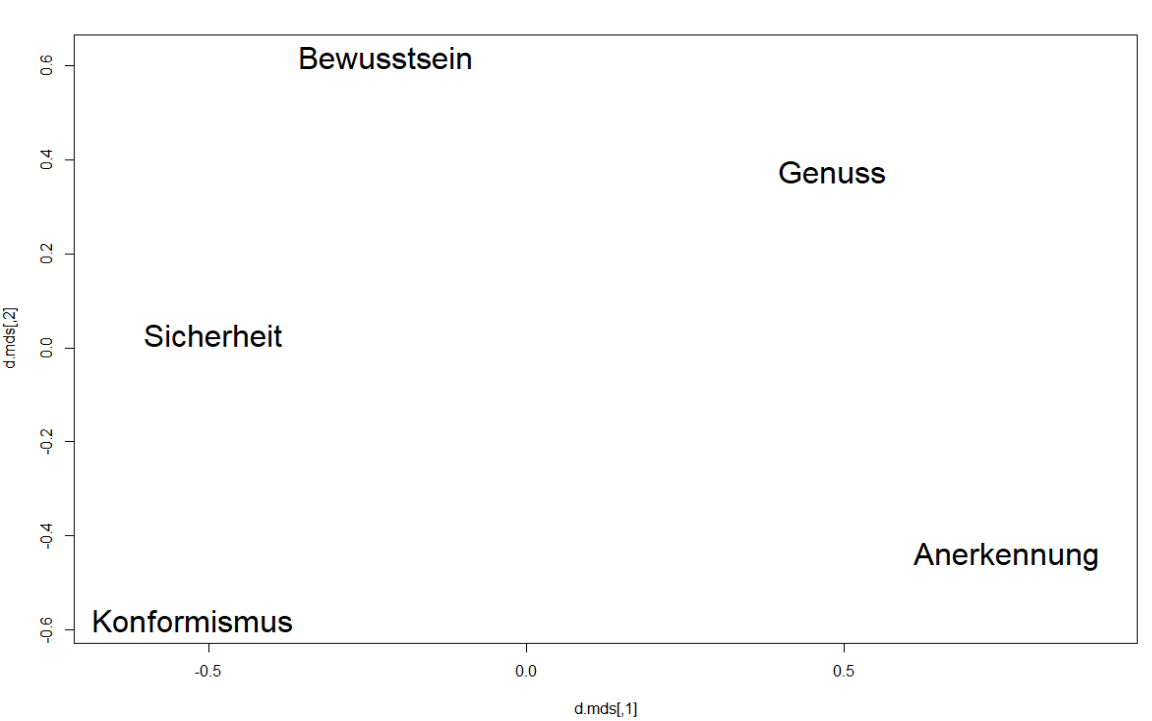
\includegraphics[width=0.8\linewidth]{./images/Marketingcontrolling/Werteraum} \end{center}

\end{frame}

\begin{frame}{Interpretation der Konfiguration der MDS}
\protect\hypertarget{interpretation-der-konfiguration-der-mds}{}

Die Interpretation der Konfiguration einer MDS kann über die Struktur
des Wahrnehmungsraumes der Befragten erfolgen. Die zusätzliche Messung
des Einkaufsverhaltens über ein \textbf{Vektormodell} nützt bei der
Interpretation der Konfiguration.

\begin{itemize}
\tightlist
\item
  Zunächst wurden die Dimensionen des Einkaufsverhaltens mit den
  Wertorientierungen korreliert.
\item
  Anschließend wurde für jede der Dimensionen des Einkaufsverhaltens
  eine lineare Regressionsanalyse durchgeführt.
\item
  Die beiden Koordinaten der Werte aus dem Werteraum in der MDS sind
  dabei die unabhängigen Variablen, anhand derer die Varianz der
  Dimension des Einkaufsverhaltens (hier die Korrelation mit den Werten)
  erklärt werden soll.
\item
  Für das Vektormodell werden die Beta-Koeffizienten der beiden
  Dimensionen für den zu zeichnenden Vektor verwendet.
\item
  Der Vektor verläuft im Diagramm als Gerade durch den Ursprung und den
  Punkt, der durch diese beiden Koordinaten festgelegt ist, und zwar als
  Pfeil in Richtung des Punktes.
\end{itemize}

\end{frame}

\begin{frame}{Ergebnisse der Regressionanalysen}
\protect\hypertarget{ergebnisse-der-regressionanalysen}{}

\begin{longtable}[]{@{}llll@{}}
\toprule
Dimension & R Square & Beta (DIM1) & Beta (DIM2)\tabularnewline
\midrule
\endhead
Brand.Conscious & 0.9038 & 0.15405 & -0.26359\tabularnewline
Novelty.Fashion & 0.7254 & 0.19014 & 0.11411\tabularnewline
Stress & 0.6918 & -0.005593 & -0.126960\tabularnewline
Impulsive & 0.7879 & 0.17578 & 0.02792\tabularnewline
Confused & 0.845 & -0.11991 & -0.09775\tabularnewline
Price & 0.9989 & -0.197832 & 0.012018\tabularnewline
Pefectionistic & 0.3836 & 0.06585 & 0.06182\tabularnewline
Habitual & 0.2503 & -0.0576 & 0.0016\tabularnewline
\bottomrule
\end{longtable}

Die standardisierten Beta-Koeffizienten geben in der Höhe ihres Betrages
Aufschluss über die Erklärkraft der einzelnen Dimensionen. Das R Square
gibt Aufschluss darüber, wie gut die Konfiguration der Objekte
(repräsentiert durch die beiden Dimensionen) geeignet ist, die Varianz
der entsprechenden Eigenschaftsbeurteilung zu erklären.

\end{frame}

\begin{frame}{Verhaltensmodell}
\protect\hypertarget{verhaltensmodell}{}

\begin{center}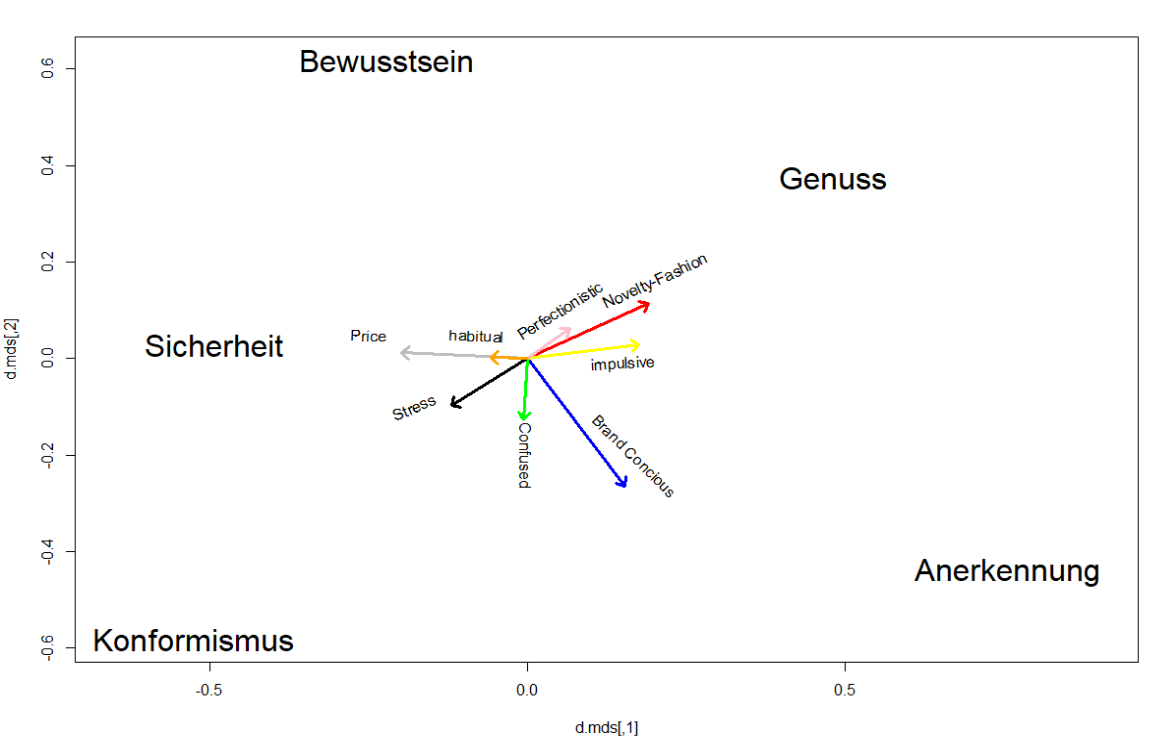
\includegraphics[width=0.8\linewidth]{./images/Marketingcontrolling/Verhaltensmodell} \end{center}

\end{frame}

\begin{frame}{Interpretation des Werteraums durch Vektoren}
\protect\hypertarget{interpretation-des-werteraums-durch-vektoren}{}

Bei der Interpretation kommt es nicht auf die Nähe der Werte zu den
Vektoren an, sondern auf die Lage des Lots\footnote<.->{Ein Lot ist in
  der Geometrie eine Strecke oder Gerade, die auf einer gegebenen
  Geraden oder Ebene senkrecht steht.} von den Werten auf den Vektor.

\begin{itemize}
\tightlist
\item
  So sind markenbewusste Käufer eher Menschen, denen Anerkennung wichtig
  sind.
\item
  Menschen mit großem Bewusstsein hingegen sind genau das Gegenteil,
  eben nicht Markenbewusst.
\item
  Genussmenschen sind Neuheits- und Modebewusst, aber auch impulsiv.\\
\item
  Menschen mit starkem Bewusstsein, wissen genau was sie wollen und
  lassen sich nicht verwirren.
\item
  Konformisten und Sicherheitsliebende macht Einkaufen keine Freude, sie
  sind dann gestresst, aber sie sind ausgesprochen preisbewusst.
\end{itemize}

\end{frame}

\begin{frame}{Konsumentensegmentierung}
\protect\hypertarget{konsumentensegmentierung}{}

\textbf{Zielsetzung} Im Rahmen einer Konsumentensegmentierung wird der
Gesamtmarkt in Konsumentensegmente unterteilt. Ein Konsumentensegment
wird dabei als eine möglichst homogene Gruppe von Konsumenten
verstanden. Ein Unternehmen kann sich dann entscheiden, welche Segmente
es bearbeiten will.

\textbf{Praktische Anwendung} Marktforschung, Produktneugestaltung,
Positionierung, Werbung, Imagebildung, etc. pp.

\textbf{Umsetzung} Als Segmentierungskriterien werden Werte und
Wertorientierungen als psychographische Segemntierungskriterien und das
Einkaufsverhalten als verhaltensbezogene Segmentierungskriterien
verwendet.

\textbf{Ergebniss} Mittels Clusteranalyse lassen sich sodann sieben
Verhaltenstypen (das CHOUGHS-Modell) identifizieren.

\end{frame}

\begin{frame}{Das CHOUGHS-Modell (Krähen-Modell)}
\protect\hypertarget{das-choughs-modell-krahen-modell}{}

\begin{center}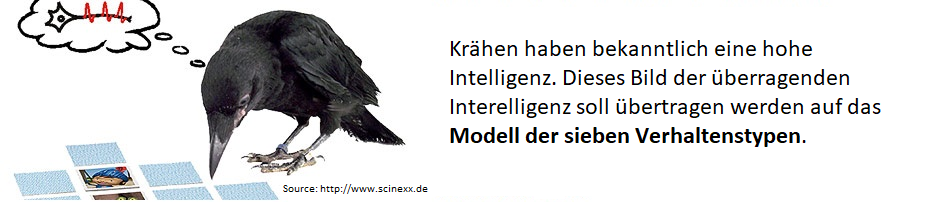
\includegraphics[width=0.8\linewidth]{./images/Marketingcontrolling/choughs} \end{center}

Das Acronym CHOUGHS (engl. Krähe) passt hier sehr gut zu den
Anfangsbuchstaben der sieben Verhaltenstypen:

\textbf{C} onformism (Konformisten)\\
\textbf{H} endonism (Hedonisten)\\
\textbf{O} ut of responsibility (Verantwortungsverweigerer)\\
\textbf{U} nderstand (Werschätzende)\\
\textbf{G} ourmets (Genießer)\\
\textbf{H} armony (Harmoniesuchende)\\
\textbf{S} elf-determined (Selbstbestimmte)

\end{frame}

\begin{frame}[shrink]{Die sieben FOM-Verhaltenstypen}
\protect\hypertarget{die-sieben-fom-verhaltenstypen}{}

\begin{center}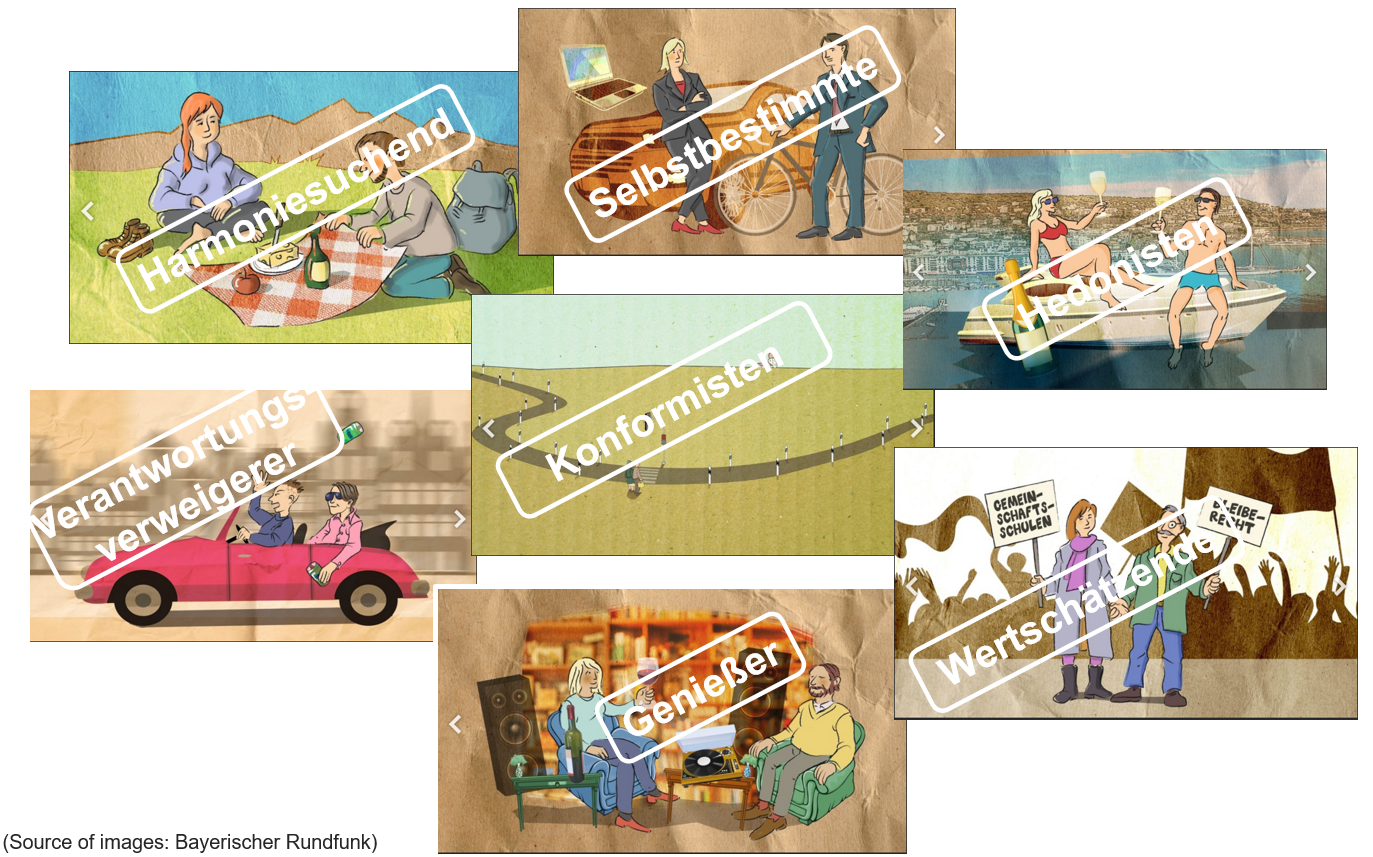
\includegraphics[width=0.8\linewidth]{./images/Marketingcontrolling/Verhaltenstypen} \end{center}

Sind die Verhhaltenstypen bekannt, können schnell und zuverlässig
Verhaltensweisen abgeleitet werden.

\end{frame}

\begin{frame}[shrink]{Wertorientierungen und Einkaufsverhalten im
CHOUGHS-Modell}
\protect\hypertarget{wertorientierungen-und-einkaufsverhalten-im-choughs-modell}{}

Die Ausprägung je Verhaltenstyp über die 5 Werte- und 8
Einkaufsverhaltensdimensionen lassen sich sehr gut über ein
\textbf{Heatmap} ablesen. Dunkle Felder stehen für hohe Ausprägung und
helle Felder für niedrige Ausprägung bezüglich Dimension und Typ.

\begin{center}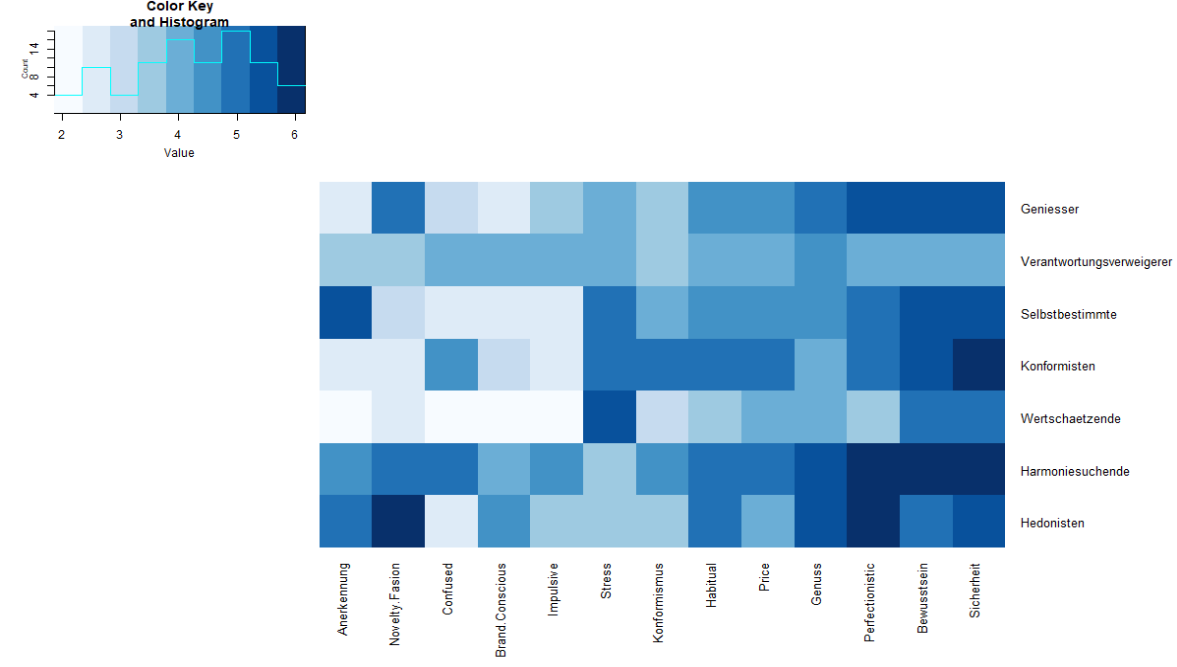
\includegraphics[width=0.8\linewidth]{./images/Marketingcontrolling/Heatmap} \end{center}

\end{frame}

\begin{frame}{Übung 36: Hedonisten}
\protect\hypertarget{ubung-36-hedonisten}{}

Welche Eigenschaften würden Sie einem Hedonsiten zuschreiben?

\begin{enumerate}
[A.]
\tightlist
\item
  Kein Interesse an Markenartikeln.
\item
  Nicht perfektionistisch.
\item
  Extrem Neuheits- und Modebewusst.
\item
  Anerkennung ist nicht wichtig.
\end{enumerate}

\note{\textbf{\emph{C}}}

\end{frame}

\begin{frame}{Biplot der Mittelwerte der Input-Daten}
\protect\hypertarget{biplot-der-mittelwerte-der-input-daten}{}

Ein \textbf{Biplot} für die Mittelwerte aller Werte- und
Einkaufsverhaltensdimensionen ergibt ein interpretierbares Bild
(Wahrnehmungsraum).

Es werden sodann zwei Biplots gerechnet, einmal für \textbf{Werte} und
einmal für das \textbf{Einkaufsverhalten}.

Die beiden Räume zeigen, wo sich die Typen in Bezug auf die Dimensionen
befinden. Beide Räume zeigen die gleichen Ergebnisse wie zuvor das
Theoretische Modell und die Clusteranalyse.

In der Marktforschung sind Modelle dann gut, wenn die Daten mit
verschiedenen Analyseinstumenten gleiche Ergebnisse zeigen. Das ist hier
der Fall.

\end{frame}

\begin{frame}[shrink]{Werteraum isoliert betrachtet}
\protect\hypertarget{werteraum-isoliert-betrachtet}{}

\begin{center}\includegraphics[width=0.8\linewidth]{./images/Marketingcontrolling/Werteverhaltensraum} \end{center}

\end{frame}

\begin{frame}[shrink]{Einkaufverhaltensraum isoliert betrachtet}
\protect\hypertarget{einkaufverhaltensraum-isoliert-betrachtet}{}

\begin{center}\includegraphics[width=0.8\linewidth]{./images/Marketingcontrolling/Einkaufverhaltensraum} \end{center}

\end{frame}

\begin{frame}{Übung 37: Einsatz des Modells}
\protect\hypertarget{ubung-37-einsatz-des-modells}{}

Für welche Zwecke können Sie das Modell in der Praxis einsetzen?

\begin{enumerate}
[A.]
\tightlist
\item
  Kundenclusterung.
\item
  Neuproduktentwicklung.
\item
  Positionierung.
\item
  Alle Antworten sind richtig.
\end{enumerate}

\note{\textbf{\emph{D}}}

\end{frame}

\begin{frame}{Übung 38: Anwendung des Modells}
\protect\hypertarget{ubung-38-anwendung-des-modells}{}

Diskutieren Sie mögliche Einsatzgebiete und Anwendungsmöglichkeiten für
das eigene Unternehmen.

\note{Heinweis: Für den Einsatz und die Anwendung des validierten
CHOUGHS-Modells (sowohl für die Forschung, als auch für die Praxis)
benötigen Sie einen Kurzfragebogen, den Sie über das ifes bekommen:

Prof.~Dr.~Oliver Gansser - Mail:
\href{mailto:oliver.gansser@fom-ifes.de}{\nolinkurl{oliver.gansser@fom-ifes.de}}\\
ifes Institut für Empirie \& Statistik\\
Arnulfstraße 30\\
80335 München}

\end{frame}

\begin{frame}{Literatur}
\protect\hypertarget{literatur-4}{}

\begin{itemize}
\tightlist
\item
  Davidov, E., Schmidt, P., \& Schwartz, S.\thinspace{}H. (2008).
  Bringing values back in: The adequacy of the European social survey to
  measure values in 20 countries. Public Opin. Q., 72(3),
  S.\thinspace{}420--445.
\item
  Kluckhohn, C. (1951). Values and Value-Orientations in the theory of
  action, in: Toward a General Theory of Action (Hrsg.: v. Parsons,
  Talcott /\thinspace{}Shils, Edward
  \mbox{A.\thinspace{}S.),}\xspace{}\thinspace{}S.\thinspace{}388--433.
\item
  Lovejoy, A.\thinspace{}O. (1950). Terminal and adjectival values. J.
  Philos., 47, S.\thinspace{}593--608.
\item
  Rokeach, M. (1973). The Nature of Human Values, New York.
\item
  Schmidt, P., Bamberg, S., Davidov, E., Herrmann, J., \& Schwartz,
  S.\thinspace{}H. (2007). Die Messung von Werten mit dem ``Portraits
  Value Questionnaire''. Zeitschrift für Sozialpsychologie, 38(4),
  S.\thinspace{}261--275.
\item
  Smith, M.\thinspace{}B. (1969). Social psychology and human values,
  Chicago.
\item
  Sproles, G.\thinspace{}B., \& Kendal, E.\thinspace{}L. (1986). A
  Methodology for Profiling Consumers' Decision-Making Styles. J.
  Consum. Aff., 20(2), 267--279.
\item
  Williams, R.\thinspace{}M. (1968). Values, in: Int. Encycl. Soc. Sci.,
  S.\thinspace{}286--287, New York.
\end{itemize}

\end{frame}

\hypertarget{warenkorbanalyse}{%
\section{Warenkorbanalyse}\label{warenkorbanalyse}}

\begin{frame}{Lernziele}
\protect\hypertarget{lernziele-8}{}

\begin{itemize}
\tightlist
\item
  Einsatz und Ziel der Warenkorbanalyse verstehen.
\item
  Daten für die Warenkorbanalyse einlesen.
\item
  Anwendung der Warenkorbanalyse.
\item
  Interpretation und Schlussfolgerungen der Warenkorbanalyse.
\item
  Evaluation des Einsates der Warenkorbanalyse in der Marketing
  Controlling Praxis.
\end{itemize}

\end{frame}

\begin{frame}{Warenkorbanalyse}
\protect\hypertarget{warenkorbanalyse-1}{}

Die Warenkorbanalyse ist eine Methode, die die beim Einkauf gemeinsam
gekauften Produkte oder Produktkategorien aus einem Handelssortiment
untersucht.

\textbf{Ziel}\\
Strukturen in den Daten finden, so genannte Regeln, die beschreiben,
welche Produkte oder Produktkategorien gemeinsam oder eben nicht
gemeinsam gekauft werden.

\textbf{Beispiel}\\
Wenn ein Kunde Windeln und Bier kauft, kauft er auch Chips.

\textbf{Methode}\\
\emph{Assoziationsanalyse} - oder auch \textbf{Warenkorbanalyse}.

\textbf{Anwendung}\\
Werden solche Regeln gefunden, kann das Ergebnis beispielsweise für
Verbundplatzierungen im Verkaufsraum oder in der Werbung verwendet
werden.

\end{frame}

\begin{frame}[fragile,shrink]{Laden der Pakete und Download der Daten}
\protect\hypertarget{laden-der-pakete-und-download-der-daten}{}

\begin{Shaded}
\begin{Highlighting}[]
\KeywordTok{library}\NormalTok{(mosaic)}
\KeywordTok{library}\NormalTok{(arules)}
\KeywordTok{library}\NormalTok{(arulesViz)}

\CommentTok{# Laden Datensatz}
\KeywordTok{data}\NormalTok{(Groceries)}

\CommentTok{# Dataframe aus Transaktionsdaten generieren }
\NormalTok{groceries<-}\KeywordTok{as}\NormalTok{(Groceries, }\StringTok{'data.frame'}\NormalTok{)}
\end{Highlighting}
\end{Shaded}

\end{frame}

\begin{frame}[fragile,shrink]{Betrachten der Daten}
\protect\hypertarget{betrachten-der-daten}{}

\begin{Shaded}
\begin{Highlighting}[]
\CommentTok{# Betrachten der Warengruppen der ersten 6 Transaktionen}
\NormalTok{groceries[}\DecValTok{1}\OperatorTok{:}\DecValTok{6}\NormalTok{,]}
\end{Highlighting}
\end{Shaded}

\begin{verbatim}
## [1] {citrus fruit,semi-finished bread,margarine,ready soups}             
## [2] {tropical fruit,yogurt,coffee}                                       
## [3] {whole milk}                                                         
## [4] {pip fruit,yogurt,cream cheese ,meat spreads}                        
## [5] {other vegetables,whole milk,condensed milk,long life bakery product}
## [6] {whole milk,butter,yogurt,rice,abrasive cleaner}                     
## 7011 Levels: {abrasive cleaner,napkins} ... {zwieback}
\end{verbatim}

\end{frame}

\begin{frame}[fragile,shrink]{Datenaufbau}
\protect\hypertarget{datenaufbau}{}

\begin{Shaded}
\begin{Highlighting}[]
\KeywordTok{summary}\NormalTok{(Groceries)}
\end{Highlighting}
\end{Shaded}

\begin{verbatim}
## transactions as itemMatrix in sparse format with
##  9835 rows (elements/itemsets/transactions) and
##  169 columns (items) and a density of 0.02609146 
## 
## most frequent items:
##       whole milk other vegetables       rolls/buns             soda 
##             2513             1903             1809             1715 
##           yogurt          (Other) 
##             1372            34055 
## 
## element (itemset/transaction) length distribution:
## sizes
##    1    2    3    4    5    6    7    8    9   10   11   12   13   14 
## 2159 1643 1299 1005  855  645  545  438  350  246  182  117   78   77 
##   15   16   17   18   19   20   21   22   23   24   26   27   28   29 
##   55   46   29   14   14    9   11    4    6    1    1    1    1    3 
##   32 
##    1 
## 
##    Min. 1st Qu.  Median    Mean 3rd Qu.    Max. 
##   1.000   2.000   3.000   4.409   6.000  32.000 
## 
## includes extended item information - examples:
##        labels  level2           level1
## 1 frankfurter sausage meat and sausage
## 2     sausage sausage meat and sausage
## 3  liver loaf sausage meat and sausage
\end{verbatim}

\end{frame}

\begin{frame}{Interpretation der Zusammenfassung}
\protect\hypertarget{interpretation-der-zusammenfassung}{}

\begin{enumerate}
\item
  Bei dem Datensatz handelt es sich um Transaktionsdaten mit 9835
  Transaktionen und 169 Warengruppen (items).
\item
  Auflistung der fünf am häufigsten gekauften Warengruppen mit der
  Anzahl der Transaktionen, in denen sie vorkommen.
\item
  Verteilung der „Länge`` der Transaktionen.
\item
  Zusätzlich zu den Bezeichnungen der Warengruppen (labels) sind
  Informationen zur Sortimentshierarchie vorhanden sind (level1 und
  level2).
\end{enumerate}

\end{frame}

\begin{frame}[fragile,shrink]{Länge der Transaktionen}
\protect\hypertarget{lange-der-transaktionen}{}

\begin{Shaded}
\begin{Highlighting}[]
\CommentTok{# Welche Transaktionen sind größer 25?}
\KeywordTok{which}\NormalTok{(}\KeywordTok{size}\NormalTok{(Groceries) }\OperatorTok{>}\StringTok{ }\DecValTok{25}\NormalTok{)}
\end{Highlighting}
\end{Shaded}

\begin{verbatim}
## [1] 1092 1217 2939 2974 4431 5611 9002
\end{verbatim}

\begin{Shaded}
\begin{Highlighting}[]
\CommentTok{# Histogramm der Transaktionslängen}
\KeywordTok{hist}\NormalTok{(}\KeywordTok{size}\NormalTok{(Groceries))}
\end{Highlighting}
\end{Shaded}

\begin{center}\includegraphics{Marketing-Controlling_files/figure-beamer/unnamed-chunk-97-1} \end{center}

\end{frame}

\begin{frame}[fragile,shrink]{Häufigste Warengruppen}
\protect\hypertarget{haufigste-warengruppen}{}

\begin{Shaded}
\begin{Highlighting}[]
\CommentTok{# Relative Häufigkeiten der häufigsten Produkte, }
\CommentTok{# hier nach relativer Häufigkeit größer 0,1 gefiltert.}
\KeywordTok{itemFrequencyPlot}\NormalTok{(Groceries, }\DataTypeTok{support=}\FloatTok{0.1}\NormalTok{)}
\end{Highlighting}
\end{Shaded}

\begin{center}\includegraphics{Marketing-Controlling_files/figure-beamer/unnamed-chunk-98-1} \end{center}

\end{frame}

\begin{frame}[fragile,shrink]{Die 20 häufigsten Warengruppen}
\protect\hypertarget{die-20-haufigsten-warengruppen}{}

\begin{Shaded}
\begin{Highlighting}[]
\KeywordTok{itemFrequencyPlot}\NormalTok{(Groceries, }\DataTypeTok{topN=}\DecValTok{20}\NormalTok{)}
\end{Highlighting}
\end{Shaded}

\begin{center}\includegraphics{Marketing-Controlling_files/figure-beamer/unnamed-chunk-99-1} \end{center}

\end{frame}

\begin{frame}{Assoziationsanalyse}
\protect\hypertarget{assoziationsanalyse}{}

Im nächsten Schritt wird mit statistischen Methoden nach Strukturen in
den Daten gesucht. Als Grundlage werden \textbf{Ähnlichkeitsmatrizen}
erstellt, die für jedes Warengruppenpaar die Häufigkeit des gemeinsamen
Vorkommens in Transaktionen bestimmen.

Solch eine \textbf{Ähnlichkeitsmatrix} ist zum Beispiel eine
\textbf{Kreuztabelle} in der es für jedes Produkt eine Spalte und eine
Zeile gibt.

In den Zellen in der Tabelle steht jeweils die Häufigkeit, wie oft
dieses Produktpaar gemeinsam in Transaktionen in den Daten vorkommt.

\end{frame}

\begin{frame}[fragile,shrink]{Häufigkeiten der gemeinsamen Käufe}
\protect\hypertarget{haufigkeiten-der-gemeinsamen-kaufe}{}

\begin{Shaded}
\begin{Highlighting}[]
\CommentTok{# Kreuztabelle als ct speichern}
\NormalTok{ct<-}\KeywordTok{crossTable}\NormalTok{(Groceries)}

\CommentTok{# Ausgabe der Zeilen 1:5 und Spalten 14:17 (Bsp.)}
\NormalTok{ct[}\DecValTok{1}\OperatorTok{:}\DecValTok{5}\NormalTok{,}\DecValTok{14}\OperatorTok{:}\DecValTok{17}\NormalTok{]}
\end{Highlighting}
\end{Shaded}

\begin{verbatim}
##             citrus fruit tropical fruit pip fruit grapes
## frankfurter           64             93        71     21
## sausage              111            137       106     31
## liver loaf             5              6         9      2
## ham                   28             53        39     13
## meat                  34             33        27      5
\end{verbatim}

=\textgreater{} Frankfurter und Zitrusfrüchte werden in 64 Transaktionen
zusammen gekauft, Frankfurter und grapes in 21 usw.

\end{frame}

\begin{frame}{Clusteranalyse}
\protect\hypertarget{clusteranalyse}{}

Auf Basis der \textbf{Ähnlichkeitsmatrix} wird dann
\mbox{z.\thinspace{}B.}\xspace{} mit Mehrdimensionaler Skalierung oder
hierarchischen Clusteranalysen nach Strukturen in den Daten gesucht.

Die \textbf{hierarchische Clusteranalyse} liefert dann ein Dendrogram,
siehe folgende Abbildung, in der ähnliche Produkte miteinander gruppiert
indentifiziert werden können.

Ähnliche Produkte (also Produkte, die zusammen gekauft werden) werden
zusammen in Gruppen geclustert. Je länger die vertikale Verbindungslinie
ist, die zwei Warengruppen zusammenfasst, um so unterschiedlicher sind
diese.

\end{frame}

\begin{frame}[fragile,shrink]{Dendrogram}
\protect\hypertarget{dendrogram}{}

\begin{Shaded}
\begin{Highlighting}[]
\NormalTok{diss <-}\StringTok{ }\KeywordTok{dissimilarity}\NormalTok{(Groceries[, }\KeywordTok{itemFrequency}\NormalTok{(Groceries) }\OperatorTok{>}\StringTok{ }\FloatTok{0.03}\NormalTok{],}
\DataTypeTok{method =} \StringTok{"Jaccard"}\NormalTok{, }\DataTypeTok{which =} \StringTok{"items"}\NormalTok{) }
\NormalTok{hc <-}\StringTok{ }\KeywordTok{hclust}\NormalTok{(diss, }\DataTypeTok{method =} \StringTok{"ward.D"}\NormalTok{)}
\KeywordTok{plot}\NormalTok{(hc)}
\end{Highlighting}
\end{Shaded}

\begin{center}\includegraphics{Marketing-Controlling_files/figure-beamer/unnamed-chunk-101-1} \end{center}

\end{frame}

\begin{frame}[shrink]{Assoziationsregeln}
\protect\hypertarget{assoziationsregeln}{}

Es werden Regeln gesucht und an den Daten geprüft, die das Kaufverhalten
der Kunden beschreiben.

Solch eine Regel ist zum Beispiel „Wenn ein Kunde Windeln und Bier
kauft, kauft er auch Chips.``

Für diese Regeln lassen sich statistische Maßzahlen berechnen, die die
Güte und Bedeutung der Regeln beschreiben:

\textbf{Support} ist das Signifikanzmaß der Regel. Es gibt an, wie oft
die gefundene Regel in den Daten anzuwenden ist. Bsp.: Wie oft kommen
Windeln, Bier und Chips in einer Transaktion gemeinsam vor?

\textbf{Confidence} ist das Qualitätsmaß der Regel. Es beschreibt, wie
oft die Regel richtig ist. Bsp.: Wie oft ist in einer Transaktion Chips
enthalten, wenn auch Windeln und Bier enthalten sind?

\textbf{Lift} ist das Maß der Bedeutung der Regel. Es sagt aus wie oft
die Confidence den Erwartungswert übersteigt. Bsp.: Wie ist die
Häufigkeit des gemeinsamen Vorkommens von Windeln, Bier und Chips im
Verhältlnis zur erwarteten Häufigkeit des Vorkommens, wenn die
Ereignisse stochastisch unabhängig sind?

\end{frame}

\begin{frame}{Übung 39: Vergleich Support und Confidence}
\protect\hypertarget{ubung-39-vergleich-support-und-confidence}{}

Stimmt die Aussage: Die Confidenz ist stets größer als der Support:
\emph{Confidence}(\(A \rightarrow B\))\textgreater{}\emph{Support}(\(B\))?

\begin{itemize}
\tightlist
\item
  Ja.
\item
  Nein.
\end{itemize}

\note{\textbf{\emph{Nein}}, nur wenn \emph{Lift}\textgreater{}1:
z.\thinspace{}B. könnten \(10\,\%\) aller Kunden Gemüse kaufen, aber nur
\(5\,\%\) aller Kunden von Korn.}

\end{frame}

\begin{frame}{Algorithmen}
\protect\hypertarget{algorithmen}{}

In den Daten werden zunächst alle möglichen \textbf{Regeln} gesammelt,
die einen Mindestwert an Support und Confidence haben. Die Mindestwerte
werden dabei vom Nutzer vorgegeben. Da es sich bei Transaktionsdaten um
große Datenmengen handelt und häufig große Anzahlen von Produkten
enthalten sind, wird die Suche nach Regeln zu einem komplexen Problem.

Sind die \textbf{Assoziationsregeln} gefunden, können Sie vom Nutzer
genauer untersucht werden und \mbox{z.\thinspace{}B.}\xspace{} nach den
oben genannten Kennzahlen sortiert betrachtet werden, oder es werden die
Regeln für spezielle Warenkategorien genauer betrachtet.

\end{frame}

\begin{frame}[fragile,shrink]{Regeln}
\protect\hypertarget{regeln}{}

\begin{Shaded}
\begin{Highlighting}[]
\KeywordTok{apriori}\NormalTok{(Groceries)}
\end{Highlighting}
\end{Shaded}

\begin{verbatim}
## Apriori
## 
## Parameter specification:
##  confidence minval smax arem  aval originalSupport maxtime support
##         0.8    0.1    1 none FALSE            TRUE       5     0.1
##  minlen maxlen target   ext
##       1     10  rules FALSE
## 
## Algorithmic control:
##  filter tree heap memopt load sort verbose
##     0.1 TRUE TRUE  FALSE TRUE    2    TRUE
## 
## Absolute minimum support count: 983 
## 
## set item appearances ...[0 item(s)] done [0.00s].
## set transactions ...[169 item(s), 9835 transaction(s)] done [0.00s].
## sorting and recoding items ... [8 item(s)] done [0.00s].
## creating transaction tree ... done [0.00s].
## checking subsets of size 1 2 done [0.00s].
## writing ... [0 rule(s)] done [0.00s].
## creating S4 object  ... done [0.00s].
\end{verbatim}

\begin{verbatim}
## set of 0 rules
\end{verbatim}

\end{frame}

\begin{frame}[fragile,shrink]{Regeln mit Limitationen}
\protect\hypertarget{regeln-mit-limitationen}{}

\begin{Shaded}
\begin{Highlighting}[]
\CommentTok{# Support, confidence und minimale Länge festlegen}
\NormalTok{grules<-}\KeywordTok{apriori}\NormalTok{(Groceries, }\DataTypeTok{parameter =} \KeywordTok{list}\NormalTok{(}\DataTypeTok{support =} \FloatTok{0.009}\NormalTok{, }\DataTypeTok{confidence =} \FloatTok{0.25}\NormalTok{, }\DataTypeTok{minlen =} \DecValTok{2}\NormalTok{))}
\end{Highlighting}
\end{Shaded}

\begin{verbatim}
## Apriori
## 
## Parameter specification:
##  confidence minval smax arem  aval originalSupport maxtime support
##        0.25    0.1    1 none FALSE            TRUE       5   0.009
##  minlen maxlen target   ext
##       2     10  rules FALSE
## 
## Algorithmic control:
##  filter tree heap memopt load sort verbose
##     0.1 TRUE TRUE  FALSE TRUE    2    TRUE
## 
## Absolute minimum support count: 88 
## 
## set item appearances ...[0 item(s)] done [0.00s].
## set transactions ...[169 item(s), 9835 transaction(s)] done [0.00s].
## sorting and recoding items ... [93 item(s)] done [0.00s].
## creating transaction tree ... done [0.00s].
## checking subsets of size 1 2 3 4 done [0.00s].
## writing ... [224 rule(s)] done [0.00s].
## creating S4 object  ... done [0.00s].
\end{verbatim}

\begin{Shaded}
\begin{Highlighting}[]
\NormalTok{grules}
\end{Highlighting}
\end{Shaded}

\begin{verbatim}
## set of 224 rules
\end{verbatim}

\end{frame}

\begin{frame}[fragile]{Übung 40: Limitation}
\protect\hypertarget{ubung-40-limitation}{}

Was passiert, wenn der minimale Support erhöht wird, z.\thinspace{}B.
\texttt{supp=0.02}?

\begin{enumerate}
[A.]
\tightlist
\item
  Es werden weniger Regeln gefunden.
\item
  Es werden mehr Regeln gefunden.
\item
  Es werden genauso viele Regeln gefunden.
\end{enumerate}

\note{\textbf{\emph{A}} Im Beispiel wird statt 224 Regeln nur noch 49
gefunden.}

\end{frame}

\begin{frame}[fragile,shrink]{Bewertung der Regeln}
\protect\hypertarget{bewertung-der-regeln}{}

\begin{Shaded}
\begin{Highlighting}[]
\KeywordTok{summary}\NormalTok{(grules)}
\end{Highlighting}
\end{Shaded}

\begin{verbatim}
## set of 224 rules
## 
## rule length distribution (lhs + rhs):sizes
##   2   3 
## 111 113 
## 
##    Min. 1st Qu.  Median    Mean 3rd Qu.    Max. 
##   2.000   2.000   3.000   2.504   3.000   3.000 
## 
## summary of quality measures:
##     support           confidence          lift            count      
##  Min.   :0.009049   Min.   :0.2513   Min.   :0.9932   Min.   : 89.0  
##  1st Qu.:0.010066   1st Qu.:0.2974   1st Qu.:1.5767   1st Qu.: 99.0  
##  Median :0.012303   Median :0.3603   Median :1.8592   Median :121.0  
##  Mean   :0.016111   Mean   :0.3730   Mean   :1.9402   Mean   :158.5  
##  3rd Qu.:0.018480   3rd Qu.:0.4349   3rd Qu.:2.2038   3rd Qu.:181.8  
##  Max.   :0.074835   Max.   :0.6389   Max.   :3.7969   Max.   :736.0  
## 
## mining info:
##       data ntransactions support confidence
##  Groceries          9835   0.009       0.25
\end{verbatim}

\end{frame}

\begin{frame}[fragile,shrink]{Analyse der Regeln}
\protect\hypertarget{analyse-der-regeln}{}

\begin{Shaded}
\begin{Highlighting}[]
\CommentTok{# Analyse der ersten 10 Regeln}
\KeywordTok{inspect}\NormalTok{(grules[}\DecValTok{1}\OperatorTok{:}\DecValTok{10}\NormalTok{])}
\end{Highlighting}
\end{Shaded}

\begin{verbatim}
##      lhs                rhs                support     confidence
## [1]  {baking powder} => {whole milk}       0.009252669 0.5229885 
## [2]  {grapes}        => {other vegetables} 0.009049314 0.4045455 
## [3]  {meat}          => {other vegetables} 0.009964413 0.3858268 
## [4]  {meat}          => {whole milk}       0.009964413 0.3858268 
## [5]  {frozen meals}  => {whole milk}       0.009862735 0.3476703 
## [6]  {hard cheese}   => {other vegetables} 0.009456024 0.3858921 
## [7]  {hard cheese}   => {whole milk}       0.010066090 0.4107884 
## [8]  {butter milk}   => {other vegetables} 0.010371124 0.3709091 
## [9]  {butter milk}   => {whole milk}       0.011591256 0.4145455 
## [10] {ham}           => {other vegetables} 0.009150991 0.3515625 
##      lift     count
## [1]  2.046793  91  
## [2]  2.090754  89  
## [3]  1.994013  98  
## [4]  1.509991  98  
## [5]  1.360659  97  
## [6]  1.994350  93  
## [7]  1.607682  99  
## [8]  1.916916 102  
## [9]  1.622385 114  
## [10] 1.816930  90
\end{verbatim}

\end{frame}

\begin{frame}{Regelanalyse Interpretation}
\protect\hypertarget{regelanalyse-interpretation}{}

Regeln sollten nicht einfach unreflektiert übernommen werden.

Grundsätzlich sollte man unterscheiden zwischen:

\textbf{Handlungsfähigkeit}\\
Regeln sollten einen klaren und nützlichen Einblick in die Realität
bieten.

\textbf{Trivial}\\
Alle Regeln, die so offensichtlich sind, dass sie nicht erwähnenswert
sind, sind klar, aber nicht nützlich.

\textbf{Unerklärlichkeit}\\
Wenn der Zusammenhang zwischen den Elementen so unklar ist, dass es
zusätzlicher Forschung bedarf, um herauszufinden, wie die Informationen
für Aktionen genutzt werden können.

\end{frame}

\begin{frame}[fragile,shrink]{Analyse der Top5 Regeln}
\protect\hypertarget{analyse-der-top5-regeln}{}

\begin{Shaded}
\begin{Highlighting}[]
\CommentTok{# Welches sind die top 5 Regeln?  }
\NormalTok{top5<-}\KeywordTok{sort}\NormalTok{(grules, }\DataTypeTok{by =} \StringTok{"lift"}\NormalTok{)[}\DecValTok{1}\OperatorTok{:}\DecValTok{5}\NormalTok{]}
\KeywordTok{inspect}\NormalTok{(top5)}
\end{Highlighting}
\end{Shaded}

\begin{verbatim}
##     lhs                   rhs                      support confidence     lift count
## [1] {berries}          => {whipped/sour cream} 0.009049314  0.2721713 3.796886    89
## [2] {tropical fruit,                                                                
##      other vegetables} => {pip fruit}          0.009456024  0.2634561 3.482649    93
## [3] {pip fruit,                                                                     
##      other vegetables} => {tropical fruit}     0.009456024  0.3618677 3.448613    93
## [4] {citrus fruit,                                                                  
##      other vegetables} => {root vegetables}    0.010371124  0.3591549 3.295045   102
## [5] {tropical fruit,                                                                
##      other vegetables} => {root vegetables}    0.012302999  0.3427762 3.144780   121
\end{verbatim}

\end{frame}

\begin{frame}{Übung 41: Interpretation Support}
\protect\hypertarget{ubung-41-interpretation-support}{}

Wie lautet die richtige Interpretation von \emph{Support}(\{citrus
fruit,other vegetables\} =\textgreater{} \{root
vegetables\})=0.012302999?

\begin{enumerate}
[A.]
\tightlist
\item
  0.010371124 aller Transaktionen enthalten \{citrus fruit,other
  vegetables\} oder \{root vegetables\}.
\item
  0.010371124 aller Transaktionen enthalten \{citrus fruit,other
  vegetables\} und \{root vegetables\}.
\item
  0.010371124 der Transaktionen von \{citrus fruit,other vegetables\}
  enthalten auch \{root vegetables\}.
\item
  0.010371124 der Transaktionen von \{root vegetables\} enthalten auch
  \{citrus fruit,other vegetables\}.
\end{enumerate}

\note{\textbf{\emph{B}}}

\end{frame}

\begin{frame}{Übung 42: Interpretation Confidence}
\protect\hypertarget{ubung-42-interpretation-confidence}{}

Wie lautet die richtige Interpretation von \emph{Confidence}(\{citrus
fruit,other vegetables\} =\textgreater{} \{root vegetables\})=0.3591549?

\begin{enumerate}
[A.]
\tightlist
\item
  0.3591549 aller Transaktionen enthalten \{citrus fruit,other
  vegetables\} oder \{root vegetables\}.
\item
  0.3591549 aller Transaktionen enthalten \{citrus fruit,other
  vegetables\} und \{root vegetables\}.
\item
  0.3591549 der Transaktionen von \{citrus fruit,other vegetables\}
  enthalten auch \{root vegetables\}.
\item
  0.3591549 der Transaktionen von \{root vegetables\} enthalten auch
  \{citrus fruit,other vegetables\}.
\end{enumerate}

\note{\textbf{\emph{C}}}

\end{frame}

\begin{frame}{Übung 43: Interpretation Lift}
\protect\hypertarget{ubung-43-interpretation-lift}{}

Simmt die Aussage: Kunden die \{citrus fruit,other vegetable\} kaufen,
kaufen \(3.295045\times\) häufiger \{root vegetables\} als unter
Unabhängigkeit zu erwarten wäre.

\begin{itemize}
\tightlist
\item
  Ja.
\item
  Nein.
\end{itemize}

\note{\textbf{\emph{Ja}}, \emph{Lift}(\{citrus fruit,other vegetabl\}
=\textgreater{} \{root vegetables\})=3.29504.}

\end{frame}

\begin{frame}[fragile,shrink]{Regeln mit hohem Support und hoher
Confidence}
\protect\hypertarget{regeln-mit-hohem-support-und-hoher-confidence}{}

\begin{Shaded}
\begin{Highlighting}[]
\KeywordTok{inspect}\NormalTok{(}\KeywordTok{sort}\NormalTok{(}\KeywordTok{sort}\NormalTok{(grules, }\DataTypeTok{by =}\StringTok{"support"}\NormalTok{),}\DataTypeTok{by =}\StringTok{"confidence"}\NormalTok{)[}\DecValTok{1}\OperatorTok{:}\DecValTok{5}\NormalTok{])}
\end{Highlighting}
\end{Shaded}

\begin{verbatim}
##     lhs                   rhs                    support confidence     lift count
## [1] {butter,                                                                      
##      yogurt}           => {whole milk}       0.009354347  0.6388889 2.500387    92
## [2] {citrus fruit,                                                                
##      root vegetables}  => {other vegetables} 0.010371124  0.5862069 3.029608   102
## [3] {tropical fruit,                                                              
##      root vegetables}  => {other vegetables} 0.012302999  0.5845411 3.020999   121
## [4] {curd,                                                                        
##      yogurt}           => {whole milk}       0.010066090  0.5823529 2.279125    99
## [5] {other vegetables,                                                            
##      curd}             => {whole milk}       0.009862735  0.5739645 2.246296    97
\end{verbatim}

\end{frame}

\begin{frame}{Übung 44: Relevanz}
\protect\hypertarget{ubung-44-relevanz}{}

Woran können Sie am ehesten erkennen, ob eine Regel relevant ist,
\mbox{d.\thinspace{}h.,}\xspace{} viele Transaktionen betrifft?

\begin{enumerate}
[A.]
\tightlist
\item
  An einem hohen Support.
\item
  An einer hohen Konfidenz.
\item
  An einem hohen Lift.
\end{enumerate}

\note{\textbf{\emph{A}}, Support, da dieser sagt, wie oft eine Regel
auftaucht.}

\end{frame}

\begin{frame}{Übung 45: Verbundwirkung}
\protect\hypertarget{ubung-45-verbundwirkung}{}

Woran können Sie am ehesten erkennen, ob es eine hohe
Assoziation\thinspace{}/\thinspace{}Verbundwirkung zwischen den Items
gibt.

\begin{enumerate}
[A.]
\tightlist
\item
  An einem hohen Support.
\item
  An einer hohen Konfidenz.
\item
  An einem hohen Lift.
\end{enumerate}

\note{\textbf{\emph{C}}, Lift, da hier die Steigerung der relativen
Häufigkeit gemessen wird.}

\end{frame}

\begin{frame}{Übung 46: Empfehlung}
\protect\hypertarget{ubung-46-empfehlung}{}

Angenommen der Kunde hat Produkt \(A\) im Warenkorb. Aus Kundensicht,
welches Produkt \(B\) sollten Sie empfehlen?

\begin{enumerate}
[A.]
\tightlist
\item
  Das mit dem höchsten Support.
\item
  Das mit der höchsten Konfidenz.
\item
  Das mit dem höchsten Lift.
\end{enumerate}

\note{\textbf{\emph{B}}, da die Konfidenz sagt, wie viele der Kunden von
\(A\) auch \(B\) gekauft haben.}

\end{frame}

\begin{frame}[fragile,shrink]{Streudiagramm der top10Regeln}
\protect\hypertarget{streudiagramm-der-top10regeln}{}

\begin{Shaded}
\begin{Highlighting}[]
\NormalTok{top10<-}\KeywordTok{sort}\NormalTok{(grules, }\DataTypeTok{by =} \StringTok{"lift"}\NormalTok{)[}\DecValTok{1}\OperatorTok{:}\DecValTok{10}\NormalTok{]}
\KeywordTok{plot}\NormalTok{(top10)}
\end{Highlighting}
\end{Shaded}

\begin{center}\includegraphics{Marketing-Controlling_files/figure-beamer/unnamed-chunk-108-1} \end{center}

\end{frame}

\begin{frame}[fragile,shrink]{Netzwerk der Top5Regeln}
\protect\hypertarget{netzwerk-der-top5regeln}{}

\begin{Shaded}
\begin{Highlighting}[]
\KeywordTok{plot}\NormalTok{(top10, }\DataTypeTok{method=}\StringTok{"graph"}\NormalTok{)}
\end{Highlighting}
\end{Shaded}

\begin{center}\includegraphics{Marketing-Controlling_files/figure-beamer/unnamed-chunk-109-1} \end{center}

\end{frame}

\begin{frame}{Literatur}
\protect\hypertarget{literatur-5}{}

\begin{itemize}
\tightlist
\item
  Michael Hahsler, Kurt Hornik, Thomas Reutterer: Warenkorbanalyse mit
  Hilfe der Statistik-Software R, Innovationen in Marketing, S.144-163,
  2006.
\item
  Michael Hahsler, Bettina Grün, Kurt Hornik, Christian Buchta,
  Introduciton to arules -- A computational environment for mining
  association rules and frequent item sets. (Link zum PDF)
\item
  Rakesh Agrawal, Ramakrishnan Srikant, Fast algorithms for mining
  association rules, Proceedings of the 20th VLDB Conference Santiago,
  Chile, 1994
\end{itemize}

\end{frame}

\end{document}
